% Capitolul 1: Date și indicatori statistici
% Statistica Piețelor Financiare
% Program de licență, Academia de Studii Economice din București

\documentclass[9pt, aspectratio=169, t]{beamer}

% Asigură încadrarea conținutului pe diapozitive
\setbeamersize{text margin left=8mm, text margin right=8mm}

%=============================================================================
% CONFIGURARE TEMĂ ȘI STIL
%=============================================================================
\usetheme{default}
% Utilizăm tema implicită pentru control curat al antetului/subsolului

% Paletă de Culori (potrivită cu PDF-ul Redispatch)
\definecolor{MainBlue}{RGB}{26, 58, 110}
\definecolor{AccentBlue}{RGB}{26, 58, 110}
\definecolor{IDAred}{RGB}{205, 0, 0}
\definecolor{DarkGray}{RGB}{51, 51, 51}
\definecolor{MediumGray}{RGB}{128, 128, 128}
\definecolor{LightGray}{RGB}{248, 248, 248}
\definecolor{VeryLightGray}{RGB}{235, 235, 235}
\definecolor{KeynoteGray}{RGB}{218, 218, 218}
\definecolor{SectionGray}{RGB}{120, 120, 120}
\definecolor{FooterGray}{RGB}{100, 100, 100}
\definecolor{Crimson}{RGB}{220, 53, 69}
\definecolor{Forest}{RGB}{46, 125, 50}
\definecolor{Amber}{RGB}{181, 133, 63}
\definecolor{Orange}{RGB}{230, 126, 34}
\definecolor{Purple}{RGB}{142, 68, 173}

% Fundal gradient (gradient Keynote exact 315°: alb la RGB 218,218,218)
\setbeamertemplate{background}{%
    \begin{tikzpicture}[remember picture, overlay]
        \shade[shading=axis, shading angle=315,
        top color=white, bottom color=KeynoteGray]
        (current page.south west) rectangle (current page.north east);
    \end{tikzpicture}%
}
% Culoare solidă de rezervă pentru compatibilitate
\setbeamercolor{background canvas}{bg=}

\setbeamercolor{palette primary}{bg=MainBlue, fg=white}
\setbeamercolor{palette secondary}{bg=MainBlue!85, fg=white}
\setbeamercolor{palette tertiary}{bg=MainBlue!70, fg=white}
\setbeamercolor{structure}{fg=MainBlue}
\setbeamercolor{title}{fg=IDAred}
\setbeamercolor{frametitle}{fg=IDAred, bg=}
\setbeamercolor{block title}{bg=MainBlue, fg=white}
\setbeamercolor{block body}{bg=VeryLightGray, fg=DarkGray}
\setbeamercolor{block title alerted}{bg=Crimson, fg=white}
\setbeamercolor{block body alerted}{bg=Crimson!8, fg=DarkGray}
\setbeamercolor{block title example}{bg=Forest, fg=white}
\setbeamercolor{block body example}{bg=Forest!8, fg=DarkGray}
\setbeamercolor{item}{fg=MainBlue}

% Culori subsol (suprascriu albastrul temei Madrid)
\setbeamercolor{author in head/foot}{fg=FooterGray, bg=}
\setbeamercolor{title in head/foot}{fg=FooterGray, bg=}
\setbeamercolor{date in head/foot}{fg=FooterGray, bg=}
\setbeamercolor{section in head/foot}{fg=FooterGray, bg=}
\setbeamercolor{subsection in head/foot}{fg=FooterGray, bg=}

% Stiluri marcatori (se aplică peste tot inclusiv în blocuri)
\setbeamertemplate{itemize item}{\color{MainBlue}$\boxdot$}
\setbeamertemplate{itemize subitem}{\color{MainBlue}$\blacktriangleright$}
\setbeamertemplate{itemize subsubitem}{\color{MainBlue}\tiny$\bullet$}
\setbeamertemplate{itemize/enumerate body begin}{\normalsize}
\setbeamertemplate{itemize/enumerate subbody begin}{\normalsize}

% Item spacing - compact style
\setlength{\leftmargini}{10pt}       % Level 1: minimal indent
\setlength{\leftmarginii}{10pt}      % Level 2: minimal additional indent
% Compact list spacing (zero extra space before/after lists in blocks)
\makeatletter
\def\@listi{\leftmargin\leftmargini \topsep 0pt \parsep 0pt \itemsep 0pt}
\def\@listii{\leftmargin\leftmarginii \topsep 0pt \parsep 0pt \itemsep 0pt}
\makeatother

\setbeamertemplate{navigation symbols}{}

%=============================================================================
% ANTET PERSONALIZAT
%=============================================================================
\setbeamertemplate{headline}{%
    \vskip10pt%
    \hbox to \paperwidth{%
        \hskip0.5cm%
        {\small\color{FooterGray}\renewcommand{\hyperlink}[2]{##2}\insertsectionhead}%
        \hfill%
        \textcolor{FooterGray}{\small\insertframenumber}%
        \hskip0.5cm%
    }%
    \vskip4pt%
    {\color{FooterGray}\hrule height 0.4pt}%
}

%=============================================================================
% SUBSOL PERSONALIZAT
%=============================================================================
\usepackage{fontawesome5}

\setbeamertemplate{footline}{%
    {\color{FooterGray}\hrule height 0.4pt}%
    \vskip4pt%
    \hbox to \paperwidth{%
        \hskip0.5cm%
        \textcolor{FooterGray}{\small Statistica Piețelor Financiare}%
        \hfill%
        \raisebox{-0.1em}{%
            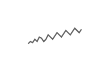
\begin{tikzpicture}[x=0.08em, y=0.08em, line width=0.4pt]
                \draw[FooterGray] (0,3) -- (1,4) -- (2,3.5) -- (3,5) -- (4,4) -- (5,6) -- (6,5.5) -- (7,4) -- (8,5) -- (9,7) -- (10,6) -- (11,5) -- (12,6.5) -- (13,8) -- (14,7) -- (15,6) -- (16,7.5) -- (17,9) -- (18,8) -- (19,7) -- (20,8.5) -- (21,10) -- (22,9) -- (23,8) -- (24,9.5);
            \end{tikzpicture}%
        }%
        \hskip0.5cm%
    }%
    \vskip6pt%
}

%=============================================================================
% PACHETE
%=============================================================================
\usepackage[utf8]{inputenc}
\usepackage[T1]{fontenc}
\usepackage{amsmath, amssymb, amsthm}
\usepackage{mathtools}
\usepackage{bm}
\usepackage{tikz}
\usetikzlibrary{arrows.meta, positioning, shapes, calc, decorations.pathreplacing, shadings}
\usepackage{booktabs}
\usepackage{multirow}
\usepackage{array}
\usepackage{graphicx}
\usepackage{hyperref}
\usepackage{colortbl}
\hypersetup{colorlinks=true, linkcolor=MainBlue, urlcolor=MainBlue}
\graphicspath{{../../logos/}{../../charts/}{../../photos/}}
\hfuzz=2pt  % Suppress tiny overfull warnings (<2pt)
\vfuzz=2pt  % Suppress tiny vertical overfull warnings (<2pt)

%=============================================================================
% COMANDA QUANTLET
%=============================================================================
\newcommand{\quantlet}[2]{%
    \hfill\href{#2}{%
        \raisebox{-0.15em}{
\includegraphics[height=0.7em]{ql_logo.png}}%
        \textcolor{MainBlue}{\tiny\ #1}%
    }%
}

%=============================================================================
% PAGINĂ TITLU PERSONALIZATĂ
%=============================================================================
\defbeamertemplate*{title page}{hybrid}[1][]
{
    \vspace{0.2cm}
    % Rând logo-uri - antet superior (cu linkuri clickabile)
    \begin{center}
        \href{https://www.ase.ro}{
\includegraphics[height=1.0cm]{ase_logo.png}}\hspace{0.3cm}%
        \href{https://theida.net}{
\includegraphics[height=1.0cm]{ida_logo.png}}\hspace{0.3cm}%
        \href{https://blockchain-research-center.com}{
\includegraphics[height=1.0cm]{brc_logo.png}}\hspace{0.3cm}%
        \href{https://www.ai4efin.ase.ro}{
\includegraphics[height=1.0cm]{ai4efin_logo.png}}\hspace{0.3cm}%
        \href{https://ipe.ro/new}{
\includegraphics[height=1.0cm]{acad_logo.png}}\hspace{0.3cm}%
        \href{https://www.digital-finance-msca.com}{
\includegraphics[height=1.0cm]{msca_logo.png}}%
    \end{center}

    \vspace{0.6cm}

    % Titlu principal cu logo-uri Q pe părți (cu linkuri clickabile)
    \begin{center}
        \begin{minipage}{0.1\textwidth}
            \centering
            \href{https://quantlet.com}{
\includegraphics[height=1.1cm]{ql_logo.png}}
        \end{minipage}%
        \begin{minipage}{0.78\textwidth}
            \centering
            {\LARGE\bfseries\usebeamercolor[fg]{title}\inserttitle}

            \vspace{0.3cm}

            {\usebeamerfont{subtitle}\usebeamercolor[fg]{title}\insertsubtitle}
        \end{minipage}%
        \begin{minipage}{0.1\textwidth}
            \centering
            \href{https://quantinar.com}{
\includegraphics[height=1.1cm]{qr_logo.png}}
        \end{minipage}
    \end{center}

    \vspace{0.6cm}

    % Autori (aliniere la stânga)
    \hspace{0.5cm}{\usebeamerfont{author}\insertauthor}

    \vspace{0.3cm}

    % Institut/Afilieri (aliniere la stânga)
    \hspace{0.5cm}\begin{minipage}[t]{0.9\textwidth}
        \raggedright\small\insertinstitute
    \end{minipage}
}

%=============================================================================
% MEDII PENTRU TEOREME
%=============================================================================
\theoremstyle{definition}
\setbeamertemplate{theorems}[numbered]
\newtheorem{defn}{Definiție}
\newtheorem{thm}{Teoremă}
\newtheorem{prop}{Propoziție}
\newtheorem{rmk}{Observație}

%=============================================================================
% CENTRED MINIPAGE
%=============================================================================
\newenvironment{cminipage}[1]{%
    \par\noindent\hfill\begin{minipage}{#1}\ignorespaces
}{%
    \end{minipage}\hfill\null\par
}

%=============================================================================
% COMENZI PERSONALIZATE
%=============================================================================
\newcommand{\E}{\mathbb{E}}
\newcommand{\Var}{\text{Var}}
\newcommand{\Cov}{\text{Cov}}
\newcommand{\Corr}{\text{Corr}}
\newcommand{\R}{\mathbb{R}}
\newcommand{\N}{\mathbb{N}}
\newcommand{\Z}{\mathbb{Z}}
\newcommand{\B}{\mathbf{B}}
\newcommand{\imark}{\textcolor{MainBlue}{\textbullet}}
\newcommand{\RMSE}{\text{RMSE}}
\newcommand{\MAE}{\text{MAE}}
\newcommand{\MAPE}{\text{MAPE}}

%=============================================================================
% INFORMAȚII TITLU
%=============================================================================
\title[Statistica Piețelor Financiare]{Statistica Piețelor Financiare}
\subtitle{Capitolul 1: Date și indicatori statistici}
\author[D.T. Pele, A. Amza]{Daniel Traian PELE \\ Antoaneta Amza}
\institute{Academia de Studii Economice din București\\
IDA Institute Digital Assets\\
Blockchain Research Center\\
AI4EFin Artificial Intelligence for Energy Finance\\
Academia Română, Institutul de Prognoză Economică\\
MSCA Digital Finance}
\date{}

\begin{document}

% Pagina de titlu (fără antet/subsol)
{
\setbeamertemplate{headline}{}
\setbeamertemplate{footline}{}
\begin{frame}
    \titlepage
\end{frame}
}

%=============================================================================
% OBIECTIVE DE ÎNVĂȚARE
%=============================================================================
\begin{frame}{Obiective de învățare}
    \begin{block}{La sfârșitul acestui capitol, veți fi capabili să:}
    \begin{enumerate}
        \item[\textcolor{MainBlue}{\textbf{1.}}] \textbf{Distingeți} între date de preț OHLC, prețuri ajustate și spread-uri bid-ask
        \item[\textcolor{MainBlue}{\textbf{2.}}] \textbf{Calculați} randamente simple și logaritmice și explicați pierderea din varianță
        \item[\textcolor{MainBlue}{\textbf{3.}}] \textbf{Identificați} faptele stilizate ale randamentelor (cozi groase, gruparea volatilității, efect levier)
        \item[\textcolor{MainBlue}{\textbf{4.}}] \textbf{Aplicați} estimatori de volatilitate bazați pe range (Parkinson, GK, RS, Yang-Zhang)
        \item[\textcolor{MainBlue}{\textbf{5.}}] \textbf{Comparați} eficiența estimatorilor și volatilitatea condițională vs.\ necondițională
        \item[\textcolor{MainBlue}{\textbf{6.}}] \textbf{Calculați} măsuri de performanță ajustate la risc (Sharpe, Sortino, Calmar)
        \item[\textcolor{MainBlue}{\textbf{7.}}] \textbf{Construiți} frontiera eficientă și derivați portofoliul cu varianță minimă
    \end{enumerate}
    \end{block}
\end{frame}

%=============================================================================
% CUPRINS
%=============================================================================
{
\setbeamertemplate{headline}{%
    \vskip10pt%
    \hbox to \paperwidth{\hskip0.5cm\hfill\hskip0.5cm}%
    \vskip4pt%
    {\color{FooterGray}\hrule height 0.4pt}%
}
\begin{frame}{}
    {\color{FooterGray}\hrule height 0.4pt}
    \vspace{0.1cm}
    {\Large\textcolor{IDAred}{\textbf{Cuprins}}}
    \vspace{0.2cm}
    {\small
    \begin{columns}[T]
        \begin{column}{0.48\textwidth}
            \begin{enumerate}
                \item Motivație
                \item Date de preț
                \item Randamente
                \item Fapte stilizate
                \item Estimatori de volatilitate
                \item Comparație de eficiență
            \end{enumerate}
        \end{column}
        \begin{column}{0.48\textwidth}
            \begin{enumerate}\setcounter{enumi}{6}
                \item Randamente ajustate la risc
                \item Caz de utilizare AI
                \item Rezumat
                \item Quiz
                \item Bibliografie
            \end{enumerate}
        \end{column}
    \end{columns}
    }
\end{frame}
}

%=============================================================================
% HARTA CAPITOLULUI
%=============================================================================
\begin{frame}{Harta capitolului}
\begin{center}

\begin{tikzpicture}[>=Stealth, node distance=0.7cm, every node/.style={font=\small}]
    % Main flow
    \node[draw, rounded corners, fill=MainBlue!15, minimum width=1.9cm, minimum height=1.0cm, text width=1.7cm, align=center] (data) {\textbf{Date}\\ \footnotesize OHLC, volum};
    \node[draw, rounded corners, fill=MainBlue!12, minimum width=1.9cm, minimum height=1.0cm, text width=1.7cm, align=center, right=0.7cm of data] (transf) {\textbf{Transformare}\\ \footnotesize $r_t = \ln(P_t/P_{t-1})$};
    \node[draw, rounded corners, fill=MainBlue!10, minimum width=1.9cm, minimum height=1.0cm, text width=1.7cm, align=center, right=0.7cm of transf] (prop) {\textbf{Proprietăți}\\ \footnotesize asimetrie, kurtosis};
    \node[draw, rounded corners, fill=Amber!25, minimum width=1.9cm, minimum height=1.0cm, text width=1.7cm, align=center, right=0.7cm of prop] (risk) {\textbf{Estimare risc}\\ \footnotesize $\sigma_t$, MDD};
    \node[draw, rounded corners, fill=Forest!15, minimum width=1.9cm, minimum height=1.0cm, text width=1.7cm, align=center, right=0.7cm of risk] (dec) {\textbf{Decizie}\\ \footnotesize Sharpe, portofoliu};
    \draw[->, thick, MainBlue] (data) -- (transf);
    \draw[->, thick, MainBlue] (transf) -- (prop);
    \draw[->, thick, Amber] (prop) -- (risk);
    \draw[->, thick, Forest] (risk) -- (dec);
\end{tikzpicture}
\end{center}
\vspace{0.3cm}
\begin{columns}[T]
\begin{column}{0.48\textwidth}
\begin{block}{Parcursul logic}
\begin{itemize}
    \item Colectăm \textbf{date de preț} (OHLC)
    \item Le transformăm în \textbf{randamente}
    \item Studiem \textbf{faptele stilizate}
    \item Estimăm \textbf{riscul} (volatilitate, drawdown)
    \item Luăm \textbf{decizii} (Sharpe, frontieră eficientă)
\end{itemize}
\end{block}
\end{column}
\begin{column}{0.48\textwidth}
\begin{exampleblock}{Ideea centrală}
\begin{itemize}
    \item Prețurile sunt \textbf{nestaționare} --- nu le putem modela direct
    \item Randamentele sunt \textbf{staționare} --- le putem analiza statistic
    \item Volatilitatea este o \textbf{variabilă latentă} --- trebuie estimată
    \item Riscul nu este doar volatilitate --- include cozi groase, drawdown, asimetrie
\end{itemize}
\end{exampleblock}
\end{column}
\end{columns}
\end{frame}

%=============================================================================
% TITLU PARTEA I
%=============================================================================
{
\setbeamertemplate{headline}{}
\setbeamertemplate{footline}{}
\begin{frame}[plain]
\vfill
\begin{center}
{\Huge\textcolor{IDAred}{\textbf{Partea I}}}

\vspace{0.6cm}

{\Large\textcolor{MainBlue}{Date, Randamente și Fapte Stilizate}}

\vspace{0.4cm}

{\large\textcolor{MediumGray}{--- Secțiunile 1--4 ---}}
\end{center}
\vfill
\end{frame}
}

%=============================================================================
% SECȚIUNEA 1: MOTIVAȚIE
%=============================================================================
\section{Motivație}

\begin{frame}[shrink=8]{De ce avem nevoie de date?}
\begin{columns}[T]
\begin{column}{0.30\textwidth}
\begin{center}

\includegraphics[width=\linewidth]{data_data.jpeg}
\end{center}
\vspace{-0.2cm}
{\tiny\textit{``Data! Data! Data! I can't make bricks without clay.''} --- Sherlock Holmes}
\end{column}
\begin{column}{0.33\textwidth}
\begin{block}{Înțelegerea trecutului}
\begin{itemize}
    \item Identificarea modelelor, tendințelor și anomaliilor.
    \item Validarea teoriilor: EMH (\textit{Efficient Market Hypothesis}), CAPM (\textit{Capital Asset Pricing Model}), APT (\textit{Arbitrage Pricing Theory}).
    \item Măsurarea profilurilor de risc și randament.
\end{itemize}
\end{block}
\vspace{0.05cm}
\begin{block}{Predicția viitorului}
\begin{itemize}
    \item Prognoza prețurilor, volatilității, corelațiilor.
    \item Construirea de strategii cantitative.
    \item Analiză de scenarii și stress testing.
\end{itemize}
\end{block}
\end{column}
\begin{column}{0.33\textwidth}
\begin{block}{Managementul riscului}
\begin{itemize}
    \item Cuantificarea expunerii: VaR (\textit{Value at Risk}), CVaR (\textit{Conditional VaR}), ES (\textit{Expected Shortfall}).
    \item Diversificarea portofoliului și hedging.
    \item Conformitate regulatorie (Basel III, Solvency II).
\end{itemize}
\end{block}
\vspace{0.05cm}
\begin{block}{Evaluare \& tranzacționare}
\begin{itemize}
    \item Evaluarea derivatelor (opțiuni, futures, swap-uri).
    \item Contabilizare mark-to-market.
    \item Tranzacționare algoritmică și de înaltă frecvență.
\end{itemize}
\end{block}
\end{column}
\end{columns}
\end{frame}

\begin{frame}{Exemple de utilizare a datelor}
\begin{columns}[T]
\begin{column}{0.48\textwidth}
\begin{block}{Analiză tehnică}
\begin{itemize}
    \item Utilizează date istorice de preț și volum.
    \item Modele grafice, medii mobile, RSI, MACD.
    \item Presupune că istoria prețurilor se repetă.
\end{itemize}
\end{block}
\vspace{0.15cm}
\begin{block}{Analiză fundamentală}
\begin{itemize}
    \item Situații financiare, câștiguri, indicatori macro.
    \item Modele de fluxuri de numerar actualizate (DCF).
    \item Raportul P/E, book-to-market, randamentul dividendelor.
\end{itemize}
\end{block}
\end{column}
\begin{column}{0.48\textwidth}
\begin{block}{Finanțe cantitative}
\begin{itemize}
    \item Modele statistice: GARCH, vol. stochastică, copule.
    \item Învățare automată: random forests, LSTM-uri.
    \item Modele factoriale: Fama-French, Carhart, Barra.
\end{itemize}
\end{block}
\vspace{0.15cm}
\begin{block}{Tranzacționare algoritmică}
\begin{itemize}
    \item Date tick-by-tick, registrul de ordine (\textit{order book}), date TAQ.
    \item Algoritmi de execuție sensibili la latență.
    \item Microstructura pieței și execuția optimă.
\end{itemize}
\end{block}
\end{column}
\end{columns}
\end{frame}

\begin{frame}{Surse de date}
\begin{center}
{\scriptsize
\renewcommand{\arraystretch}{1.3}
\begin{tabular}{llll}
\toprule
\textbf{Sursă} & \textbf{Tip} & \textbf{Cost} & \textbf{Acoperire} \\
\midrule
Bloomberg Terminal & OHLCV, fundamentale, știri & \$\$\$\$ & Global, toate clasele de active \\
Refinitiv Eikon & OHLCV, date tick, știri & \$\$\$ & Global, instituțional \\
Yahoo Finance & OHLCV zilnic, dividende & Gratuit & Acțiuni, ETF-uri, FX \\
WRDS / CRSP & Prețuri ajustate, randamente & \$\$ (academic) & Acțiuni SUA, 1926--prezent \\
CoinGecko / CoinMarketCap & OHLCV, date on-chain & Gratuit/\$ & Criptomonede \\
\bottomrule
\end{tabular}
}
\end{center}
\vspace{0.15cm}
\begin{columns}[T]
\begin{column}{0.48\textwidth}
\begin{block}{Surse gratuite}
\begin{itemize}
    \item Yahoo Finance, Alpha Vantage, Quandl (NASDAQ Data Link).
    \item Suficiente pentru cercetare academică și backtesting.
    \item Întârzieri: 15--20 minute pentru cotații în timp real.
\end{itemize}
\end{block}
\end{column}
\begin{column}{0.48\textwidth}
\begin{block}{Surse plătite / instituționale}
\begin{itemize}
    \item Bloomberg, Refinitiv: date tick la nivel de milisecundă.
    \item WRDS/CRSP: date curate de acțiuni SUA, fără survivorship bias.
    \item Esențiale pentru managementul profesional al riscului.
\end{itemize}
\end{block}
\end{column}
\end{columns}
\end{frame}

\begin{frame}{Frecvența datelor}
\begin{center}
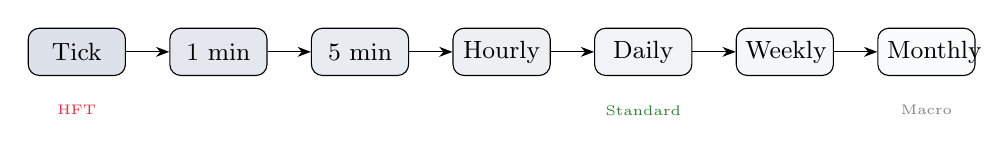
\begin{tikzpicture}[>=Stealth, node distance=0.9cm, every node/.style={font=\small}]
    \node[draw, rounded corners, fill=MainBlue!15, minimum width=1.1cm, minimum height=0.6cm, text width=1.0cm, align=center] (tick) {Tick};
    \node[draw, rounded corners, fill=MainBlue!12, minimum width=1.1cm, minimum height=0.6cm, text width=1.0cm, align=center, right=0.55cm of tick] (m1) {1 min};
    \node[draw, rounded corners, fill=MainBlue!10, minimum width=1.1cm, minimum height=0.6cm, text width=1.0cm, align=center, right=0.55cm of m1] (m5) {5 min};
    \node[draw, rounded corners, fill=MainBlue!8, minimum width=1.1cm, minimum height=0.6cm, text width=1.0cm, align=center, right=0.55cm of m5] (hr) {Hourly};
    \node[draw, rounded corners, fill=MainBlue!6, minimum width=1.1cm, minimum height=0.6cm, text width=1.0cm, align=center, right=0.55cm of hr] (day) {Daily};
    \node[draw, rounded corners, fill=MainBlue!4, minimum width=1.1cm, minimum height=0.6cm, text width=1.0cm, align=center, right=0.55cm of day] (wk) {Weekly};
    \node[draw, rounded corners, fill=MainBlue!2, minimum width=1.1cm, minimum height=0.6cm, text width=1.0cm, align=center, right=0.55cm of wk] (mo) {Monthly};
    \draw[->] (tick) -- (m1);
    \draw[->] (m1) -- (m5);
    \draw[->] (m5) -- (hr);
    \draw[->] (hr) -- (day);
    \draw[->] (day) -- (wk);
    \draw[->] (wk) -- (mo);
    \node[below=0.25cm of tick, font=\tiny, text=Crimson] {HFT};
    \node[below=0.25cm of day, font=\tiny, text=Forest] {Standard};
    \node[below=0.25cm of mo, font=\tiny, text=MediumGray] {Macro};
\end{tikzpicture}
\end{center}
\vspace{0.1cm}
\begin{itemize}
    \item \textbf{Frecvență mai mare} $\Rightarrow$ mai multe observații, mai mult zgomot de microstructură.
    \item \textbf{Zilnic} este frecvența standard pentru cercetarea academică și practică.
    \item \textbf{Efectul Epps} (1979): corelațiile perechi între active \textit{scad} pe măsură ce frecvența de eșantionare crește către nivelul de tick.
    \begin{itemize}
        \item Cauzat de tranzacționarea asincronă: activele nu se tranzacționează simultan.
        \item Corelațiile măsurate la frecvență zilnică sunt semnificativ mai mari decât la 1 minut.
    \end{itemize}
    \item \textbf{Datele intrazilnice} sunt esențiale pentru estimarea volatilității realizate (Secțiunea 5).
\end{itemize}
\end{frame}

\begin{frame}{Provocări ale datelor în finanțe}
\begin{itemize}
    \item \textbf{Calitatea datelor}: Valori lipsă, tick-uri eronate, erori la acțiuni corporative.
    \begin{itemize}
        \item Chiar și datele Bloomberg conțin erori; validați mereu.
    \end{itemize}
    \item \textbf{Survivorship bias}: Studierea doar a firmelor listate curent inflează randamentele estimate.
    \begin{itemize}
        \item CRSP include firmele delistate; Yahoo Finance nu.
    \end{itemize}
    \item \textbf{Look-ahead bias}: Utilizarea informațiilor indisponibile la momentul deciziei.
    \begin{itemize}
        \item Ex., utilizarea compoziției actuale a indicelui pentru a backtesta o strategie de 10 ani.
    \end{itemize}
    \item \textbf{Volumul datelor}: HFT generează $\sim$1 TB/zi per bursă; stocarea și curățarea sunt netriviale.
    \item \textbf{Testare multiplă}: Harvey, Liu \& Zhu (2016) argumentează că majoritatea factorilor publicați sunt descoperiri false.
    \begin{itemize}
        \item $p$-hacking și căutarea excesivă în date inflează erorile de tip I.
        \item Prag recomandat: $t$-statistic $> 3.0$ pentru factori noi.
    \end{itemize}
    \item \textbf{Interpretarea datelor}: Corelație $\neq$ cauzalitate; semnificație statistică $\neq$ economică.
\end{itemize}
\end{frame}

%=============================================================================
% ACTUALIZARE CUPRINS după Secțiunea 1
%=============================================================================
{
\setbeamertemplate{headline}{%
    \vskip10pt%
    \hbox to \paperwidth{\hskip0.5cm\hfill\hskip0.5cm}%
    \vskip4pt%
    {\color{FooterGray}\hrule height 0.4pt}%
}
\begin{frame}{}
    {\color{FooterGray}\hrule height 0.4pt}
    \vspace{0.1cm}
    {\Large\textcolor{IDAred}{\textbf{Cuprins}}}
    \vspace{0.2cm}
    \begin{enumerate}
        \item Motivație \checkmark
        \item \textbf{Date de preț}
        \item Randamente
        \item Fapte stilizate ale randamentelor financiare
        \item Estimatori de volatilitate
        \item Comparație de eficiență
        \item Randamente ajustate la risc
        \item Caz AI / Rezumat / Quiz
        \item Bibliografie
    \end{enumerate}
\end{frame}
}

%=============================================================================
% SECȚIUNEA 2: DATE DE PREȚ
%=============================================================================
\section{Date de preț}

\begin{frame}{Date OHLC}
\begin{columns}[T]
\begin{column}{0.48\textwidth}
\begin{center}
{\small
\renewcommand{\arraystretch}{1.35}
\begin{tabular}{>{\bfseries}lll}
\toprule
Symbol & Denumire & Descriere \\
\midrule
$O_t$ & Deschidere & Primul preț din perioada $t$ \\
$H_t$ & Maxim & Prețul maxim din perioada $t$ \\
$L_t$ & Minim & Prețul minim din perioada $t$ \\
$C_t$ & Închidere & Ultimul preț din perioada $t$ \\
$V_t$ & Volum & Acțiuni tranzacționate \\
\bottomrule
\end{tabular}
}
\end{center}
\vspace{0.15cm}
\begin{itemize}
    \item Prin construcție: $L_t \leq O_t,\, C_t \leq H_t$.
    \item Range $H_t - L_t$: proxy pentru volatilitatea intra-perioadă.
    \item Volum mare $\Rightarrow$ descoperire a prețului mai eficientă.
\end{itemize}
\end{column}
\begin{column}{0.48\textwidth}
\begin{center}
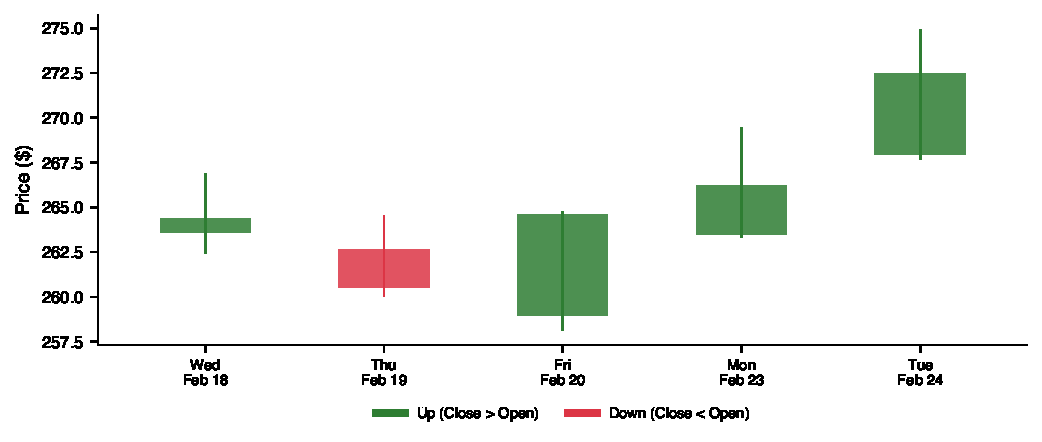
\includegraphics[width=0.85\linewidth]{sfm_ch1_candlestick.pdf}
\end{center}
\end{column}
\end{columns}
\quantlet{SFM\_ch1\_ohlc\_ob}{https://github.com/QuantLet/Stat_fin_markets/tree/master/Ch_01/SFM_ch1_ohlc_orderbook}
\end{frame}

\begin{frame}{OHLC: Exemplu numeric}
\begin{itemize}
    \item Cinci zile de tranzacționare cu date simulate tip AAPL (prețuri în USD):
\end{itemize}
\vspace{0.1cm}
\begin{center}
{\scriptsize
\renewcommand{\arraystretch}{1.3}
\begin{tabular}{lccccc}
\toprule
\textbf{Date} & \textbf{Open} & \textbf{High} & \textbf{Low} & \textbf{Close} & \textbf{Volume} \\
\midrule
2024-01-02 & 185.20 & 188.45 & 184.10 & 187.90 & 52{,}300{,}000 \\
2024-01-03 & 187.90 & 189.30 & 183.60 & 184.20 & 61{,}800{,}000 \\
2024-01-04 & 184.20 & 186.80 & 181.50 & 186.10 & 48{,}500{,}000 \\
2024-01-05 & 186.10 & 191.20 & 185.70 & 190.40 & 55{,}200{,}000 \\
2024-01-08 & 190.40 & 193.50 & 188.90 & 192.30 & 47{,}900{,}000 \\
\bottomrule
\end{tabular}
}
\end{center}
\vspace{0.15cm}
\begin{itemize}
    \item Ziua 2 (3 Ian): \textcolor{Crimson}{lumânare bearish} --- Close $<$ Open; spread $=189.30-183.60=\$5.70$.
    \item Ziua 4 (5 Ian): \textcolor{Forest}{lumânare bullish puternică} --- Close $-$ Open $= \$4.30$; volum mare.
    \item Randamentul logaritmic zilnic, 2 Ian: $r = \ln(187.90/185.20) = 0.01449 \approx 1.45\%$.
\end{itemize}
\quantlet{SFM\_ch1\_ohlc\_ob}{https://github.com/QuantLet/Stat_fin_markets/tree/master/Ch_01/SFM_ch1_ohlc_orderbook}
\end{frame}

\begin{frame}{Prețul ajustat de închidere}
\begin{itemize}
    \item Prețurile de închidere brute \textbf{nu sunt direct comparabile} în timp din cauza acțiunilor corporative.
    \item \textbf{Prețul ajustat de închidere} ține cont retroactiv de toate acțiunile corporative:
\end{itemize}
\[
P_t^{\text{adj}} = P_t \times \prod_{k:\, t_k > t} A_{t_k}^{-1}
\]
\begin{itemize}
    \item $A_{t_k}$ $\succ$ factorul de ajustare la data acțiunii corporative $t_k$
\end{itemize}
\vspace{0.05cm}
\begin{center}
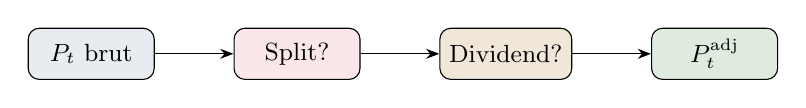
\begin{tikzpicture}[>=Stealth, node distance=1.5cm, every node/.style={font=\small}]
    \node[draw, rounded corners, fill=MainBlue!10, minimum width=1.6cm, minimum height=0.65cm] (raw) {$P_t$ brut};
    \node[draw, rounded corners, fill=Crimson!12, minimum width=1.6cm, minimum height=0.65cm, right=1.0cm of raw] (split) {Split?};
    \node[draw, rounded corners, fill=Amber!20, minimum width=1.6cm, minimum height=0.65cm, right=1.0cm of split] (div) {Dividend?};
    \node[draw, rounded corners, fill=Forest!15, minimum width=1.6cm, minimum height=0.65cm, right=1.0cm of div] (adj) {$P_t^{\text{adj}}$};
    \draw[->] (raw) -- (split);
    \draw[->] (split) -- (div);
    \draw[->] (div) -- (adj);
\end{tikzpicture}
\end{center}
\vspace{0.1cm}
\begin{alertblock}{Important}
\begin{itemize}\setlength{\itemsep}{0pt}
    \item Folosiți mereu prețuri ajustate la calculul randamentelor --- prețurile brute prezintă salturi false la datele acțiunilor corporative care ar apărea ca randamente artificiale mari.
\end{itemize}
\end{alertblock}
\end{frame}

\begin{frame}{Factori individuali de ajustare}
\begin{itemize}
    \item \textbf{Splituri de acțiuni} ($m$-for-$n$): fiecare acționar primește $m$ acțiuni pentru fiecare $n$ deținute.
    \[
    A_t^{\text{split}} = \frac{n}{m}, \qquad \text{de ex.\ split 2-la-1:}\; A_t = \tfrac{1}{2}.
    \]
    \item \textbf{Dividende în acțiuni}: compania emite acțiuni noi ca dividend (de ex.\ 10\% dividend în acțiuni).
    \[
    A_t^{\text{stock div}} = \frac{1}{1+d}, \qquad d = \text{rata dividendului}.
    \]
    \item \textbf{Dividende în numerar}: plată directă în numerar $D_t$ pe acțiune.
    \[
    A_t^{\text{cash div}} = \frac{P_{t-1} - D_t}{P_{t-1}} = 1 - \frac{D_t}{P_{t-1}}.
    \]
    \item \textbf{Oferte de drepturi}: acționarii existenți cumpără acțiuni noi la un preț redus.
    \[
    A_t^{\text{rights}} = \frac{P_{t-1} + r \cdot P_{\text{sub}}}{P_{t-1}(1+r)},
    \]
    unde $r$ = raportul de acțiuni noi per acțiune existentă, $P_{\text{sub}}$ = prețul de subscriere.
\end{itemize}
\end{frame}

\begin{frame}{Exemplu numeric: Prețuri ajustate}
\begin{example}
Acțiune la \$100. Ziua 5: dividend în numerar \$2. Ziua 10: split 2-la-1.
\end{example}
\begin{itemize}
    \item \textbf{Factori de ajustare:} $A_5 = 98/100 = 0.98$;\quad $A_{10} = 1/2 = 0.50$
    \item \textbf{Prețuri ajustate:}
\end{itemize}
\vspace{-0.1cm}
\begin{center}
{\small
\renewcommand{\arraystretch}{1.2}
\begin{tabular}{lll}
\toprule
\textbf{Perioada} & \textbf{Ajustări} & \textbf{Formulă} \\
\midrule
$t < 5$ & ambele & $P_t^{\text{adj}} = P_t \times 0.49$ \\
$5 \leq t < 10$ & doar split & $P_t^{\text{adj}} = P_t \times 0.50$ \\
$t \geq 10$ & niciuna & $P_t^{\text{adj}} = P_t$ \\
\bottomrule
\end{tabular}
}
\end{center}
\vspace{0.05cm}
\begin{itemize}
    \item \$100 din Ziua 1 se ajustează la $100 \times 0.49 = \$49$ retroactiv --- nu e o pierdere, ci doar o ajustare contabilă.
    \item Seria de randamente calculată din prețuri ajustate este continuă pe parcursul acțiunilor corporative.
\end{itemize}
\end{frame}

\begin{frame}{Spread Bid-Ask și registrul de ordine (\textit{order book})}
\begin{itemize}
    \item \textbf{Ask} $P^a$: cel mai mic preț de vânzare.
    \item \textbf{Bid} $P^b$: cel mai mare preț de cumpărare.
    \item \textbf{Spread}: $s = P^a - P^b > 0$.
    \item \textbf{Mid-price}: $P^m = (P^a + P^b)/2$.
    \item \textbf{Effective spread}: $2|P_{\text{trade}} - P^m|$.
    \item Spread-uri mai mici $\Rightarrow$ piață mai lichidă.
\end{itemize}
\vspace{-0.15cm}
\begin{center}
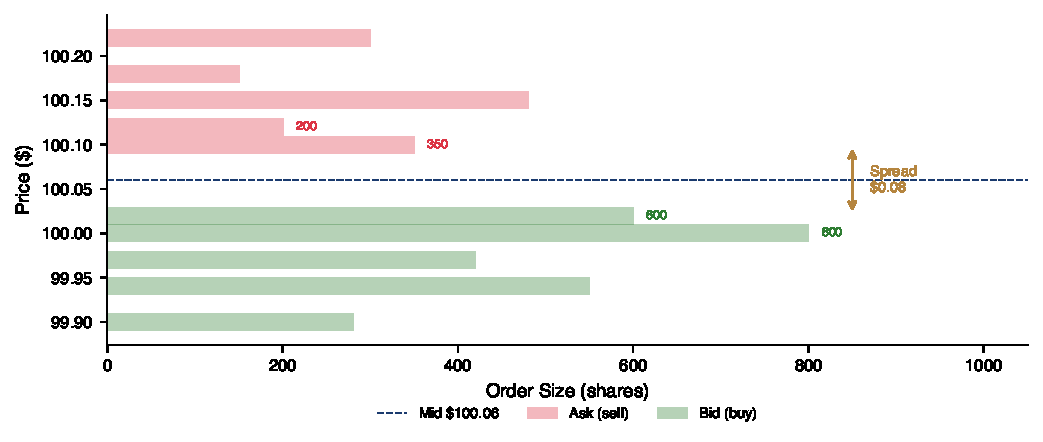
\includegraphics[width=0.55\linewidth]{sfm_ch1_orderbook.pdf}
\end{center}
\quantlet{SFM\_ch1\_ohlc\_ob}{https://github.com/QuantLet/Stat_fin_markets/tree/master/Ch_01/SFM_ch1_ohlc_orderbook}
\end{frame}

\begin{frame}{Microstructura pieței}
\begin{itemize}
    \item \textbf{Microstructura pieței} studiază modul în care se formează prețurile la nivel de tranzacție.
    \item \textbf{Descoperirea prețului}: procesul prin care informațiile noi sunt încorporate în prețuri.
    \begin{itemize}
        \item Roll (1984): saltul bid-ask induce autocorrelație \textit{negativă} de ordinul întâi în randamentele tranzacțiilor.
        \item Prețul tranzacției observat $= $ prețul real $+$ componentă de zgomot.
    \end{itemize}
    \item \textbf{Asimetria informațională}: unii traderi au informații private (traderi informați).
    \begin{itemize}
        \item Formatorii de piață (\textit{market makers}) lărgesc spread-urile când riscul de selecție adversă este mare.
        \item Glosten-Milgrom (1985) model: spread-ul de echilibru depinde de fracția de traderi informați.
    \end{itemize}
    \item \textbf{Market makers}: furnizează lichiditate cotând simultan bid și ask.
    \begin{itemize}
        \item Profită din spread; suportă risc de inventar și selecție adversă.
    \end{itemize}
    \item \textbf{Tick size}: incrementul minim de preț (de ex., \$0,01 pentru acțiunile SUA de la decimalizarea din 2001).
    \begin{itemize}
        \item Tick mai mic $\Rightarrow$ spread-uri mai mici dar potențial mai puțină adâncime.
    \end{itemize}
\end{itemize}
\end{frame}

\begin{frame}{Estimarea spreadului efectiv: Exemplu}
\begin{center}
{\small
\renewcommand{\arraystretch}{1.2}
\begin{tabular}{ccccc}
\toprule
\textbf{Tranzacția} & \textbf{Preț} (\$) & \textbf{Midpoint} (\$) & \textbf{Direcție} & \textbf{Spread efectiv} \\
\midrule
1 & 50.10 & 50.05 & Cumpărare & $2 \times |50.10 - 50.05| = 0.10$ \\
2 & 49.95 & 50.00 & Vânzare & $2 \times |49.95 - 50.00| = 0.10$ \\
3 & 50.15 & 50.08 & Cumpărare & $2 \times |50.15 - 50.08| = 0.14$ \\
4 & 49.90 & 49.95 & Vânzare & $2 \times |49.90 - 49.95| = 0.10$ \\
5 & 50.20 & 50.10 & Cumpărare & $2 \times |50.20 - 50.10| = 0.20$ \\
\bottomrule
\end{tabular}
}
\end{center}
\vspace{0.1cm}
\begin{itemize}\small\setlength{\itemsep}{1pt}
    \item \textbf{Spread efectiv mediu}: $\bar{S}_{\text{eff}} = \frac{1}{5}(0.10+0.10+0.14+0.10+0.20) = \$0.128$.
    \item \textbf{Estimatorul Roll} (1984): $\hat{S} = 2\sqrt{-\widehat{\text{Cov}}(\Delta P_t, \Delta P_{t-1})}$ --- estimează spreadul doar din autocovarianța randamentelor, fără date de cotații.
    \item Aplicabil când datele bid/ask nu sunt disponibile (serii istorice lungi).
\end{itemize}
\end{frame}

\begin{frame}{Impactul de piață și conținutul informațional}
\begin{itemize}\setlength{\itemsep}{2pt}
    \item \textbf{Impactul de piață} (\textit{market impact}): deplasarea prețului cauzată de o tranzacție mare.
    \begin{itemize}
        \item Impact temporar (revenire) + impact permanent (informație nouă).
        \item Modelul Almgren-Chriss (2001): cost total $\propto \sigma \sqrt{V/\text{ADV}}$.
    \end{itemize}
    \item \textbf{Lambda Kyle} ($\lambda$): sensibilitatea prețului la fluxul net de ordine (\textit{order flow}):
    \[
    \Delta P_t = \lambda \cdot \text{OF}_t + \varepsilon_t, \qquad \lambda = \text{măsura illichidității informaționale}.
    \]
    \item \textbf{Descompunerea spreadului} (Huang \& Stoll, 1997):
    \begin{itemize}
        \item Componenta de \textit{selecție adversă} (informație) --- compensează pierderea față de traderii informați
        \item Componenta de \textit{inventar} --- risc de deținere a unei poziții dezechilibrate
        \item Componenta de \textit{procesare ordine} --- costuri fixe operaționale
    \end{itemize}
    \item \textbf{Legătura cu MDH}: lichiditatea scăzută $\Rightarrow$ volatilitate mai mare, consistentă cu ipoteza mixturii de distribuții.
\end{itemize}
\end{frame}

%=============================================================================
% ACTUALIZARE CUPRINS după Secțiunea 2
%=============================================================================
{
\setbeamertemplate{headline}{%
    \vskip10pt%
    \hbox to \paperwidth{\hskip0.5cm\hfill\hskip0.5cm}%
    \vskip4pt%
    {\color{FooterGray}\hrule height 0.4pt}%
}
\begin{frame}{}
    {\color{FooterGray}\hrule height 0.4pt}
    \vspace{0.1cm}
    {\Large\textcolor{IDAred}{\textbf{Cuprins}}}
    \vspace{0.2cm}
    \begin{enumerate}
        \item Motivație \checkmark
        \item Date de preț \checkmark
        \item \textbf{Randamente}
        \item Fapte stilizate ale randamentelor financiare
        \item Estimatori de volatilitate
        \item Comparație de eficiență
        \item Randamente ajustate la risc
        \item Caz AI / Rezumat / Quiz
        \item Bibliografie
    \end{enumerate}
\end{frame}
}

%=============================================================================
% SECȚIUNEA 3: RANDAMENTE
%=============================================================================
\section{Randamente}

\begin{frame}{De ce randamente? Staționaritate}
\begin{defn}[Staționaritate slabă (în covarianță)]
\begin{itemize}\setlength{\itemsep}{1pt}
    \item O serie temporală $\{X_t\}$ este \textbf{slab staționară} dacă:
\end{itemize}
\begin{enumerate}
    \item $\E[X_t] = \mu$ \quad (medie constantă, $\forall\, t$),
    \item $\Var(X_t) = \sigma^2 < \infty$ \quad (varianță constantă și finită, $\forall\, t$),
    \item $\Cov(X_t, X_{t-k}) = \gamma(k)$ \quad (autocovarianța depinde doar de lag-ul $k$, nu de $t$).
\end{enumerate}
\end{defn}
\vspace{0.1cm}
\begin{itemize}
    \item \textbf{Prețurile} $P_t$ sunt în general \textbf{nestaționare}: au trend, rădăcini unitare și varianță variabilă în timp.
    \item \textbf{Randamentele} $r_t = \ln(P_t/P_{t-1})$ sunt aproximativ staționare: medie și varianță relativ constante.
    \item \textbf{Notație formală (ordine de integrare)}:
    \[
    P_t \sim I(1) \quad \text{(nestaționară, rădăcină unitară)}, \qquad r_t = \Delta \ln P_t \sim I(0) \quad \text{(staționară)}.
    \]
    \item \textbf{Intuiție}: \textit{„Prețurile cresc, randamentele oscilează."} Analizăm randamente deoarece metodele statistice cer staționaritate.
    \item \textbf{Test formal}: testul Augmented Dickey-Fuller (ADF) respinge ipoteza nulă de rădăcină unitară pentru randamente, dar nu pentru prețuri.
\end{itemize}
\end{frame}

\begin{frame}{Staționaritate: Preț vs.\ Randamente}
\begin{center}
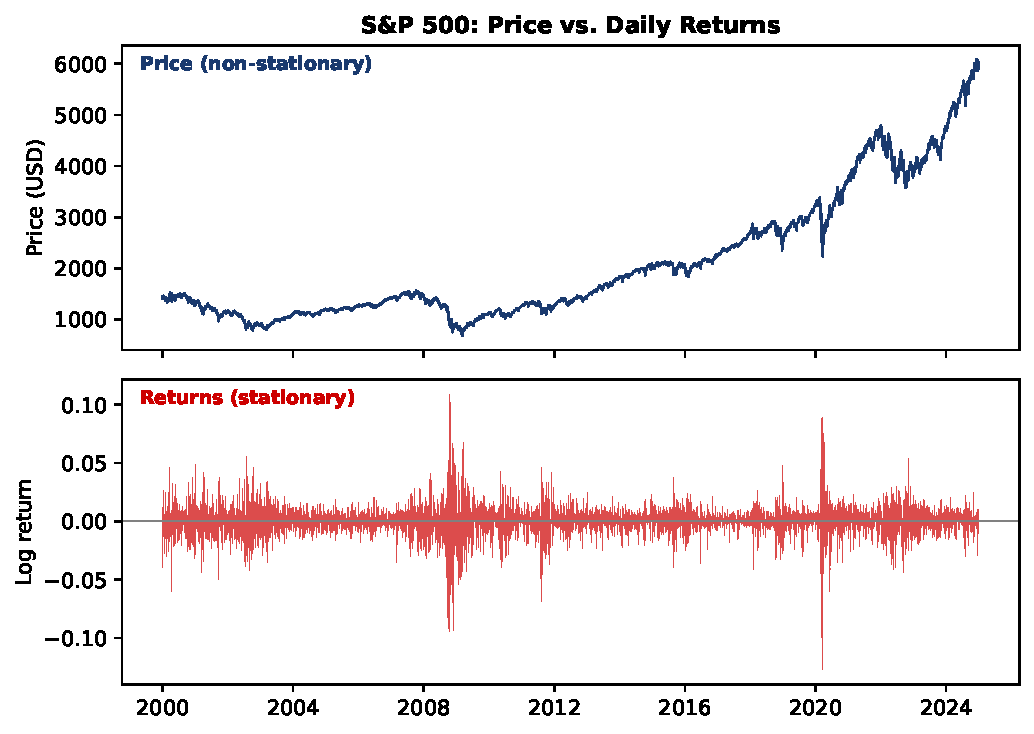
\includegraphics[width=0.85\linewidth]{sfm_ch1_stationarity.pdf}
\end{center}
\vspace{-0.2cm}
\begin{itemize}
    \item \textbf{Sus}: Prețul S\&P 500 are medie cu trend și varianță crescătoare $\Rightarrow$ nestaționară.
    \item \textbf{Jos}: Randamentele log fluctuează în jurul zero-ului cu varianță aprox.\ constantă $\Rightarrow$ staționară.
\end{itemize}
\quantlet{SFM\_ch1\_stationarity}{https://github.com/QuantLet/Stat_fin_markets/tree/master/Ch_01/SFM_ch1_stationarity}
\end{frame}

\begin{frame}{Testul Augmented Dickey-Fuller (ADF)}
\vspace{-0.1cm}
\begin{itemize}\footnotesize\setlength{\itemsep}{0pt}
    \item \textbf{ADF} testează $H_0$: rădăcină unitară (nestaționară) vs.\ $H_1$: staționară.
    \item Model: $\Delta y_t = \alpha + \beta t + \gamma\, y_{t-1} + \sum_{j=1}^{p}\delta_j\,\Delta y_{t-j} + \varepsilon_t$. Respingem $H_0$ dacă $\hat{\tau} = \hat{\gamma}/\text{SE}(\hat{\gamma}) < \tau_{\text{critic}}$.
\end{itemize}
\vspace{-0.2cm}
\begin{center}
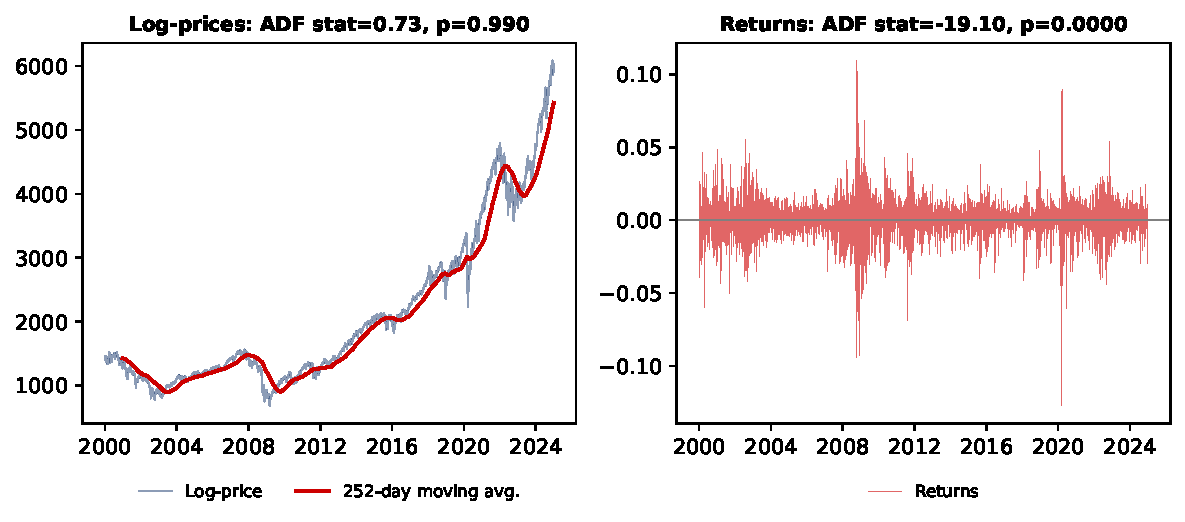
\includegraphics[width=0.72\linewidth]{sfm_ch1_adf_test.pdf}
\end{center}
\vspace{-0.3cm}
\begin{itemize}\small\setlength{\itemsep}{0pt}
    \item Log-prețurile: $H_0$ \textbf{nu} se respinge ($p=0.98$) $\Rightarrow$ rădăcină unitară, $I(1)$.
    \item Log-randamentele: $H_0$ se respinge la 1\% ($p \approx 0$) $\Rightarrow$ staționare, $I(0)$.
\end{itemize}
\quantlet{SFM\_ch1\_stationarity}{https://github.com/QuantLet/Stat_fin_markets/tree/master/Ch_01/SFM_ch1_stationarity}
\end{frame}

\begin{frame}[shrink=8]{Randamente simple (aritmetice)}
\begin{alertblock}{Convenție de notație}
\begin{itemize}\small\setlength{\itemsep}{0pt}
    \item În notația OHLC, prețul de închidere este $C_t$. Însă, de aici înainte, $P_t$ denotă \textbf{prețul de închidere} (\textit{closing price}) sau \textbf{prețul de închidere ajustat} (\textit{adjusted closing price}), în funcție de context.
    \item Folosiți mereu prețuri ajustate pentru calculul randamentelor, pentru a ține cont de dividende și split-uri.
\end{itemize}
\end{alertblock}
\begin{defn}[Randament simplu]
\begin{itemize}\setlength{\itemsep}{1pt}
    \item \textbf{Randamentul net simplu} pe o perioadă:
    $R_t = \frac{P_t - P_{t-1}}{P_{t-1}} = \frac{P_t}{P_{t-1}} - 1.$
    \item \textbf{Randamentul brut}: $1 + R_t = P_t / P_{t-1}$.
\end{itemize}
\end{defn}
\vspace{0.1cm}
\begin{itemize}
    \item \textbf{Aditivitate pe active}: randamentul portofoliului $R_P = \sum_{i=1}^n w_i R_i$ (exact, o perioadă).
    \item \textbf{Nu este aditiv în timp}: randamentul brut multi-perioadă $= \prod_{s}(1+R_s)$, nu o sumă.
    \item \textbf{Mărginit inferior} de $-1$ (răspundere limitată; prețurile nu pot fi negative).
    \item Randamentul brut pe $k$ perioade: $1 + R_t(k) = \prod_{j=0}^{k-1}(1 + R_{t-j})$.
    \item Exemplu: $P_0=100$, $P_1=110$ $\Rightarrow$ $R_1 = 10\%$.
\end{itemize}
\vspace{0.05cm}
\begin{itemize}
    \item \textbf{Observație}: Randamentele simple sunt preferate pentru analiza \textbf{cross-secțională} (construcția portofoliului).
\end{itemize}
\end{frame}

\begin{frame}{Când folosim fiecare tip de randament?}
\begin{center}
{\small
\renewcommand{\arraystretch}{1.4}
\begin{tabular}{>{\bfseries}lll}
\toprule
\textbf{Context} & \textbf{Tip preferat} & \textbf{Motivare} \\
\midrule
Analiză cross-secțională & Simplu ($R_t$) & Aditivitate pe active: $R_P = \sum w_i R_i$ \\
Serie temporală & Logaritmic ($r_t$) & Aditivitate temporală: $r_{0 \to T} = \sum r_t$ \\
Construcție portofoliu & Simplu & Ponderile sunt semnificative \\
Backtesting pe termen lung & Logaritmic & $\ln W_T = \ln W_0 + \sum r_t$ \\
Raportare către investitori & Simplu & Interpretare directă: ``$+10\%$'' \\
Modelare statistică & Logaritmic & $r_t \in (-\infty, +\infty)$, compatibil cu Distribuția Normală \\
\bottomrule
\end{tabular}
}
\end{center}
\vspace{0.2cm}
\begin{exampleblock}{Mini-exercițiu}
\begin{itemize}\setlength{\itemsep}{0pt}
    \item O acțiune are $P_0 = 50$, $P_1 = 55$, $P_2 = 48$. Calculați randamentele simple și logaritmice pentru fiecare perioadă. Verificați: suma log-randamentelor $=$ log-randamentul total?
\end{itemize}
\end{exampleblock}
\end{frame}

\begin{frame}{Randamente logaritmice (compuse continuu)}
\begin{defn}[Randament logaritmic]
\begin{itemize}\setlength{\itemsep}{1pt}
    \item \textbf{Randamentul logaritmic} (randament compus continuu):
    $r_t = \ln\!\left(\frac{P_t}{P_{t-1}}\right) = \ln(1 + R_t).$
\end{itemize}
\end{defn}
\vspace{0.1cm}
\begin{itemize}
    \item \textbf{Aditive în timp}: $r_t(k) = \sum_{j=0}^{k-1} r_{t-j} = \ln(P_t / P_{t-k})$.
    \item \textbf{Non-aditive pe active}: $r_P \neq \sum_i w_i r_i$ în general.
    \item \textbf{Simetrice}: câștig de $+x$ și pierdere de $-x$ tratate simetric.
    \item \textbf{Nemărginite}: $r_t \in (-\infty, +\infty)$, compatibil cu distribuția normală.
    \item Exemplu: $P_0=100$, $P_1=110$ $\Rightarrow$ $r_1 = \ln(1.10) = 9.531\%$.
\end{itemize}
\vspace{0.05cm}
\begin{itemize}
    \item \textbf{Observație}: Randamentele logaritmice sunt preferate pentru analiza \textbf{seriilor de timp} (staționaritate, agregare).
\end{itemize}
\end{frame}

\begin{frame}{Randamente simple vs.\ logaritmice: Expansiunea Taylor}
\begin{prop}
Pentru randamente mici: $r_t = \ln(1+R_t) = R_t - \dfrac{R_t^2}{2} + \dfrac{R_t^3}{3} - \cdots$

La ordinul doi: $r_t \approx R_t - \dfrac{R_t^2}{2}$, deci $r_t < R_t$ pentru orice $R_t \neq 0$.
\end{prop}
\begin{itemize}
    \item \textbf{Demonstrație.}\quad Deoarece $\ln$ este strict concavă, $\ln(1+x) < x$ pentru orice $x > -1$, $x \neq 0$. Substituind $x = R_t$ obținem $r_t = \ln(1+R_t) < R_t$.\hfill$\square$
\end{itemize}
\vspace{0.1cm}
\begin{itemize}
    \item Pentru randamente zilnice ($|R_t|\approx1\%$), aproximarea $r_t \approx R_t$ este excelentă.
    \item Diferența $R_t - r_t \approx R_t^2/2$ crește cu volatilitatea și pe orizonturi mai lungi.
    \item Aceasta este sursa \textbf{pierderii din varianță} în performanța pe termen lung.
\end{itemize}
\begin{alertblock}{Pierderea din varianță (\textit{variance drag}, Inegalitatea lui Jensen)}
\begin{itemize}\setlength{\itemsep}{0pt}
    \item $\E[r_t] = \E[\ln(1+R_t)] < \ln(1+\E[R_t])$. Practic: $\E[r_t] \approx \E[R_t] - \tfrac{1}{2}\Var(R_t)$.
\end{itemize}
\end{alertblock}
\end{frame}

\begin{frame}{Randamente simple vs.\ logaritmice: Comparație vizuală}
\vspace{-0.1cm}
\begin{center}
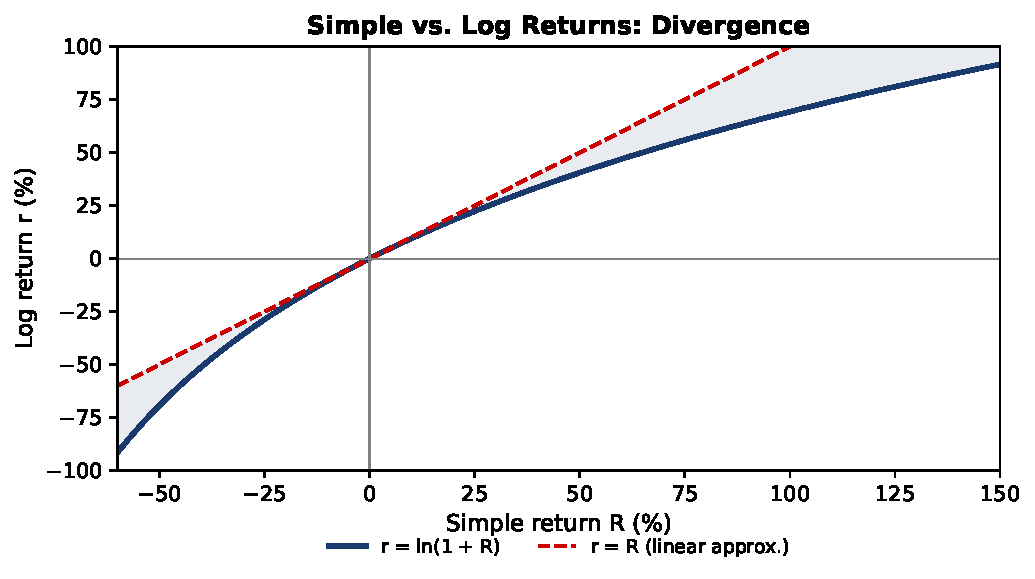
\includegraphics[width=0.75\linewidth]{sfm_ch1_returns_divergence.pdf}
\end{center}
\vspace{-0.3cm}
\begin{itemize}\footnotesize\setlength{\itemsep}{0pt}
    \item Pentru randamente zilnice tipice ($\pm 3\%$), simple $\approx$ log; pentru mișcări mari, divergența e semnificativă.
    \item Randamentul log este mereu \textbf{mai mic} decât cel simplu: $r_t < R_t$ pentru $R_t > 0$.
\end{itemize}
\quantlet{SFM\_ch1\_stationarity}{https://github.com/QuantLet/Stat_fin_markets/tree/master/Ch_01/SFM_ch1_stationarity}
\end{frame}

\begin{frame}{Exemplu numeric: Randamente simple vs.\ logaritmice}
\begin{example}
$P_0 = \$100$: crește $+10\%$ apoi scade $-10\%$ (randamente simple).
\end{example}
\vspace{0.1cm}
\begin{columns}[T]
\begin{column}{0.48\textwidth}
\begin{itemize}
    \item \textbf{Randamente simple:}
    \begin{itemize}
        \item $P_1 = 100 \times 1.10 = \$110$
        \item $P_2 = 110 \times 0.90 = \$99$
        \item Net: $-1\%$. Suma $+10\%-10\%=0$ este \textit{înșelătoare}!
    \end{itemize}
    \item \textbf{Randamente logaritmice:}
    \begin{itemize}
        \item $r_1 = \ln(1.10) = +9.531\%$
        \item $r_2 = \ln(0.90) = -10.536\%$
        \item Sumă: $-1.005\% = \ln(99/100)$ \checkmark
    \end{itemize}
\end{itemize}
\end{column}
\begin{column}{0.48\textwidth}
\begin{center}
{\small
\renewcommand{\arraystretch}{1.3}
\begin{tabular}{lccc}
\toprule
 & Per.\ 1 & Per.\ 2 & \textbf{Total} \\
\midrule
$R_t$ & $+10.00\%$ & $-10.00\%$ & $-1.00\%$ \\
$r_t$ & $+9.53\%$ & $-10.54\%$ & $-1.01\%$ \\
\bottomrule
\end{tabular}
}
\end{center}
\vspace{0.2cm}
\begin{itemize}
    \item Randamentele logaritmice se \textit{însumează} corect.
    \item Randamentele simple trebuie compuse: $(1.10)(0.90)-1=-1\%$.
\end{itemize}
\end{column}
\end{columns}
\end{frame}

\begin{frame}{De ce contează diferența}
\begin{itemize}\small\setlength{\itemsep}{0pt}
    \item Diferența dintre $\E[R]$ și $\E[r]$ este \textbf{pierderea din varianță} (\textit{variance drag}): $\E[r] \approx \E[R] - \sigma^2/2$.
    \item Crește cu volatilitatea și orizontul de timp. \textbf{Intuiție}: volatilitatea acționează ca o \textit{«taxă»} asupra creșterii compuse.
\end{itemize}
\vspace{0.05cm}
\begin{exampleblock}{Mini-scenariu: Care activ produce mai multă avere pe termen lung?}
\begin{columns}[T]
\begin{column}{0.45\textwidth}
\begin{itemize}\small\setlength{\itemsep}{1pt}
    \item \textbf{Activ A}: $\E[R] = 10\%$, $\sigma = 5\%$\\
    Pierdere: $0{,}05^2/2 = 0{,}125\%$ $\Rightarrow$ $\E[r] \approx 9{,}875\%$
    \item \textbf{Activ B}: $\E[R] = 10\%$, $\sigma = 30\%$\\
    Pierdere: $0{,}30^2/2 = 4{,}5\%$ $\Rightarrow$ $\E[r] \approx 5{,}5\%$
\end{itemize}
\end{column}
\begin{column}{0.52\textwidth}
\begin{itemize}\small\setlength{\itemsep}{1pt}
    \item Același $\E[R]$, dar \textbf{averea pe 10 ani}:
    \item A: $W_{10} = e^{10 \times 0.09875} \approx 2{,}68 \times W_0$
    \item B: $W_{10} = e^{10 \times 0.055} \approx 1{,}73 \times W_0$
    \item \textbf{Volatilitatea mare distruge averea!}
\end{itemize}
\end{column}
\end{columns}
\end{exampleblock}
\vspace{0.05cm}
\begin{center}
{\footnotesize
\renewcommand{\arraystretch}{1.1}
\begin{tabular}{lcccc}
\toprule
\textbf{Activ} & $\E[R]$/zi & $\sigma$/zi & $\E[r]$/zi & Pierdere anuală \\
\midrule
S\&P 500 & 0,040\% & 1,0\% & 0,035\% & $\approx 1{,}3\%$ \\
AAPL     & 0,060\% & 1,8\% & 0,044\% & $\approx 4{,}1\%$ \\
Bitcoin  & 0,200\% & 4,0\% & 0,120\% & $\approx 29\%$ \\
\bottomrule
\end{tabular}
}
\end{center}
\end{frame}

\begin{frame}{De ce contează diferența (cont.)}
\begin{itemize}\setlength{\itemsep}{2pt}
    \item BTC: pierderea din varianță $= 4^2/(2\times100) = 0{,}08\%$/zi; pe 365 zile $\approx 29\%$/an.
    \item \textbf{Convenții}: acțiunile folosesc 252 zile/an (NYSE), crypto folosește 365 zile calendaristice.
    \item Pentru proiecții de avuție pe termen lung, folosiți mereu randamente geometrice (log).
\end{itemize}
\end{frame}

\begin{frame}{Pierderea din varianță: Vizualizare}
\begin{center}
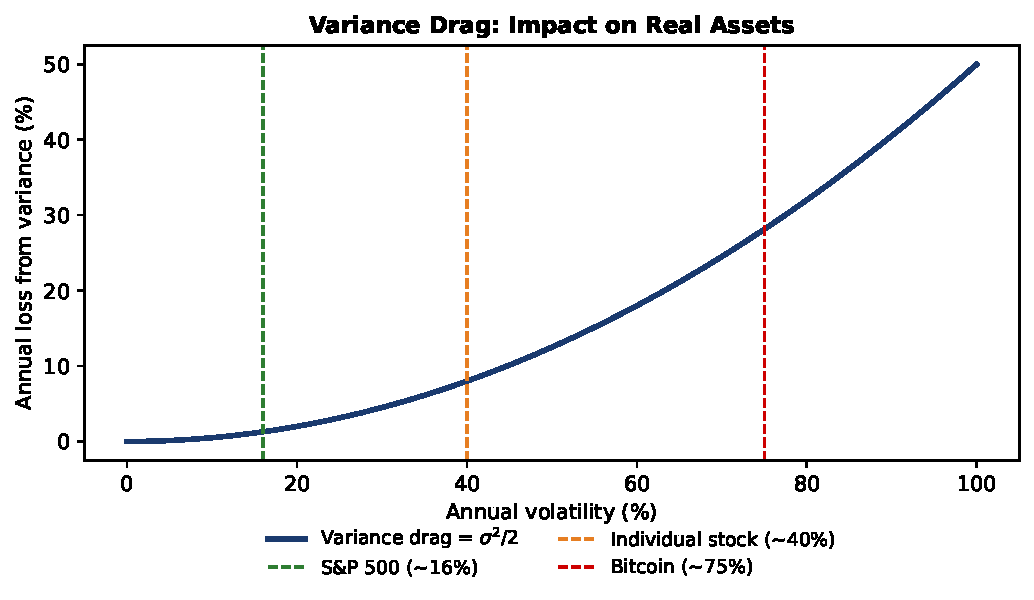
\includegraphics[width=0.82\linewidth]{sfm_ch1_variance_drag.pdf}
\end{center}
\vspace{-0.2cm}
\begin{itemize}\small\setlength{\itemsep}{1pt}
    \item Curba pierderii $\sigma^2/2$ este \textbf{cvadratică}: dublarea volatilității cvadruplează pierderea.
    \item S\&P 500 ($\sigma\approx16\%$): pierdere $\approx 1{,}3\%$/an; Bitcoin ($\sigma\approx75\%$): $\approx 28\%$/an.
\end{itemize}
\quantlet{SFM\_ch1\_variance\_drag}{https://github.com/QuantLet/Stat_fin_markets/tree/master/Ch_01/SFM_ch1_variance_drag}
\end{frame}

\begin{frame}{Randamente multi-perioadă și procesul de avuție}
\begin{defn}[Procesul de avuție]
\begin{itemize}\setlength{\itemsep}{1pt}
    \item Investind $W_0$ la momentul 0, avuția după $T$ perioade:
    $W_T = W_0 \prod_{t=1}^{T}(1 + R_t) = W_0\, \exp\!\bigl(\sum_{t=1}^T r_t\bigr).$
\end{itemize}
\end{defn}
\begin{itemize}\small\setlength{\itemsep}{1pt}
    \item \textbf{Log-wealth} este o sumă: $\ln W_T = \ln W_0 + \sum_{t=1}^T r_t$.
    \item Prin \textbf{Teorema Limită Centrală (TLC)}, $\ln W_T \approx$ normal pentru $T$ mare (dacă $r_t$ i.i.d.) $\Rightarrow$ $W_T$ este \textbf{log-normal}.
    \item Randamentul log pe $k$ perioade: $r_t(k) = \sum_{j=0}^{k-1} r_{t-j}$ (sumă, simplu).
    \item Randamentul simplu pe $k$ perioade: $R_t(k) = \prod_{j=0}^{k-1}(1+R_{t-j}) - 1$ (produs, mai dificil).
\end{itemize}
\begin{block}{Implicație practică}
\begin{itemize}
\item Pentru backtesting: sumați randamentele logaritmice, apoi convertiți la avuția finală prin $W_T = W_0 \cdot e^{\text{CLR}_T}$.
\end{itemize}
\end{block}
\end{frame}

\begin{frame}{Mișcarea browniană geometrică și proprietatea log-normală}
\begin{defn}[GBM --- Geometric Brownian Motion]
\begin{itemize}\setlength{\itemsep}{1pt}
    \item Modelul clasic Black-Scholes presupune că prețul urmează:
    $dP_t = \mu P_t\,dt + \sigma P_t\,dW_t,$
    cu soluția:
    \[
    P_T = P_0 \exp\!\Bigl[\bigl(\mu - \tfrac{\sigma^2}{2}\bigr)T + \sigma W_T\Bigr], \qquad W_T \sim \mathcal{N}(0, T).
    \]
\end{itemize}
\end{defn}
\begin{itemize}\small\setlength{\itemsep}{1pt}
    \item $\ln P_T \sim \mathcal{N}\!\bigl(\ln P_0 + (\mu - \sigma^2/2)T,\;\sigma^2 T\bigr)$ $\Rightarrow$ $P_T$ este \textbf{log-normal}.
    \item Termenul $-\sigma^2/2$ este \textbf{pierderea din varianță} (\textit{variance drag}): randamentul median $<$ randamentul mediu.
    \item \textbf{Legătură cu TLC}: pentru $r_t$ i.i.d., $\sum r_t \approx \mathcal{N}$ prin TLC $\Rightarrow$ $P_T$ log-normal.
\end{itemize}
\vspace{0.1cm}
\begin{alertblock}{Limitări ale GBM}
\begin{itemize}
\item \small GBM presupune volatilitate \textbf{constantă} și randamente \textbf{normal distribuite} --- ignoră cozi groase, gruparea volatilității și efectul de levier. Modelele GARCH și cu salturi (jump-diffusion) corectează aceste probleme.
\end{itemize}
\end{alertblock}
\end{frame}

\begin{frame}[shrink=3]{Randamente cumulate}
\begin{defn}[Randamente cumulate]
\begin{itemize}\setlength{\itemsep}{1pt}
    \item \textbf{CSR} (Randament simplu cumulat) de la 0 la $T$:
    $\text{CSR}_T = \prod_{t=1}^{T}(1+R_t) - 1.$
    \item \textbf{CLR} (Randament logaritmic cumulat) de la 0 la $T$:
    $\text{CLR}_T = \sum_{t=1}^{T} r_t = \ln\frac{P_T}{P_0}.$
    \item Relație: $\text{CSR}_T = e^{\text{CLR}_T} - 1$.
\end{itemize}
\end{defn}
\begin{itemize}
    \item CLR: sumă simplă, ușor de calculat.
    \item CSR: necesită compunere (înmulțire).
\end{itemize}
\vspace{-0.15cm}
\begin{center}
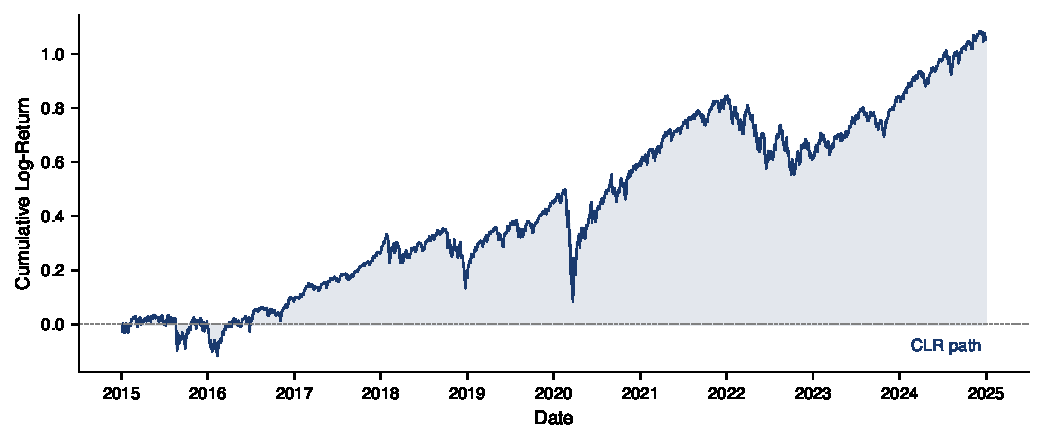
\includegraphics[width=0.55\linewidth]{sfm_ch1_cumulative.pdf}
\end{center}
\quantlet{SFM\_ch1\_returns\_analysis}{https://github.com/QuantLet/Stat_fin_markets/tree/master/Ch_01/SFM_ch1_returns_analysis}
\end{frame}

\begin{frame}{Randamente anualizate}
\begin{itemize}\small\setlength{\itemsep}{1pt}
    \item Pentru a compara strategiile pe diferite orizonturi, randamentele sunt \textbf{anualizate}.
    \item \textbf{Anualizare geometrică} (preferată; ține cont de compunere):
    $\bar{R}_{\text{annual}}^{\text{geo}} = \left(\prod_{t=1}^{T}(1+R_t)\right)^{252/T} - 1 = e^{\frac{252}{T}\cdot\text{CLR}_T} - 1.$
    \item \textbf{Anualizare aritmetică} (aproximare simplă):
    $\bar{R}_{\text{annual}}^{\text{arith}} = \frac{252}{T}\sum_{t=1}^{T} r_t.$
\end{itemize}
\vspace{0.05cm}
\begin{center}
{\footnotesize
\renewcommand{\arraystretch}{1.15}
\begin{tabular}{lcc}
\toprule
\textbf{Orizont} & \textbf{Factor geo.} & \textbf{Exemplu: medie 0,05\%/zi} \\
\midrule
Zilnic $\to$ Anual (252 zile) & $(1+\bar{R})^{252}-1$ & $(1.0005)^{252}-1 = 13.3\%$ \\
Lunar $\to$ Anual (12 luni) & $(1+\bar{R})^{12}-1$ & $(1.0105)^{12}-1 = 13.4\%$ \\
Trim.\ $\to$ Anual (4 trim.) & $(1+\bar{R})^{4}-1$ & $(1.0327)^{4}-1 = 13.8\%$ \\
\bottomrule
\end{tabular}
}
\end{center}
\vspace{0.05cm}
\begin{itemize}\small
    \item Randamentul aritmetic $>$ geometric cu aproximativ $\sigma^2/2$ per perioadă (pierderea din varianță).
\end{itemize}
\end{frame}

\begin{frame}{Momentele randamentelor}
\begin{itemize}
    \item \textbf{Media} (primul moment) --- randamentul așteptat:
    \[
    \mu = \E[r_t], \qquad \hat{\mu} = \frac{1}{n}\sum_{t=1}^n r_t.
    \]
    \item \textbf{Varianța} (al doilea moment central) --- risc total:
    \[
    \sigma^2 = \Var(r_t) = \E[(r_t-\mu)^2], \qquad \hat{\sigma}^2 = \frac{1}{n-1}\sum_{t=1}^n (r_t-\hat{\mu})^2.
    \]
    \item \textbf{Asimetria} (al treilea moment standardizat, \textit{skewness}):
    \[
    S = \frac{\E[(r_t-\mu)^3]}{\sigma^3}. \quad S<0 \Rightarrow \text{coadă stângă mai grea (mai multe pierderi mari).}
    \]
    \item \textbf{Kurtosis} (al patrulea moment standardizat):
    \[
    K = \frac{\E[(r_t-\mu)^4]}{\sigma^4}. \quad K>3 \Rightarrow \text{leptokurtic (cozi mai groase decât Distribuția Normală).}
    \]
    \item \textbf{Excess kurtosis}: $\kappa = K - 3$; Normal $\Rightarrow \kappa = 0$.
\end{itemize}
\end{frame}

\begin{frame}[shrink=3]{Asimetrie și kurtosis: Interpretare}
\begin{itemize}
    \item \textbf{Normal}: $S=0$, $K=3$.
    \item \textbf{Asimetrie stângă} ($S<0$): câștiguri mici frecvente, pierderi mari rare; tipic pentru \textit{indici bursieri}.
    \item \textbf{Cozi groase} ($K>3$): evenimente extreme mult mai probabile decât Distribuția Normală; universal în datele financiare.
    \item \textbf{Asimetrie dreaptă} ($S>0$): câștiguri mari ocazionale; tipic pentru opțiuni call OTM (\textit{out-of-the-money}).
\end{itemize}
\vspace{-0.15cm}
\begin{center}

\includegraphics[width=0.55\linewidth]{sfm_ch1_densities.pdf}
\end{center}
\quantlet{SFM\_ch1\_returns\_analysis}{https://github.com/QuantLet/Stat_fin_markets/tree/master/Ch_01/SFM_ch1_returns_analysis}
\end{frame}

\begin{frame}{Momente empirice: Exemplu}
\begin{itemize}
    \item Statistici eșantion pentru randamente logaritmice zilnice (aprox.\ 2015--2024):
\end{itemize}
\vspace{0.1cm}
\begin{center}
{\small
\renewcommand{\arraystretch}{1.3}
\begin{tabular}{lcccccc}
\toprule
\textbf{Activ} & \textbf{Medie} & \textbf{Std} & \textbf{Asimetrie} & \textbf{Kurtosis} & \textbf{Min} & \textbf{Max} \\
\midrule
S\&P 500 & $+0.040\%$ & $1.00\%$ & $-0.72$ & $12.1$ & $-12.8\%$ & $+9.4\%$ \\
AAPL     & $+0.058\%$ & $1.80\%$ & $-0.31$ & $8.6$  & $-13.0\%$ & $+11.9\%$ \\
Bitcoin  & $+0.195\%$ & $3.90\%$ & $-0.15$ & $7.4$  & $-46.5\%$ & $+22.5\%$ \\
EUR/USD  & $+0.000\%$ & $0.45\%$ & $+0.08$ & $5.2$  & $-2.7\%$  & $+3.1\%$ \\
\bottomrule
\end{tabular}
}
\end{center}
\vspace{0.1cm}
\begin{itemize}
    \item Toate activele: excess kurtosis $\gg 0$ (cozi groase confirmate).
    \item Acțiuni: asimetrie negativă (riscul de crah domină).
    \item BTC: volatilitate maximă; asimetrie negativă în ciuda narativului de asimetrie pozitivă.
    \item EUR/USD: medie aproape zero, aproape simetrică, dar cu cozi groase.
\end{itemize}
\quantlet{SFM\_ch1\_returns}{https://github.com/QuantLet/Stat_fin_markets/tree/master/Ch_01/SFM_ch1_returns}
\end{frame}

\begin{frame}[shrink=5]{Drawdown-uri}
\begin{defn}[Drawdown și MDD]
Drawdown la momentul $t$: $DD_t = \dfrac{P_t - \max_{s \leq t} P_s}{\max_{s \leq t} P_s} \leq 0$.
MDD: $\text{MDD} = \min_{t \in [0,T]} DD_t$.
\end{defn}
\vspace{0.05cm}
\begin{itemize}
    \item MDD: cel mai mare declin de la maxim la minim din istorie.
    \item Metric de risc cheie pentru strategiile de urmărire a tendinței.
    \item S\&P 500 MDD: $-56.8\%$ (Mar 2007--Mar 2009).
    \item BTC MDD: $-83\%$ (Dec 2017--Dec 2018).
    \item Calmar ratio: $\bar{R}_{\text{annual}} / |\text{MDD}|$.
\end{itemize}
\vspace{-0.15cm}
\begin{center}
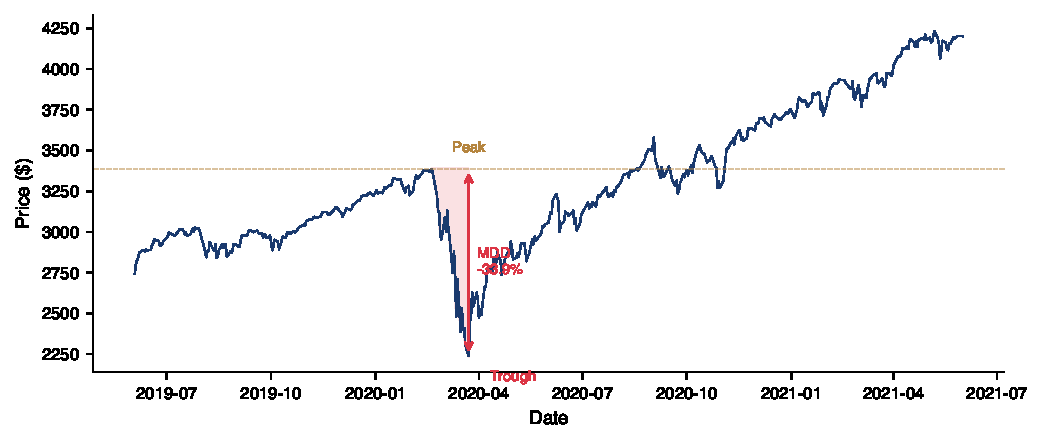
\includegraphics[width=0.55\linewidth]{sfm_ch1_drawdown.pdf}
\end{center}
\quantlet{SFM\_ch1\_returns\_analysis}{https://github.com/QuantLet/Stat_fin_markets/tree/master/Ch_01/SFM_ch1_returns_analysis}
\end{frame}

%=============================================================================
% ACTUALIZARE CUPRINS după Secțiunea 3
%=============================================================================
{
\setbeamertemplate{headline}{%
    \vskip10pt%
    \hbox to \paperwidth{\hskip0.5cm\hfill\hskip0.5cm}%
    \vskip4pt%
    {\color{FooterGray}\hrule height 0.4pt}%
}
\begin{frame}{}
    {\color{FooterGray}\hrule height 0.4pt}
    \vspace{0.1cm}
    {\Large\textcolor{IDAred}{\textbf{Cuprins}}}
    \vspace{0.2cm}
    \begin{enumerate}
        \item Motivație \checkmark
        \item Date de preț \checkmark
        \item Randamente \checkmark
        \item \textbf{Fapte stilizate ale randamentelor financiare}
        \item Estimatori de volatilitate
        \item Comparație de eficiență
        \item Randamente ajustate la risc
        \item Caz AI / Rezumat / Quiz
        \item Bibliografie
    \end{enumerate}
\end{frame}
}

%=============================================================================
% SECȚIUNEA 4: FAPTE STILIZATE
%=============================================================================
\section{Fapte stilizate}

\begin{frame}{Ipoteza pieței eficiente (EMH)}
\begin{defn}[Ipoteza pieței eficiente (Fama, 1970)]
\begin{itemize}\setlength{\itemsep}{1pt}
    \item O piață este \textbf{eficientă informațional} dacă prețurile \textit{reflectă complet} toată informația disponibilă.
    \item Trei forme:
\end{itemize}
\end{defn}
\vspace{0.1cm}
\begin{enumerate}
    \item \textbf{Forma slabă}: prețurile reflectă toate \textit{datele istorice de preț și volum}.\\
    $\Rightarrow$ Analiza tehnică nu poate genera randamente excesive; $\Corr(r_t, r_{t-k}) = 0$.
    \item \textbf{Forma semi-puternică}: prețurile reflectă toată \textit{informația publică disponibilă}.\\
    $\Rightarrow$ Analiza fundamentală nu poate genera randamente excesive; studiile de evenimente arată ajustare rapidă.
    \item \textbf{Forma puternică}: prețurile reflectă \textit{toată} informația (inclusiv privată/insider).\\
    $\Rightarrow$ Nici insiderii nu pot genera randamente excesive (încălcată empiric).
\end{enumerate}
\vspace{0.1cm}
\begin{itemize}
    \item Faptele stilizate de mai jos arată \textbf{unde EMH eșuează}: absența autocorelației liniare susține eficiența slabă, dar gruparea volatilității și efectul de levier sugerează momente de ordin doi predictibile.
\end{itemize}
\end{frame}

\begin{frame}{Fapte stilizate ale randamentelor financiare (\textit{stylized facts})}
\begin{itemize}
    \item Cont (2001) și Mandelbrot (1963) au identificat \textbf{regularități statistice universale} observate pe diferite piețe, instrumente și perioade de timp.
\end{itemize}
\vspace{0.15cm}
\begin{enumerate}
    \item \textbf{Absența autocorrelației liniare}: $\Corr(r_t, r_{t-k}) \approx 0$ pentru $k \geq 1$.
    \item \textbf{Cozi groase} (\textit{fat tails}): excess kurtosis $K > 3$ în distribuțiile randamentelor.
    \item \textbf{Asimetrie}: asimetrie negativă pentru randamentele acțiunilor.
    \item \textbf{Gruparea volatilității} (\textit{volatility clustering}): valorile mari ale $|r_t|$ tind să fie urmate de valori mari ale $|r_{t+1}|$.
    \item \textbf{Efectul de levier} (\textit{leverage effect}): randamentele negative cresc volatilitatea viitoare mai mult decât cele pozitive de aceeași magnitudine (Black, 1976).
    \item \textbf{Normalitate prin agregare} (aggregational Gaussianity): randamentele se apropie de normalitate pe măsură ce scala temporală crește.
    \item \textbf{Corelația volum-volatilitate}: volumul de tranzacționare și volatilitatea sunt corelate pozitiv.
\end{enumerate}
\end{frame}

\begin{frame}[shrink=10]{Cozi groase și non-normalitate}
\begin{itemize}\footnotesize\setlength{\itemsep}{0pt}
    \item Sub $\mathcal{N}(\mu,\sigma^2)$, un eveniment de $5\sigma$ are prob.\ $\approx 2.87 \times 10^{-7}$.
    \item \textbf{Black Monday} (19 Oct 1987): S\&P 500 $-22.6\%$ într-o zi ($>20\sigma$, prob.\ $\approx 10^{-89}$).
\end{itemize}
\vspace{0.05cm}
\begin{center}
{\footnotesize
\renewcommand{\arraystretch}{1.05}
\begin{tabular}{lcc}
\toprule
\textbf{Magnitudinea evenimentului} & \textbf{Prob.\ Normală} & \textbf{Frecvență observată} \\
\midrule
Mișcare $> 3\sigma$ & 0,27\% (1 la 370 zile) & $\sim$1 la 50--100 zile \\
Mișcare $> 4\sigma$ & 0,0063\% (1 la 16\,000 zile) & $\sim$1 la 500--1000 zile \\
Mișcare $> 5\sigma$ & 1 la 3,5 mil.\ zile & $\sim$1 la 5000--10\,000 zile \\
\bottomrule
\end{tabular}
}
\end{center}
\vspace{0.05cm}
\begin{alertblock}{Concluzie}
\begin{itemize}\small\setlength{\itemsep}{0pt}
    \item Randamentele sunt \textbf{leptokurtice}: Distribuția Normală subestimează dramatic riscul de coadă. Empiric $\approx$ Student-$t$ cu $\nu \in [4,8]$.
\end{itemize}
\end{alertblock}
\begin{exampleblock}{Implicație practică}
\begin{itemize}\small\setlength{\itemsep}{0pt}
    \item VaR-ul sub normalitate \textbf{subestimează} pierderile extreme. Un model Normal ar fi spus că Black Monday nu se poate întâmpla niciodată.
\end{itemize}
\end{exampleblock}
\end{frame}

\begin{frame}[shrink=3]{Cozi groase: Ilustrație QQ-Plot}
\begin{itemize}
    \item Un QQ-plot: cuantilele eșantionului vs.\ cuantilele distribuției normale.
    \item Dacă distribuția este Normală: punctele cad pe linia de 45$^\circ$ exact.
    \item \textbf{Formă de S}: coada stângă sub linie (pierderi mai extreme), coada dreaptă deasupra (câștiguri mai extreme).
    \item \textbf{Cozi groase}: ambele capete deviază în sus/jos față de linie.
    \item Testul Jarque-Bera: $JB = \frac{n}{6}(S^2 + \frac{\kappa^2}{4}) \sim \chi^2_2$ sub $H_0$.
    \item Testele Kolmogorov-Smirnov și Anderson-Darling sunt de asemenea folosite.
\end{itemize}
\vspace{-0.15cm}
\begin{center}
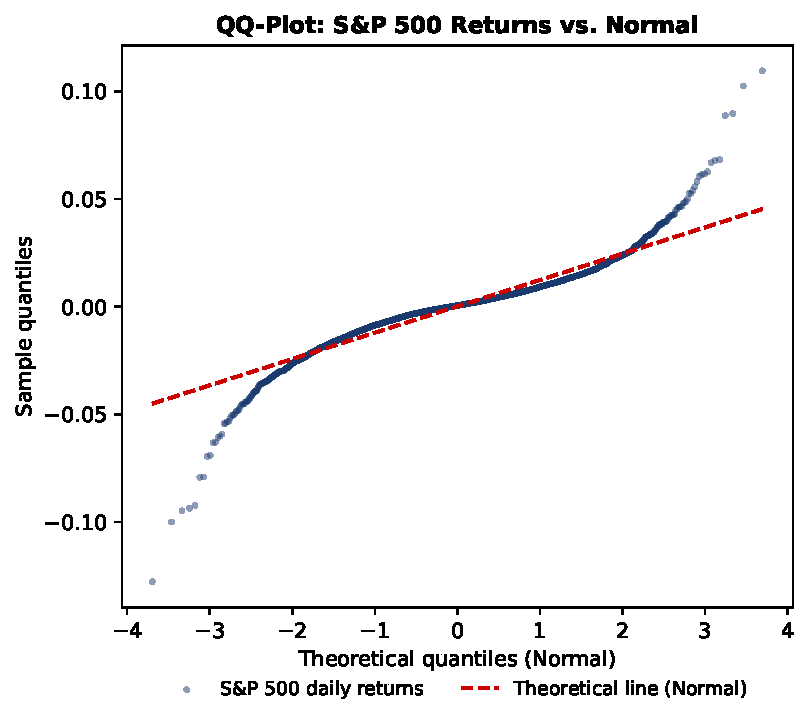
\includegraphics[width=0.55\linewidth]{sfm_ch1_qqplot.pdf}
\end{center}
\quantlet{SFM\_ch1\_stylized\_facts}{https://github.com/QuantLet/Stat_fin_markets/tree/master/Ch_01/SFM_ch1_stylized_facts}
\end{frame}

\begin{frame}{\mbox{Gruparea volatilității} (Volatility Clustering)}
\begin{itemize}\footnotesize\setlength{\itemsep}{0pt}
    \item Mandelbrot (1963): ``\textit{Schimbările mari tind să fie urmate de schimbări mari --- de orice semn --- iar schimbările mici tind să fie urmate de schimbări mici.}''
    \item Formal: $\Corr(r_t, r_{t-k}) \approx 0$ dar $\Corr(|r_t|, |r_{t-k}|) > 0$ pentru $k = 1, 2, \ldots$
\end{itemize}
\vspace{-0.15cm}
\begin{center}
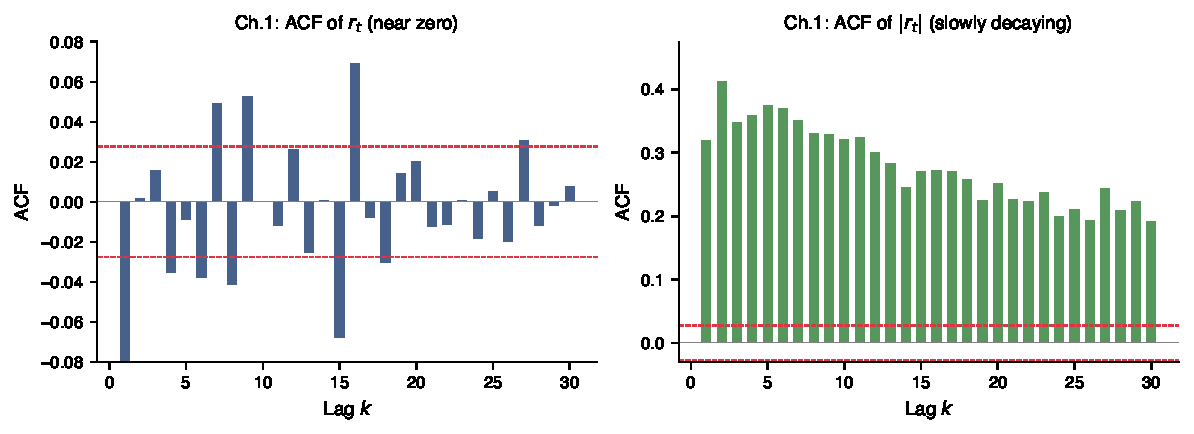
\includegraphics[width=0.62\linewidth]{sfm_ch1_acf.pdf}
\end{center}
\vspace{-0.3cm}
\begin{itemize}\footnotesize\setlength{\itemsep}{0pt}
    \item ACF a $|r_t|$: descreștere lentă (memorie lungă) $\Rightarrow$ motivează ARCH/GARCH.
    \item \textbf{Implicație}: \textit{„Volatilitatea este predictibilă, randamentele nu."}
\end{itemize}
\quantlet{SFM\_ch1\_stylized\_facts}{https://github.com/QuantLet/Stat_fin_markets/tree/master/Ch_01/SFM_ch1_stylized_facts}
\end{frame}

\begin{frame}{Efectul de levier (\textit{leverage effect})}
\begin{itemize}\footnotesize\setlength{\itemsep}{0pt}
    \item Black (1976): un randament \textit{negativ} crește volatilitatea viitoare \textit{mai mult} decât unul pozitiv de aceeași magnitudine.
    \item Când prețul scade, datoria/capital propriu $\uparrow$ $\Rightarrow$ risc mai mare.
    \item Formal: $\Corr(r_t, \sigma_{t+1}^2) < 0$.
\end{itemize}
\vspace{-0.15cm}
\begin{block}{GJR-GARCH(1,1)}
\vspace{-0.15cm}
{\small $\sigma_t^2 = \omega + (\alpha + \gamma\,\mathbf{1}_{r_{t-1}<0})\,r_{t-1}^2 + \beta\,\sigma_{t-1}^2$}
\vspace{-0.1cm}
\end{block}
\vspace{-0.15cm}
\begin{center}
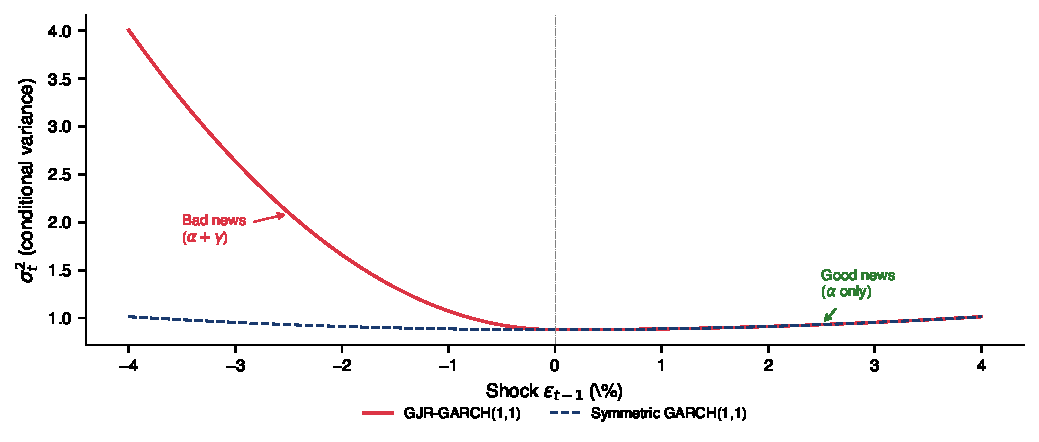
\includegraphics[width=0.55\linewidth]{sfm_ch1_leverage.pdf}
\end{center}
\quantlet{SFM\_ch1\_leverage\_effect}{https://github.com/QuantLet/Stat_fin_markets/tree/master/Ch_01/SFM_ch1_leverage_effect}
\end{frame}

\begin{frame}{Teorema Limită Centrală (TLC)}
\begin{thm}[Teorema Limită Centrală]
Fie $X_1, X_2, \ldots, X_n$ variabile aleatoare i.i.d.\ cu $\E[X_i] = \mu$ și $\Var(X_i) = \sigma^2 < \infty$. Atunci:
\[
\frac{\bar{X}_n - \mu}{\sigma / \sqrt{n}} \xrightarrow{d} \mathcal{N}(0, 1) \quad \text{când } n \to \infty.
\]
\end{thm}
\vspace{0.1cm}
\begin{itemize}
    \item \textbf{Intuiție}: suma (sau media) unui număr mare de variabile aleatoare independente tinde spre Distribuția Normală, \textit{indiferent} de distribuția originală.
    \item \textbf{Condiție cheie}: varianța finită ($\sigma^2 < \infty$). Eșuează pentru distribuții Pareto-stabile ($\alpha < 2$).
    \item \textbf{Viteză de convergență} (Berry-Esseen): $\sup_x |F_n(x) - \Phi(x)| \leq \frac{C\,\E[|X_1 - \mu|^3]}{\sigma^3\sqrt{n}}$, cu $C \leq 0.4748$.
    \item \textbf{Relevanță financiară}: randamentele pe $k$ zile $= \sum_{j=1}^{k}r_j$ --- TLC justifică aproximarea normală pentru orizonturi mai lungi.
\end{itemize}
\end{frame}

\begin{frame}{TLC: Convergența vizuală}
\begin{center}

\includegraphics[width=0.85\linewidth]{sfm_ch1_clt.pdf}
\end{center}
\vspace{-0.2cm}
\begin{itemize}\small
    \item Pe măsură ce $n$ crește, distribuția sumelor standardizate se apropie de curba normală (linia roșie), indiferent de distribuția inițială.
\end{itemize}
\end{frame}

\begin{frame}[shrink=3]{Normalitate prin agregare (aggregational Gaussianity)}
\begin{itemize}
    \item \textbf{Zilnic}: cozi foarte groase, excess kurtosis $\approx 5$--$20$.
    \item \textbf{Săptămânal}: kurtosis redus, mai puține valori aberante extreme.
    \item \textbf{Lunar}: aproximativ normală prin Teorema Limită Centrală (TLC).
    \item TLC: $r_t^{(k)} = \sum_{j=0}^{k-1}r_{t-j} \xrightarrow{d} \mathcal{N}$ când $k\to\infty$, sub condiții slabe ($\sigma^2 < \infty$).
    \item \textbf{Caveat}:
    \begin{itemize}
        \item Convergența este \textit{lentă} pentru distribuțiile Pareto-stabile
        \item Distribuțiile cu varianță infinită nu converg niciodată la Distribuția Normală
    \end{itemize}
\end{itemize}
\vspace{-0.15cm}
\begin{center}
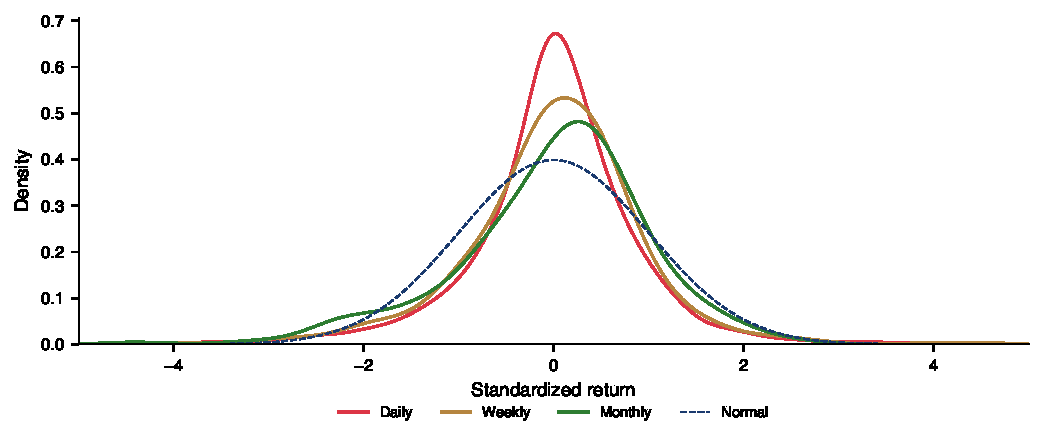
\includegraphics[width=0.55\linewidth]{sfm_ch1_aggregation.pdf}
\end{center}
\quantlet{SFM\_ch1\_stylized\_facts}{https://github.com/QuantLet/Stat_fin_markets/tree/master/Ch_01/SFM_ch1_stylized_facts}
\end{frame}

\begin{frame}{Corelația volum-volatilitate}
\begin{itemize}
    \item \textbf{Fapt empiric}: volumul $V_t$ și $|r_t|$ sunt corelate pozitiv.
    \item \textbf{MDH} (\textit{Mixture of Distributions Hypothesis}, Clark 1973; Tauchen \& Pitts 1983): ambele determinate de fluxul informațional latent.
    \item \textbf{Sosire secvențială} (Copeland 1976): traderii învață secvențial.
    \item Modelele GARCH augmentate cu volum depășesc GARCH standard.
\end{itemize}
\vspace{-0.15cm}
\begin{center}
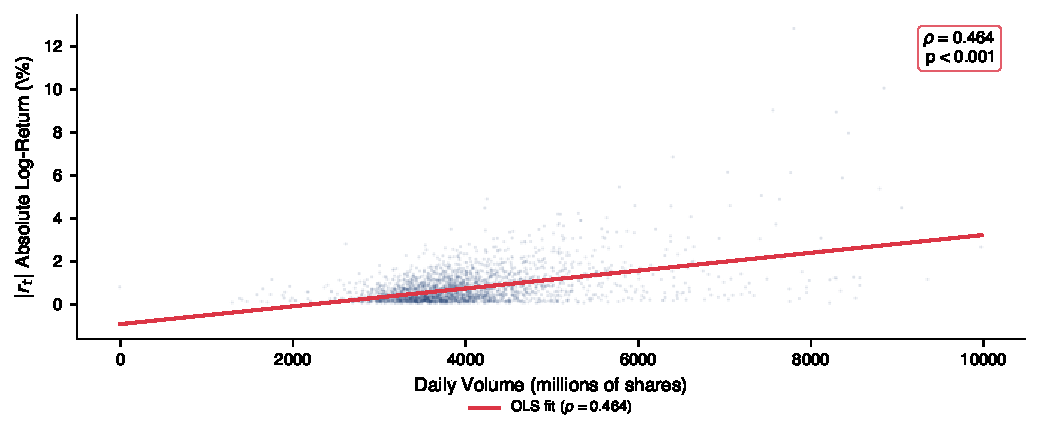
\includegraphics[width=0.55\linewidth]{sfm_ch1_volume_vol.pdf}
\end{center}
\quantlet{SFM\_ch1\_volume\_volatility}{https://github.com/QuantLet/Stat_fin_markets/tree/master/Ch_01/SFM_ch1_volume_volatility}
\end{frame}

\begin{frame}{De la fapte stilizate la modele}
\begin{center}
{\small
\renewcommand{\arraystretch}{1.3}
\begin{tabular}{>{\bfseries}lll}
\toprule
\textbf{Fapt stilizat} & \textbf{Implicație pentru modelare} & \textbf{Capitol} \\
\midrule
Cozi groase (fat tails) & Distribuția Student-$t$, stable Paretian & Cap.\ 2 \\
Gruparea volatilității & GARCH, EGARCH & Cap.\ 5 \\
Efect de levier & GJR-GARCH, EGARCH asimetric & Cap.\ 5 \\
Absența autocorelației în $r_t$ & EMH forma slabă; randamente $\approx$ MDS & Cap.\ 3 \\
Autocorelație în $|r_t|$ și $r_t^2$ & Memorie lungă, FIGARCH & Cap.\ 5 \\
Normalitate prin agregare & TLC; modele cu varianță finită & Cap.\ 2 \\
Corelație volum-volatilitate & MDH, modele GARCH cu volum & Cap.\ 5 \\
\bottomrule
\end{tabular}
}
\end{center}
\vspace{0.1cm}
\begin{block}{Concluzie}
\begin{itemize}
\item \small Faptele stilizate nu sunt doar curiozități empirice --- ele \textbf{ghidează} alegerea modelului statistic. Un model bun trebuie să reproducă aceste regularități.
\end{itemize}
\end{block}
\end{frame}

%=============================================================================
% SFÂRȘITUL PĂRȚII I --- pauză sugerată între lecții
%=============================================================================
% Dacă se livrează pe două sesiuni:
%   Partea I  (Secțiunile 1--4): Date, Randamente, Fapte stilizate
%   Partea II (Secțiunile 5--8): Estimatori de volatilitate, Eficiență, Randamente ajustate la risc
%=============================================================================

%=============================================================================
% ACTUALIZARE CUPRINS după Secțiunea 4
%=============================================================================
{
\setbeamertemplate{headline}{%
    \vskip10pt%
    \hbox to \paperwidth{\hskip0.5cm\hfill\hskip0.5cm}%
    \vskip4pt%
    {\color{FooterGray}\hrule height 0.4pt}%
}
\begin{frame}{}
    {\color{FooterGray}\hrule height 0.4pt}
    \vspace{0.1cm}
    {\Large\textcolor{IDAred}{\textbf{Cuprins}}}
    \vspace{0.2cm}
    \begin{enumerate}
        \item Motivație \checkmark
        \item Date de preț \checkmark
        \item Randamente \checkmark
        \item Fapte stilizate ale randamentelor financiare \checkmark
        \item \textbf{Estimatori de volatilitate}
        \item Comparație de eficiență
        \item Randamente ajustate la risc
        \item Caz AI / Rezumat / Quiz
        \item Bibliografie
    \end{enumerate}
\end{frame}
}

%=============================================================================
% TITLU PARTEA II
%=============================================================================
{
\setbeamertemplate{headline}{}
\setbeamertemplate{footline}{}
\begin{frame}[plain]
\vfill
\begin{center}
{\Huge\textcolor{IDAred}{\textbf{Partea II}}}

\vspace{0.6cm}

{\Large\textcolor{MainBlue}{Estimatori de Volatilitate, Eficiență și Performanță}}

\vspace{0.4cm}

{\large\textcolor{MediumGray}{--- Secțiunile 5--8 ---}}
\end{center}
\vfill
\end{frame}
}

%=============================================================================
% SECȚIUNEA 5: ESTIMATORI DE VOLATILITATE
%=============================================================================
\section{Estimatori de volatilitate}

\begin{frame}{Volatilitatea: Conceptul central}
\begin{defn}[Volatilitate]
\begin{itemize}\setlength{\itemsep}{1pt}
    \item Gradul de variație al unei serii de prețuri de tranzacționare în timp
    \item Măsurată prin \textbf{abaterea standard} (sau varianța) randamentelor
    \item Este o \textbf{variabilă latentă}: neobservabilă direct, doar estimabilă
\end{itemize}
\end{defn}
\vspace{0.1cm}
\begin{center}
{\scriptsize
\renewcommand{\arraystretch}{1.3}
\begin{tabular}{llll}
\toprule
\textbf{Estimator} & \textbf{Date utilizate} & \textbf{RE vs.\ CC} & \textbf{Referință cheie} \\
\midrule
Close-to-Close (CC) & doar $C_t$ & 1.0 & Statistică clasică \\
Parkinson (P) & $H_t, L_t$ & 5.2 & Parkinson (1980) \\
Garman-Klass (GK) & $O_t,H_t,L_t,C_t$ & 7.4 & Garman \& Klass (1980) \\
Rogers-Satchell (RS) & $O_t,H_t,L_t,C_t$ & 8.0 & Rogers \& Satchell (1991) \\
Yang-Zhang (YZ) & $O_t,H_t,L_t,C_t$ & 14.0 & Yang \& Zhang (2000) \\
Realized Vol (RV) & Tick-uri intra-zilnice & $\gg$14 & Andersen \& Bollerslev (1998) \\
\bottomrule
\end{tabular}
}
\end{center}
\end{frame}

\begin{frame}{Tipuri de volatilitate: Taxonomie}
\begin{center}
{\footnotesize
\renewcommand{\arraystretch}{1.3}
\begin{tabular}{>{\bfseries}lllll}
\toprule
\textbf{Tip} & \textbf{Sursa datelor} & \textbf{Ce măsoară} & \textbf{Când folosim} & \textbf{Exemplu} \\
\midrule
Istorică & Prețuri trecute & Vol.\ medie pe & Evaluare pe & CC, rolling \\
(necondițională) & ($C_t$ sau OHLC) & termen lung & termen lung & 252 zile \\
\midrule
Condițională & Randamente + & Vol.\ variabilă & Risc pe & GARCH, \\
 & model & în timp & termen scurt & EWMA \\
\midrule
Realizată & Randamente & Vol.\ zilnică & Benchmark & RV cu date \\
 & intrazilnice & reală & de aur & la 5 min \\
\midrule
Implicită & Prețuri & Așteptarea & Tranzacționare & VIX, \\
 & de opțiuni & pieței & opțiuni & IV surface \\
\bottomrule
\end{tabular}
}
\end{center}
\vspace{0.05cm}
\begin{alertblock}{De reținut}
\begin{itemize}\setlength{\itemsep}{0pt}
    \item Volatilitatea istorică privește \textbf{în trecut}, cea condițională estimează \textbf{azi}, cea implicită estimează \textbf{viitorul}. Fiecare răspunde la o altă întrebare.
\end{itemize}
\end{alertblock}
\end{frame}

\begin{frame}{Volatilitate istorică (Estimatorul Close-to-Close)}
\begin{defn}[Volatilitate istorică]
\begin{itemize}\setlength{\itemsep}{1pt}
    \item Estimatorul standard bazat pe $n$ randamente logaritmice:
    \[
    \hat{\sigma}_{\text{CC}} = \sqrt{\frac{1}{n-1}\sum_{t=1}^{n}(r_t - \bar{r})^2}, \qquad \bar{r} = \frac{1}{n}\sum_{t=1}^n r_t.
    \]
\end{itemize}
\end{defn}
\begin{itemize}
    \item Aceasta este pur și simplu abaterea standard eșantion a randamentelor logaritmice.
    \item \textbf{Anualizare}: $\hat{\sigma}_{\text{annual}} = \hat{\sigma}_{\text{daily}} \times \sqrt{252}$.
    \item \textbf{Avantaje}: simplu, intuitiv, necesită doar prețuri de închidere.
    \item \textbf{Limitări}: ignoră informațiile intra-zilnice (O, H, L); ponderează egal toate observațiile; sensibil la lungimea ferestrei $n$; întârzie schimbările de regim.
\end{itemize}
\quantlet{SFM\_ch1\_volatility\_estimators}{https://github.com/QuantLet/Stat_fin_markets/tree/master/Ch_01/SFM_ch1_volatility_estimators}
\end{frame}

\begin{frame}{Volatilitate istorică: Estimare rolling}
\vspace{-0.2cm}
\begin{itemize}\footnotesize\setlength{\itemsep}{0pt}
    \item O \textbf{fereastră glisantă} de $n$ zile oferă o estimare a volatilității variabilă în timp.
    \item Alegeri uzuale: $n = 20$ zile (termen scurt), $n = 60$ zile (termen mediu).
\end{itemize}
\vspace{-0.2cm}
\begin{center}
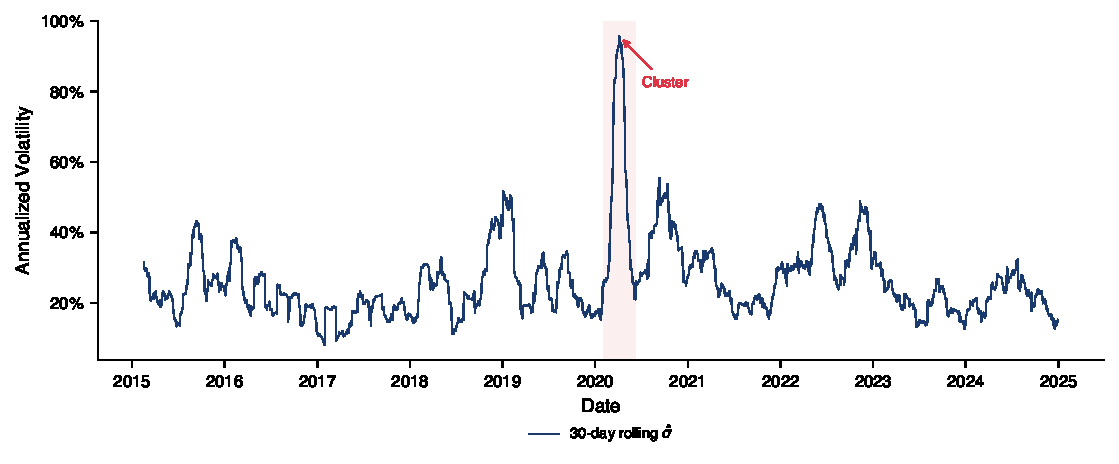
\includegraphics[width=0.65\linewidth]{sfm_ch1_rolling_vol.pdf}
\end{center}
\vspace{-0.3cm}
\begin{itemize}\footnotesize\setlength{\itemsep}{0pt}
    \item Clusterele de volatilitate sunt clar vizibile în estimările rolling.
    \item Lungimea ferestrei: scurtă $\to$ zgomotoasă; lungă $\to$ depășită.
\end{itemize}
\quantlet{SFM\_ch1\_volatility\_charts}{https://github.com/QuantLet/Stat_fin_markets/tree/master/Ch_01/SFM_ch1_volatility_charts}
\end{frame}

\begin{frame}[shrink=3]{Regula rădăcinii pătrate a timpului (\textit{Square Root of Time Rule})}
\begin{thm}
Dacă $r_1, r_2, \ldots$ sunt i.i.d.\ cu $\Var(r_t) = \sigma_1^2$, atunci $\sigma_T = \sigma_1 \sqrt{T}.$
\end{thm}
\vspace{-0.15cm}
\begin{itemize}\footnotesize\setlength{\itemsep}{0pt}
    \item \textbf{Dem.}\; $\Var(\sum_{t=1}^T r_t) = T\sigma_1^2 \Rightarrow \text{SD} = \sigma_1\sqrt{T}$.\hfill$\square$
    \item \textbf{Scalare}: $\sigma_{\text{annual}} = \sigma_{\text{daily}} \!\times\! \sqrt{252}$;\; $\sigma_{\text{monthly}} = \sigma_{\text{daily}} \!\times\! \sqrt{22}$;\; $\sigma_{\text{weekly}} = \sigma_{\text{daily}} \!\times\! \sqrt{5}$.
\end{itemize}
\vspace{0.02cm}
\begin{alertblock}{Când eșuează regula?}
\footnotesize
Presupune randamente necorelate cu varianță finită. Eșuează când:
\begin{itemize}\setlength{\itemsep}{0pt}
    \item Randamente \textbf{autocorelate} ($\rho > 0$ $\Rightarrow$ vol reală $>$ estimare)
    \item Volatilitate \textbf{variabilă în timp} (efecte GARCH)
    \item \textbf{Varianță infinită} (stable Paretian)
\end{itemize}
\end{alertblock}
\end{frame}

\begin{frame}[shrink=10]{Rădăcina pătrată a timpului: Exemplu numeric}
\begin{example}
Volatilitatea zilnică $\hat{\sigma}_{\text{daily}} = 1.2\%$.
\end{example}
\vspace{0.05cm}
\begin{center}
{\footnotesize
\renewcommand{\arraystretch}{1.15}
\begin{tabular}{lcl}
\toprule
\textbf{Orizont} & $\sqrt{T}$ & \textbf{Vol} \\
\midrule
1 zi    & $1.0$   & $1.2\%$ \\
1 săpt. & $2.2$   & $2.7\%$ \\
1 lună  & $4.7$   & $5.6\%$ \\
1 trim. & $7.9$   & $9.5\%$ \\
1 an    & $15.9$  & $19.1\%$ \\
\bottomrule
\end{tabular}
}
\end{center}
\vspace{-0.1cm}
\begin{itemize}
    \item Cu autocorelație AR(1) $\rho > 0$: $\sigma_T^2 = T\sigma_1^2\!\left[1 + 2\sum_{k=1}^{T-1}(1-k/T)\rho^k\right] > T\sigma_1^2$.
\end{itemize}
\vspace{-0.15cm}
\begin{center}
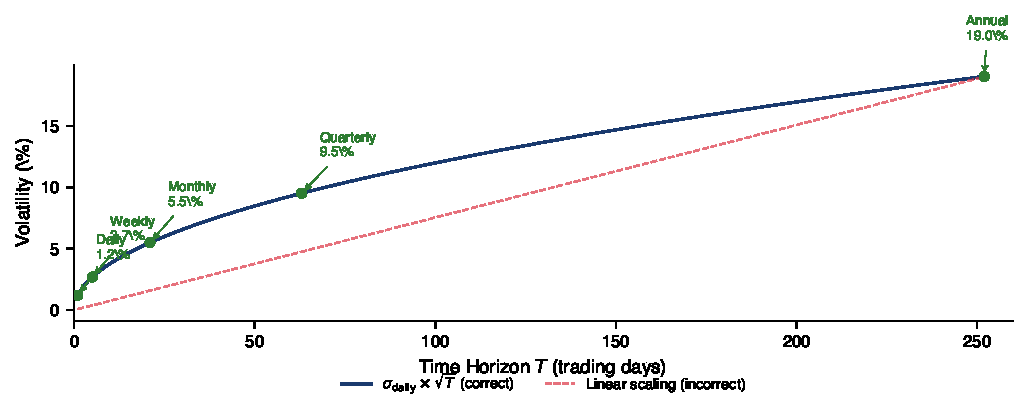
\includegraphics[width=0.55\linewidth]{sfm_ch1_sqrt_time.pdf}
\end{center}
\quantlet{SFM\_ch1\_vol\_comparison}{https://github.com/QuantLet/Stat_fin_markets/tree/master/Ch_01/SFM_ch1_vol_comparison}
\end{frame}

\begin{frame}{Mini-exercițiu: Anualizarea volatilității}
\begin{exampleblock}{Exercițiu pe slide}
Dacă $\sigma_{\text{daily}} = 1.5\%$, calculați:
\begin{enumerate}\setlength{\itemsep}{0pt}
    \item $\sigma_{\text{weekly}}$ (5 zile) $= ?$
    \item $\sigma_{\text{monthly}}$ (22 zile) $= ?$
    \item $\sigma_{\text{annual}}$ (252 zile) $= ?$
\end{enumerate}
\end{exampleblock}
\vspace{0.1cm}
\begin{block}{Rezolvare}
\begin{enumerate}\setlength{\itemsep}{0pt}
    \item $\sigma_{\text{weekly}} = 1.5\% \times \sqrt{5} = 1.5\% \times 2.236 = \mathbf{3.35\%}$
    \item $\sigma_{\text{monthly}} = 1.5\% \times \sqrt{22} = 1.5\% \times 4.690 = \mathbf{7.04\%}$
    \item $\sigma_{\text{annual}} = 1.5\% \times \sqrt{252} = 1.5\% \times 15.875 = \mathbf{23.81\%}$
\end{enumerate}
\end{block}
\vspace{0.05cm}
\begin{alertblock}{Atenție}
\begin{itemize}\setlength{\itemsep}{0pt}
\item Aceste calcule presupun randamente i.i.d. --- validați mereu ipoteza înainte de a aplica regula $\sqrt{T}$.
\end{itemize}
\end{alertblock}
\end{frame}

\begin{frame}[shrink=3]{Estimatorul Parkinson (1980)}
\begin{defn}[Estimatorul Parkinson]
\begin{itemize}\setlength{\itemsep}{1pt}
    \item Utilizând doar prețurile maxim și minim:
    \[
    \hat{\sigma}_{\text{P}}^2 = \frac{1}{4n\ln 2}\sum_{t=1}^{n}\left(\ln\frac{H_t}{L_t}\right)^2.
    \]
\end{itemize}
\end{defn}
\begin{itemize}
    \item \textbf{Derivare.} Sub GBM (\textit{Geometric Brownian Motion}) cu $\mu=0$: $\E[(\ln H/L)^2] = 4\sigma^2\ln 2$, deci $1/(4\ln 2) \approx 0.361$.
\end{itemize}
\vspace{0.05cm}
\begin{columns}[T]
\begin{column}{0.48\textwidth}
\begin{block}{Avantaje}
\begin{itemize}\setlength{\itemsep}{0pt}
    \item $5{,}2\times$ mai eficient decât CC
    \item Utilizează informația de range intraday
    \item Formulă simplă, ușor de calculat
\end{itemize}
\end{block}
\end{column}
\begin{column}{0.48\textwidth}
\begin{block}{Limitări}
\begin{itemize}\setlength{\itemsep}{0pt}
    \item Presupune GBM cu drift zero
    \item Presupune tranzacționare continuă (fără salturi)
    \item Distorsionată în jos dacă H/L reale nu sunt observate
\end{itemize}
\end{block}
\end{column}
\end{columns}
\end{frame}

\begin{frame}{Estimatorul Garman-Klass (1980)}
\begin{defn}[Estimatorul Garman-Klass]
\begin{itemize}\setlength{\itemsep}{1pt}
    \item Utilizând toate cele patru prețuri OHLC (GBM cu drift zero):
    {\small
    \[
    \hat{\sigma}_{\text{GK}}^2 = \frac{1}{n}\sum_{t=1}^{n}\!\left[0.5\!\left(\ln\frac{H_t}{L_t}\right)^{\!2} - (2\ln 2 - 1)\!\left(\ln\frac{C_t}{O_t}\right)^{\!2}\right].
    \]
    }
\end{itemize}
\end{defn}
\begin{itemize}
    \item \textbf{Derivare}: descompune varianța totală în componentele interval (\textit{range}) + închidere-deschidere; minimizează varianța estimatorului.
    \item \textbf{Eficiență}: $\approx 7.4\times$ mai eficient decât CC.
    \item \textbf{Limitare}: presupune $\mu=0$; distorsionată pe piețe în trend.
\end{itemize}
\begin{columns}[T]
\begin{column}{0.48\textwidth}
\begin{block}{Avantaje}
\begin{itemize}\setlength{\itemsep}{0pt}
    \item Cea mai bună eficiență cu drift zero
    \item Utilizează informația de range și O-to-C
\end{itemize}
\end{block}
\end{column}
\begin{column}{0.48\textwidth}
\begin{block}{Limitări}
\begin{itemize}\setlength{\itemsep}{0pt}
    \item Distorsionată pe piețe cu trend
    \item Gap-urile overnight introduc bias
\end{itemize}
\end{block}
\end{column}
\end{columns}
\end{frame}

\begin{frame}{Estimatorul Rogers-Satchell (1991)}
\begin{defn}[Estimatorul Rogers-Satchell]
\begin{itemize}\setlength{\itemsep}{1pt}
    \item Estimatorul RS \textbf{permite drift nenul}:
    {\small
    \[
    \hat{\sigma}_{\text{RS}}^2 = \frac{1}{n}\sum_{t=1}^{n}\!\left[\ln\frac{H_t}{C_t}\cdot\ln\frac{H_t}{O_t} + \ln\frac{L_t}{C_t}\cdot\ln\frac{L_t}{O_t}\right].
    \]
    }
\end{itemize}
\end{defn}
\begin{columns}[T]
\begin{column}{0.48\textwidth}
\begin{block}{Proprietăți cheie}
\begin{itemize}\setlength{\itemsep}{0pt}
    \item \textbf{Independent de drift}: nedeplasată cu $\mu\neq0$
    \item Performanță bună pe piețe cu trend
    \item $\approx 8\times$ mai eficient decât CC
\end{itemize}
\end{block}
\end{column}
\begin{column}{0.48\textwidth}
\begin{block}{Aplicații}
\begin{itemize}\setlength{\itemsep}{0pt}
    \item Piețe emergente (\"{O}zt\"{u}rk et al., 2016)
    \item Criptomonede (Cadenas-Morales, 2022)
    \item \textbf{Presupune}: tranzacționare continuă, fără salturi
\end{itemize}
\end{block}
\end{column}
\end{columns}
\end{frame}

\begin{frame}{Estimatorul Yang-Zhang (2000)}
\begin{defn}[Estimatorul Yang-Zhang]
\begin{itemize}\setlength{\itemsep}{1pt}
    \item Combină componentele overnight, open-to-close și Rogers-Satchell:
    $\hat{\sigma}_{\text{YZ}} = \sqrt{\hat{\sigma}_O^2 + k\,\hat{\sigma}_C^2 + (1-k)\,\hat{\sigma}_{\text{RS}}^2}$
    \item $\alpha = 1.34$ constanta optimală (Yang \& Zhang, 2000)
    \item $k = (\alpha-1)\big/\bigl(\alpha + (T+1)/(T-1)\bigr) \approx 0.34$ pentru $T$ tipic
\end{itemize}
\end{defn}
\vspace{0.05cm}
\begin{itemize}
    \item $\hat{\sigma}_O^2$: \textbf{overnight variance} $= \frac{1}{T-1}\sum_{t=1}^{T}\!\left(\ln\frac{O_t}{C_{t-1}} - \overline{\ln\frac{O_t}{C_{t-1}}}\right)^{\!2}$.
    \item $\hat{\sigma}_C^2$: \textbf{open-to-close variance} $= \frac{1}{T-1}\sum_{t=1}^{T}\!\left(\ln\frac{C_t}{O_t} - \overline{\ln\frac{C_t}{O_t}}\right)^{\!2}$.
    \item $\hat{\sigma}_{\text{RS}}^2$: componenta Rogers-Satchell.
    \item \textbf{$14\times$ mai eficient} decât CC; gestionează drift și salturi overnight.
    \item Cel mai bun estimator general pentru date OHLC zilnice.
\end{itemize}
\end{frame}

\begin{frame}{Estimatori de volatilitate: Comparație vizuală (AAPL 2018--2024)}
\vspace{-0.15cm}
\begin{center}
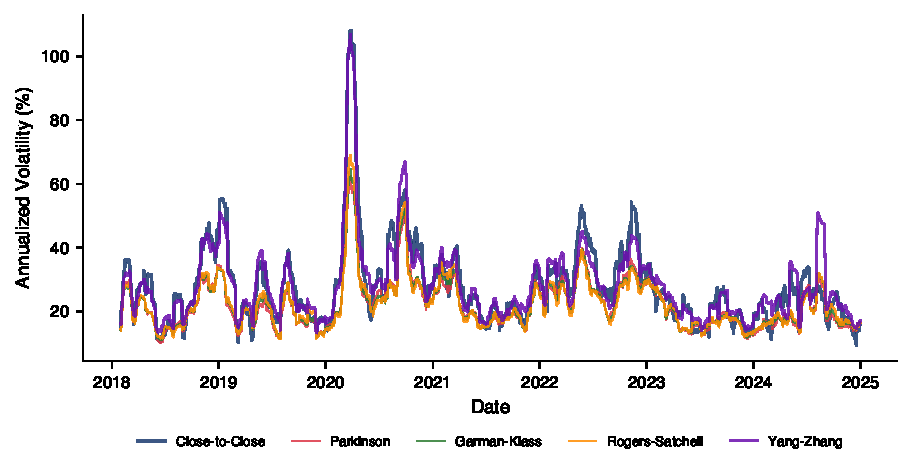
\includegraphics[width=0.76\linewidth]{sfm_ch1_vol_estimators_ts.pdf}
\end{center}
\vspace{-0.3cm}
\begin{itemize}\footnotesize\setlength{\itemsep}{0pt}
    \item Range-based (P, GK, RS) sunt mai netezi decât CC; YZ combină overnight + intraday.
    \item În criză (2020) toate captează vârful, dar cu magnitudini diferite.
\end{itemize}
\quantlet{SFM\_ch1\_volatility\_estimators}{https://github.com/QuantLet/Stat_fin_markets/tree/master/Ch_01/SFM_ch1_volatility_estimators}
\end{frame}

\begin{frame}{Estimatori de volatilitate: Comparație numerică (AAPL 2020--2024)}
\vspace{-0.1cm}
\begin{center}
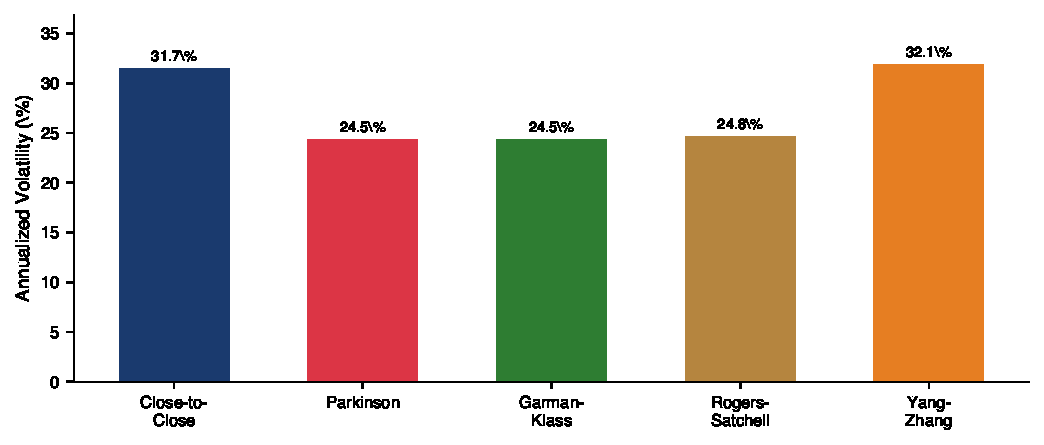
\includegraphics[width=0.80\linewidth]{sfm_ch1_vol_comparison.pdf}
\end{center}
\vspace{-0.3cm}
\begin{itemize}\footnotesize\setlength{\itemsep}{0pt}
    \item Range-based (P, GK, RS) produc volatilitate \textbf{mai mică} decât CC --- extrag mai multă informație.
    \item YZ combină overnight + intraday; diferențele cresc pe piețe volatile cu gap-uri mari.
\end{itemize}
\quantlet{SFM\_ch1\_vol\_comparison}{https://github.com/QuantLet/Stat_fin_markets/tree/master/Ch_01/SFM_ch1_vol_comparison}
\end{frame}

\begin{frame}{Volatilitatea EWMA}
\begin{itemize}
    \item {\small $\hat{\sigma}_t^2 = \lambda\,\hat{\sigma}_{t-1}^2 + (1-\lambda)\,r_{t-1}^2$, \quad $\lambda = 0.94$.}
    \item Ponderea la lag-ul $k$: $(1-\lambda)\lambda^k$ (descreștere exponențială).
    \item $\lambda=0.94$: fereastră efectivă $\approx 16{,}7$ zile.
    \item \textbf{Avantaje}: reacționează rapid; fără fereastră fixă; ușor de actualizat.
    \item \textbf{Dezavantaje}: fără revenire la medie; $\lambda$ stabilit extern.
\end{itemize}
\vspace{-0.15cm}
\begin{center}
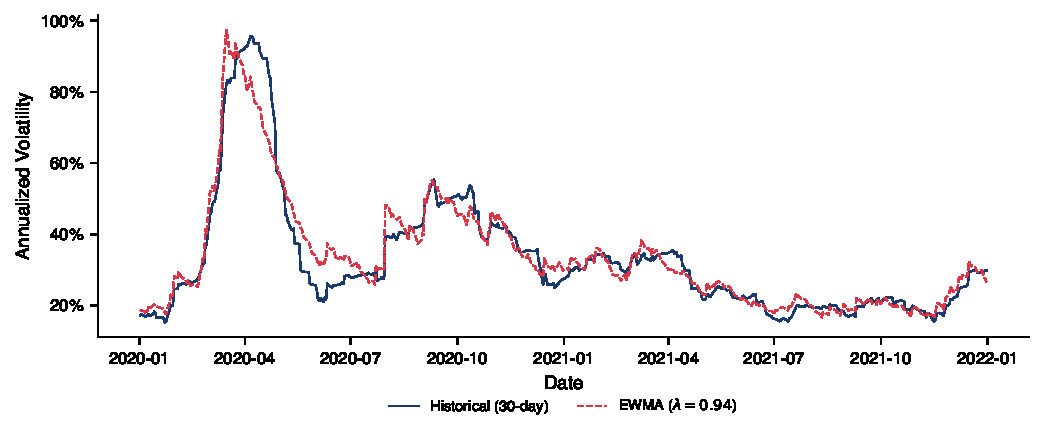
\includegraphics[width=0.55\linewidth]{sfm_ch1_ewma.pdf}
\end{center}
\quantlet{SFM\_ch1\_volatility\_charts}{https://github.com/QuantLet/Stat_fin_markets/tree/master/Ch_01/SFM_ch1_volatility_charts}
\end{frame}

\begin{frame}{Volatilitatea realizată}
\begin{defn}[Volatilitate realizată]
\begin{itemize}\setlength{\itemsep}{1pt}
    \item Date fiind $m$ randamente logaritmice intrazilnice la frecvența $\Delta = 1/m$:
    \[
    \text{RV}_t = \sum_{j=1}^{m} r_{t,j}^2, \qquad r_{t,j} = \ln P_{t,j} - \ln P_{t,j-1}.
    \]
\end{itemize}
\end{defn}
\begin{itemize}
    \item \textbf{Consistență}: $\text{RV}_t \xrightarrow{p} \int_0^1 \sigma_t^2(s)\,ds$ când $m \to \infty$ (Andersen \& Bollerslev, 1998).
    \item În practică: eșantionare la fiecare 5 minute ($m \approx 78$ pentru acțiuni SUA).
    \item \textbf{Abaterea standard realizată}: $\text{RSD}_t = \sqrt{\text{RV}_t}$.
    \item \textbf{Zgomot de microstructură}: saltul bid-ask contaminează estimările la frecvențe foarte înalte.
\end{itemize}
\begin{alertblock}{Graficul semnăturii volatilității}
\begin{itemize}\setlength{\itemsep}{0pt}
    \item Trasați $\text{RV}$ vs.\ frecvența de eșantionare $\Delta$. La frecvențe foarte înalte, $\text{RV}$ diverge din cauza zgomotului de microstructură. Frecvența optimă echilibrează precizia și biasul de zgomot.
\end{itemize}
\end{alertblock}
\end{frame}

\begin{frame}{Graficul semnăturii volatilității}
\begin{center}
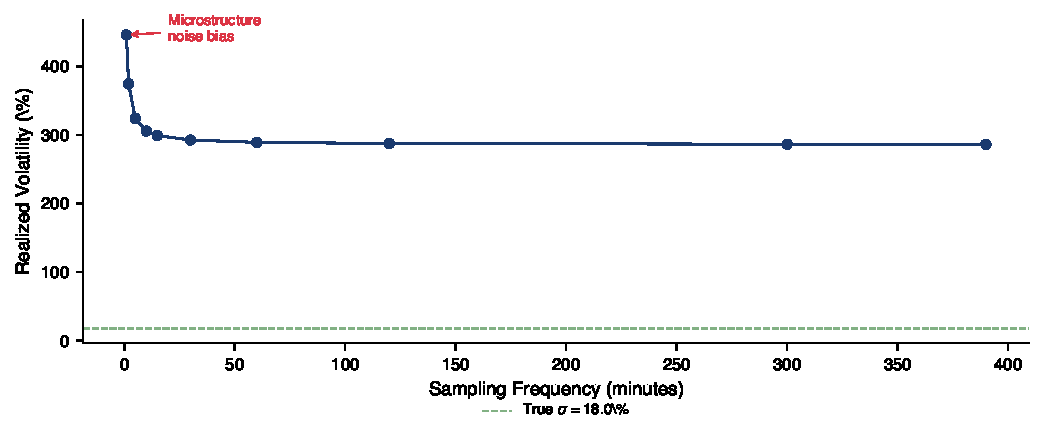
\includegraphics[width=0.80\linewidth]{sfm_ch1_vol_signature.pdf}
\end{center}
\vspace{-0.2cm}
\begin{itemize}\small\setlength{\itemsep}{0pt}
    \item La frecvențe înalte ($\Delta < 5$ min), bid-ask bounce umflă RV.
    \item La frecvențe joase, RV este nedeplasată dar imprecisă (puține observații).
    \item Eșantionare optimală: $\approx 5$ min echilibrează biasul și varianța (Bandi \& Russell, 2008).
\end{itemize}
\quantlet{SFM\_ch1\_vol\_comparison}{https://github.com/QuantLet/Stat_fin_markets/tree/master/Ch_01/SFM_ch1_vol_comparison}
\end{frame}

\begin{frame}{Estimatori de volatilitate: Graficul comparației de eficiență}
\begin{itemize}
    \item \textbf{RE} (Eficiență relativă) $= \Var(\hat{\sigma}^2_{\text{CC}}) / \Var(\hat{\sigma}^2)$.
    \item RE $> 1$: varianță mai mică decât benchmark-ul CC.
    \item Utilizarea OHLC vs.\ doar $C$: până la $14\times$ mai multă informație.
    \item YZ este cel mai bun estimator utilizând doar date OHLC zilnice.
    \item Intrazilic (RV): eficiență teoretic nelimitată când $\Delta \to 0$ (dacă microstructura permite).
\end{itemize}
\vspace{-0.15cm}
\begin{center}
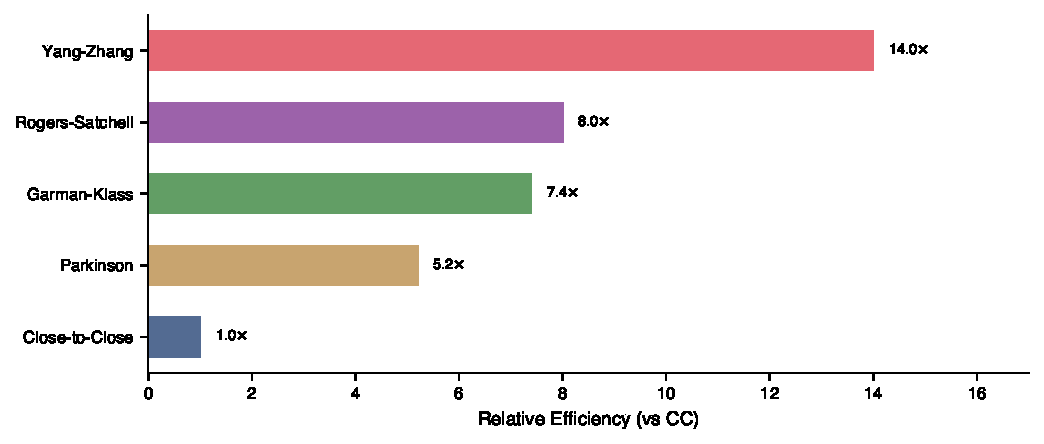
\includegraphics[width=0.55\linewidth]{sfm_ch1_efficiency.pdf}
\end{center}
\quantlet{SFM\_ch1\_volatility\_charts}{https://github.com/QuantLet/Stat_fin_markets/tree/master/Ch_01/SFM_ch1_volatility_charts}
\end{frame}

\begin{frame}{Volatilitate condițională vs.\ necondițională}
\begin{columns}[T]
\begin{column}{0.48\textwidth}
\begin{block}{Volatilitate necondițională}
\begin{itemize}
    \item Volatilitatea medie pe termen lung:
    \[
    \sigma^2 = \Var(r_t).
    \]
    \item Estimată prin estimatorul CC istoric pe o fereastră lungă.
    \item Constantă în timp: presupune staționaritate.
    \item Utilă pentru: evaluarea opțiunilor (termen lung), capital regulatoriu (Basel).
\end{itemize}
\end{block}
\end{column}
\begin{column}{0.48\textwidth}
\begin{block}{Volatilitate condițională}
\begin{itemize}
    \item Variabilă în timp, dată informația până la $t-1$:
    \[
    \sigma_t^2 = \Var(r_t \,|\, \mathcal{F}_{t-1}).
    \]
    \item Modelată prin ARCH/GARCH, volatilitate stochastică.
    \item Captează gruparea volatilității.
    \item Utilă pentru: riscul pe termen scurt, hedging opțiuni (delta), VaR.
\end{itemize}
\end{block}
\end{column}
\end{columns}
\vspace{0.15cm}
\begin{itemize}
    \item \textbf{GARCH(1,1)} (Bollerslev 1986): $\sigma_t^2 = \omega + \alpha r_{t-1}^2 + \beta\sigma_{t-1}^2$. Varianța pe termen lung (necondițională): $\bar{\sigma}^2 = \omega/(1-\alpha-\beta)$.
    \item Capitolul 5 acoperă modelele GARCH în detaliu.
\end{itemize}
\end{frame}

\begin{frame}{De ce volatilitatea nu este risc complet}
\begin{columns}[T]
\begin{column}{0.46\textwidth}
{\footnotesize
\textbf{Ce captează volatilitatea:}
\begin{itemize}\setlength{\itemsep}{0pt}
    \item Variabilitatea medie a randamentelor
    \item Dimensiunea fluctuațiilor tipice
    \item Baza pentru Sharpe ratio și VaR parametric
\end{itemize}
\vspace{0.1cm}
\textbf{\textcolor{Crimson}{Ce NU captează:}}
\begin{itemize}\setlength{\itemsep}{0pt}
    \item \textbf{Crash risk}: pierderi catastrofale
    \item \textbf{Tail risk}: evenimente extreme ($>3\sigma$)
    \item \textbf{Skewness}: asimetria distribuției
    \item \textbf{Drawdown}: cât poți pierde de la maxim
\end{itemize}
}
\end{column}
\begin{column}{0.50\textwidth}
{\footnotesize
\textbf{Exemplu ilustrativ:} Două active cu $\sigma = 20\%$:
\begin{itemize}\setlength{\itemsep}{0pt}
    \item \textbf{X}: Skewness $= 0$, $K = 3$ (Normală) --- mișcări $>3\sigma$: 1/370 zile
    \item \textbf{Y}: Skewness $= -1.5$, $K = 10$ --- mișcări $>3\sigma$: 1/50 zile
    \item Aceeași $\sigma$, \textbf{risc real complet diferit!}
\end{itemize}
}
\vspace{0.1cm}
\begin{block}{Concluzie}
\begin{itemize}
\item {\small Volatilitatea este \textit{necesară dar insuficientă}. Completați cu skewness, kurtosis, MDD și VaR/CVaR.}
\end{itemize}
\end{block}
\end{column}
\end{columns}
\end{frame}

\begin{frame}{Volatilitate condițională vs.\ necondițională: Exemplu AAPL}
\begin{center}
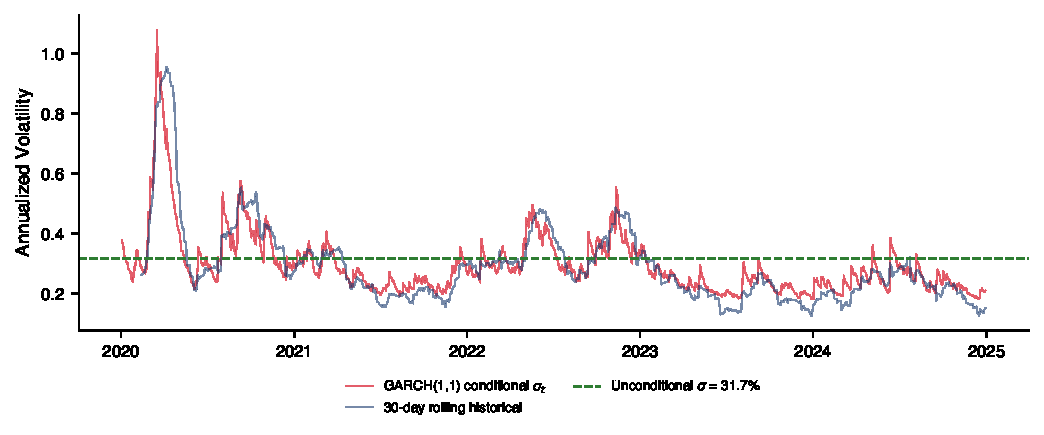
\includegraphics[width=0.82\linewidth]{sfm_ch1_cond_uncond.pdf}
\end{center}
\vspace{-0.2cm}
\begin{itemize}\small\setlength{\itemsep}{1pt}
    \item \textbf{GARCH(1,1)} urmărește gruparea volatilității în timp real.
    \item Estimarea rolling pe 30 de zile este mai netedă dar rămâne în urmă față de schimbările bruște.
    \item Nivelul necondițional = media pe termen lung în jurul căreia $\sigma_t$ fluctuează.
\end{itemize}
\quantlet{SFM\_ch1\_vol\_comparison}{https://github.com/QuantLet/Stat_fin_markets/tree/master/Ch_01/SFM_ch1_vol_comparison}
\end{frame}

%=============================================================================
% ACTUALIZARE CUPRINS după Secțiunea 5
%=============================================================================
{
\setbeamertemplate{headline}{%
    \vskip10pt%
    \hbox to \paperwidth{\hskip0.5cm\hfill\hskip0.5cm}%
    \vskip4pt%
    {\color{FooterGray}\hrule height 0.4pt}%
}
\begin{frame}{}
    {\color{FooterGray}\hrule height 0.4pt}
    \vspace{0.1cm}
    {\Large\textcolor{IDAred}{\textbf{Cuprins}}}
    \vspace{0.2cm}
    \begin{enumerate}
        \item Motivație \checkmark
        \item Date de preț \checkmark
        \item Randamente \checkmark
        \item Fapte stilizate ale randamentelor financiare \checkmark
        \item Estimatori de volatilitate \checkmark
        \item \textbf{Comparație de eficiență}
        \item Randamente ajustate la risc
        \item Caz AI / Rezumat / Quiz
        \item Bibliografie
    \end{enumerate}
\end{frame}
}

%=============================================================================
% SECȚIUNEA 6: COMPARAȚIE DE EFICIENȚĂ
%=============================================================================
\section{Comparație de eficiență}

\begin{frame}{Eficiența estimatorilor de volatilitate}
\begin{itemize}
    \item \textbf{Eficiență relativă}: $\text{RE} = \Var(\hat{\sigma}^2_{\text{CC}}) / \Var(\hat{\sigma}^2)$.\quad RE $> 1$ înseamnă varianță mai mică decât CC.
    \item \textbf{Interpretare intuitivă}: \textit{„Dacă RE $= 5$, înseamnă că avem nevoie de $5\times$ mai puține date pentru aceeași precizie."} Sau echivalent: cu aceeași cantitate de date, estimarea este de $5\times$ mai precisă.
\end{itemize}
\vspace{0.1cm}
\begin{center}
{\small
\renewcommand{\arraystretch}{1.25}
\begin{tabular}{lcccl}
\toprule
\textbf{Estimator} & \textbf{RE vs.\ CC} & \textbf{Ind.\ de drift?} & \textbf{Robust salturi?} & \textbf{Date} \\
\midrule
Close-to-Close & 1.0 & Nu & Nu & $C$ \\
Parkinson & 5.2 & Da ($\mu=0$) & Nu & $H,L$ \\
Garman-Klass & 7.4 & Da ($\mu=0$) & Nu & $O,H,L,C$ \\
Rogers-Satchell & 8.0 & \textcolor{Forest}{Permite drift} & Nu & $O,H,L,C$ \\
Yang-Zhang & 14.0 & \textcolor{Forest}{Permite drift} & Parțial & $O,H,L,C$ \\
Realized Vol & $\gg$14 & Da & Extensii & Intrazilnice \\
\bottomrule
\end{tabular}
}
\end{center}
\vspace{0.1cm}
\begin{itemize}
    \item Toți estimatorii bazați pe interval presupun \textbf{tranzacționare continuă} și \textbf{fără salturi de preț}.
    \item În practică, sunt disponibile extensii robuste la salturi (bipower variation, Christensen \& Podolskij 2007).
    \item Gap-urile overnight încalcă ipoteza de tranzacționare continuă pentru GK, Parkinson.
\end{itemize}
\end{frame}

\begin{frame}{Considerații practice}
\begin{columns}[T]
\begin{column}{0.50\textwidth}
\begin{block}{Când folosim care?}
\begin{itemize}
    \item \textbf{CC}: doar prețuri de închidere disponibile.
    \item \textbf{Parkinson}: estimare rapidă de interval; piețe fără drift.
    \item \textbf{GK}: cea mai bună eficiență când drift $\approx 0$.
    \item \textbf{RS}: piețe în trend, drift semnificativ.
    \item \textbf{YZ}: cel mai bun estimator general pentru OHLC zilnic.
    \item \textbf{RV}: date intra-zilnice; standardul de aur.
\end{itemize}
\end{block}
\end{column}
\begin{column}{0.46\textwidth}
\begin{block}{Capcane frecvente}
\begin{itemize}
    \item GK/Parkinson pe date în trend $\Rightarrow$ distorsionat în jos.
    \item Ignorarea gap-urilor overnight $\Rightarrow$ subestimează vol totală.
    \item Fereastră prea scurtă $\Rightarrow$ zgomotoasă; prea lungă $\Rightarrow$ depășită.
    \item Prețuri neajustate $\Rightarrow$ salturi false la datele dividendelor.
\end{itemize}
\end{block}
\begin{alertblock}{Regulă practică}
\begin{itemize}\setlength{\itemsep}{0pt}
    \item 20--30z: termen scurt; 60--90z: termen mediu; 252z: anual.
\end{itemize}
\end{alertblock}
\end{column}
\end{columns}
\end{frame}

%=============================================================================
% ACTUALIZARE CUPRINS după Secțiunea 6
%=============================================================================
{
\setbeamertemplate{headline}{%
    \vskip10pt%
    \hbox to \paperwidth{\hskip0.5cm\hfill\hskip0.5cm}%
    \vskip4pt%
    {\color{FooterGray}\hrule height 0.4pt}%
}
\begin{frame}{}
    {\color{FooterGray}\hrule height 0.4pt}
    \vspace{0.1cm}
    {\Large\textcolor{IDAred}{\textbf{Cuprins}}}
    \vspace{0.2cm}
    \begin{enumerate}
        \item Motivație \checkmark
        \item Date de preț \checkmark
        \item Randamente \checkmark
        \item Fapte stilizate ale randamentelor financiare \checkmark
        \item Estimatori de volatilitate \checkmark
        \item Comparație de eficiență \checkmark
        \item \textbf{Randamente ajustate la risc}
        \item Caz AI / Rezumat / Quiz
        \item Bibliografie
    \end{enumerate}
\end{frame}
}

%=============================================================================
% SECȚIUNEA 7: RANDAMENTE AJUSTATE LA RISC
%=============================================================================
\section{Randamente ajustate la risc}

\begin{frame}{Indicatorul Sharpe}
\begin{columns}[T]
\begin{column}{0.44\textwidth}
\begin{defn}[Indicatorul Sharpe]
\begin{itemize}\setlength{\itemsep}{1pt}
    \item Randament excesiv pe unitate de risc total:
    $SR = \frac{\bar{R}_p - R_f}{\sigma_p}.$
\end{itemize}
\end{defn}
\vspace{0.05cm}
\begin{itemize}\small\setlength{\itemsep}{1pt}
    \item S\&P 500: $SR\approx 0.4$--$0.5$ (anual).
    \item SR mai mare $\not\Rightarrow$ performanță viitoare superioară.
    \item Presupune normalitate; eșuează pentru randamente asimetrice.
\end{itemize}
\end{column}
\begin{column}{0.52\textwidth}
\begin{center}
{\small
\renewcommand{\arraystretch}{1.15}
\begin{tabular}{cl}
\toprule
\textbf{Valoare SR} & \textbf{Interpretare} \\
\midrule
$SR < 0$ & \textcolor{Crimson}{Sub rata fără risc} \\
$0 \leq SR < 1$ & \textcolor{Amber}{Acceptabil} \\
$1 \leq SR < 2$ & \textcolor{Forest}{Bun} \\
$SR \geq 2$ & \textcolor{MainBlue}{Excelent (rar)} \\
\bottomrule
\end{tabular}
}
\end{center}
\end{column}
\end{columns}
\quantlet{SFM\_ch1\_sharpe\_ratio}{https://github.com/QuantLet/Stat_fin_markets/tree/master/Ch_01/SFM_ch1_sharpe_ratio}
\end{frame}

\begin{frame}{Limitări ale indicatorului Sharpe}
\begin{alertblock}{Limitări}
\begin{itemize}\setlength{\itemsep}{2pt}
    \item \textbf{Penalizează și volatilitatea pozitivă} --- nu diferențiază câștiguri de pierderi
    \item \textbf{Nu capturează asimetria} (skew) --- pierderi rare dar catastrofale $\Rightarrow$ SR bun
    \item \textbf{Ignoră drawdown-ul} --- nu spune nimic despre cel mai rău scenariu
    \item \textbf{Nu capturează riscul de coadă} --- SR ridicat nu înseamnă lipsă de tail risk
    \item \textbf{Eroare de estimare mare} --- Lo (2002): $\text{SE}(\widehat{SR}) \approx \sqrt{(1 + SR^2/2)\,/\,n}$. Ex.: cu $SR=0.5$ și $n=60$ luni, $\text{SE}\approx 0.13$, deci intervalul de încredere 95\% este $[0.24,\;0.76]$ --- foarte larg!
\end{itemize}
\end{alertblock}
\end{frame}

\begin{frame}{Indicatorul Sharpe: Exemplu numeric}
\begin{example}
Două fonduri, $R_f = 2\%$ pe an. Care oferă un randament ajustat la risc mai bun?
\end{example}
\vspace{0.05cm}
\begin{center}
{\small
\renewcommand{\arraystretch}{1.2}
\begin{tabular}{lcccc}
\toprule
\textbf{Fond} & $\bar{R}_p$ & $\sigma_p$ & $\bar{R}_p - R_f$ & $SR$ \\
\midrule
Fond A & $12\%$ & $18\%$ & $10\%$ & $10/18 = \mathbf{0{,}556}$ \\
Fond B & $8\%$ & $9\%$ & $6\%$ & $6/9 = \mathbf{0{,}667}$ \\
\bottomrule
\end{tabular}
}
\end{center}
\vspace{0.05cm}
\begin{itemize}
    \item Fondul B: randament absolut mai mic dar indicator Sharpe mai mare.
    \item Investitorul avers la risc preferă Fondul B (recompensă mai bună per unitate de risc).
    \item Fondul A necesită $18\times0.667+2=14\%$ randament pentru a egala SR-ul Fondului B.
\end{itemize}
\begin{block}{Anualizarea SR}
\begin{itemize}
\item Din date zilnice: $SR_{\text{annual}} = SR_{\text{daily}} \times \sqrt{252}$.
\end{itemize}
\end{block}
\end{frame}

\begin{frame}{Alte măsuri ajustate la risc (I)}
\begin{itemize}
    \item \textbf{Sortino Ratio}: utilizează deviația descendentă $\sigma_D$ sub un prag $\tau$ (de obicei $R_f$ sau 0):
    \[
    \text{Sortino} = \frac{\bar{R}_p - \tau}{\sigma_D}, \qquad \sigma_D = \sqrt{\frac{1}{n}\sum_{t=1}^{n}\bigl[\min(R_t - \tau,\;0)\bigr]^2}.
    \]
    Preferat când distribuția randamentelor este asimetrică (opțiuni long, fonduri speculative).\\
    {\footnotesize\textit{Notă}: unii autori utilizează $1/n_-$ (doar observațiile negative) în loc de $1/n$ la numitor, ceea ce produce valori mai mari ale $\sigma_D$.}
    \item \textbf{Raportul informațional} (IR): randament activ vs. eroare de urmărire față de benchmark $B$:
    \[
    \text{IR} = \frac{\bar{R}_p - \bar{R}_B}{\text{TE}}, \qquad \text{TE} = \text{std}(R_p - R_B).
    \]
    \item \textbf{Calmar Ratio}: randament raportat la drawdown-ul maxim:
    \[
    \text{Calmar} = \frac{\bar{R}_{\text{annual}}}{|\text{MDD}|}.
    \]
\end{itemize}
\end{frame}

\begin{frame}{Alte măsuri ajustate la risc (II)}
\begin{itemize}
    \item \textbf{Treynor Ratio}: randament excesiv pe unitate de risc \textit{sistematic}:
    \[
    \text{Treynor} = \frac{\bar{R}_p - R_f}{\beta_p}, \qquad \beta_p = \Cov(R_p, R_m)/\Var(R_m).
    \]
    \item \textbf{Omega Ratio} (Keating \& Shadwick, 2002): raportul câștigurilor ponderate deasupra pragului $\tau$ la pierderile de sub $\tau$:
    \[
    \Omega(\tau) = \frac{\int_{\tau}^{\infty}[1 - F(r)]\,dr}{\int_{-\infty}^{\tau}F(r)\,dr}, \qquad F = \text{CDF a randamentelor}.
    \]
    Interpretare: $\Omega > 1$ distribuție favorabilă; $\Omega < 1$ nefavorabilă. Captează \textit{întreaga} distribuție, nu doar primele momente.
\end{itemize}
\end{frame}

\begin{frame}{Volatilitatea portofoliului}
\begin{itemize}
    \item Pentru un portofoliu cu două active cu ponderile $w_X + w_Y = 1$:
    \[
    \sigma_P^2 = w_X^2\sigma_X^2 + w_Y^2\sigma_Y^2 + 2w_X w_Y\,\rho_{XY}\,\sigma_X\sigma_Y.
    \]
    \item \textbf{Beneficiul diversificării}: când $\rho_{XY} < 1$, varianța portofoliului $< $ varianța medie ponderată.
    \item Beneficiu maxim când $\rho_{XY} = -1$ (corelație negativă perfectă).
\end{itemize}
\vspace{0.1cm}
\begin{example}
$w_X = 0.6$, $w_Y = 0.4$; $\sigma_X = 20\%$, $\sigma_Y = 30\%$; $\rho = 0.3$.
\[
\sigma_P^2 = (0.6)^2(0.20)^2 + (0.4)^2(0.30)^2 + 2(0.6)(0.4)(0.3)(0.20)(0.30)
\]
\[
= 0.0144 + 0.0144 + 0.00864 = 0.03744. \quad \sigma_P = 19.35\%.
\]
Medie ponderată: $0.6 \times 20\% + 0.4 \times 30\% = 24\%$.
Diversificarea economisește $\approx 4.65\%$ din volatilitate.
\end{example}
\end{frame}

\begin{frame}{Exemplu: Portofoliu cu 3 active}
\begin{example}
Trei active cu $\sigma_1 = 20\%$, $\sigma_2 = 25\%$, $\sigma_3 = 15\%$ și matricea de corelație:
\[
\boldsymbol{\rho} = \begin{pmatrix} 1 & 0.3 & 0.1 \\ 0.3 & 1 & 0.25 \\ 0.1 & 0.25 & 1 \end{pmatrix}, \qquad \mathbf{w} = \left(\tfrac{1}{3},\;\tfrac{1}{3},\;\tfrac{1}{3}\right).
\]
\end{example}
\vspace{0.1cm}
\begin{itemize}\small\setlength{\itemsep}{1pt}
    \item Formula generală: $\sigma_P^2 = \mathbf{w}'\boldsymbol{\Sigma}\mathbf{w} = \sum_{i}\sum_{j} w_i w_j \rho_{ij}\sigma_i\sigma_j$.
    \item Calculul:
    {\footnotesize
    \begin{align*}
    \sigma_P^2 &= \tfrac{1}{9}\bigl[\sigma_1^2 + \sigma_2^2 + \sigma_3^2 + 2\rho_{12}\sigma_1\sigma_2 + 2\rho_{13}\sigma_1\sigma_3 + 2\rho_{23}\sigma_2\sigma_3\bigr] \\
    &= \tfrac{1}{9}\bigl[0.04 + 0.0625 + 0.0225 + 2(0.3)(0.05) + 2(0.1)(0.03) + 2(0.25)(0.0375)\bigr] \\
    &= \tfrac{1}{9}\bigl[0.125 + 0.03 + 0.006 + 0.01875\bigr] = \tfrac{0.17975}{9} = 0.01997.
    \end{align*}}
    \item $\sigma_P = \sqrt{0.01997} = 14.13\%$.
    \item Media ponderată: $\tfrac{1}{3}(20\% + 25\% + 15\%) = 20\%$.
    \item \textbf{Beneficiul diversificării}: $20\% - 14.13\% \approx 5.87\%$ economie de volatilitate.
\end{itemize}
\end{frame}

\begin{frame}[shrink=3]{Frontiera eficientă}
\begin{itemize}
    \item \textbf{Frontiera eficientă} (\textit{efficient frontier}): mulțimea portofoliilor cu randament așteptat maxim pentru o volatilitate dată (Markowitz 1952).
    \item \textbf{MVP}: portofoliul cu varianță minimă --- cel mai mic $\sigma_P$.
    \item \textbf{Portofoliul tangent} (\textit{tangency portfolio}): portofoliul de pe frontieră cu cel mai mare indicator Sharpe.
    \item \textbf{Linia pieței de capital} (CML): combinații de $R_f$ și portofoliul tangent.
    \item Toți investitorii raționali dețin o combinație de $R_f$ și portofoliul tangent (Teorema separației, Tobin 1958).
\end{itemize}
\vspace{-0.15cm}
\begin{center}
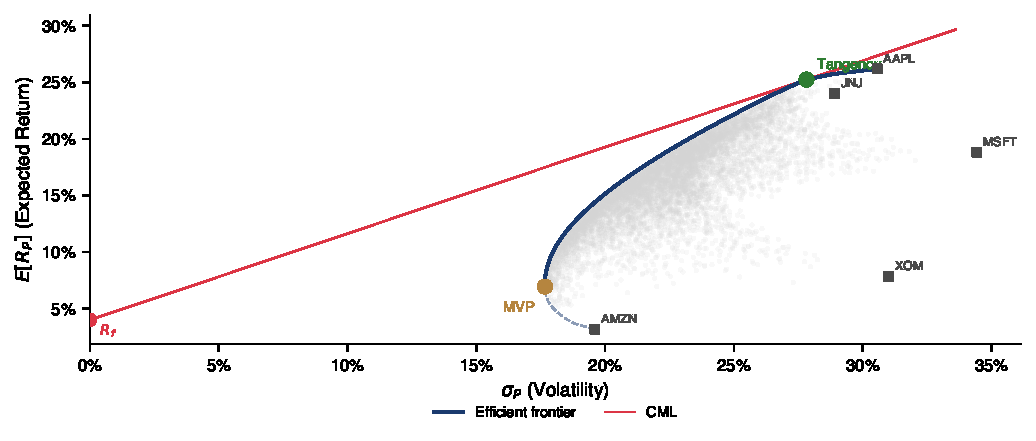
\includegraphics[width=0.55\linewidth]{sfm_ch1_frontier.pdf}
\end{center}
\quantlet{SFM\_ch1\_volatility\_charts}{https://github.com/QuantLet/Stat_fin_markets/tree/master/Ch_01/SFM_ch1_volatility_charts}
\end{frame}

\begin{frame}{Markowitz vs.\ Linia Pieței de Capital}
\begin{columns}[T]
\begin{column}{0.48\textwidth}
\begin{block}{Fără activ fără risc (Markowitz)}
\begin{itemize}\setlength{\itemsep}{1pt}
    \item Mulțimea fezabilă: \textbf{curba tip glonț} (\textit{bullet curve}) în planul $(\sigma, \E[R])$
    \item Frontiera eficientă: porțiunea superioară a curbei, deasupra MVP
    \item Fiecare investitor alege un portofoliu \textbf{diferit} pe frontieră, în funcție de aversiunea la risc
    \item Nu există un portofoliu \textit{universal} optim
\end{itemize}
\end{block}
\end{column}
\begin{column}{0.48\textwidth}
\begin{exampleblock}{Cu activ fără risc (Tobin)}
\begin{itemize}\setlength{\itemsep}{1pt}
    \item CML: linie dreaptă de la $R_f$ tangentă la frontieră
    \item Portofoliul tangent $T$ este \textbf{unic} și optim pentru toți investitorii
    \item Teorema separării în două fonduri: orice portofoliu eficient $= $ combinație de $R_f$ și $T$
    \item Aversiunea la risc determină doar \textbf{ponderea} în $T$, nu compoziția
\end{itemize}
\end{exampleblock}
\end{column}
\end{columns}
\vspace{0.2cm}
\begin{alertblock}{Concluzie}
\begin{itemize}
\item \small Introducerea activului fără risc \textbf{simplifică radical} alegerea: de la o curbă (infinitate de portofolii eficiente) la un singur punct (portofoliul tangent) plus o decizie de levier.
\end{itemize}
\end{alertblock}
\end{frame}

\begin{frame}{Portofoliul cu varianță minimă (MVP)}
\begin{itemize}
    \item \textbf{Problema de optimizare medie-varianță} (Markowitz, 1952):
\end{itemize}
\[
\min_{\mathbf{w}} \;\; \mathbf{w}'\boldsymbol{\Sigma}\mathbf{w} \qquad \text{s.t.} \quad \mathbf{w}'\boldsymbol{\mu} = \mu_{\text{target}}, \quad \mathbf{w}'\mathbf{1} = 1.
\]
\begin{itemize}
    \item \textbf{MVP global} (fără constrângere de randament țintă):
    \[
    \mathbf{w}_{\text{MVP}} = \frac{\boldsymbol{\Sigma}^{-1}\mathbf{1}}{\mathbf{1}'\boldsymbol{\Sigma}^{-1}\mathbf{1}}, \qquad \sigma_{\text{MVP}}^2 = \frac{1}{\mathbf{1}'\boldsymbol{\Sigma}^{-1}\mathbf{1}}.
    \]
    \item MVP depinde \textit{doar} de matricea de covarianță $\boldsymbol{\Sigma}$, nu de randamentele așteptate $\boldsymbol{\mu}$.
    \item Acest lucru îl face mai robust în practică, deoarece $\boldsymbol{\mu}$ este notoriu greu de estimat (Merton, 1980).
    \item Frontiera eficientă este ramura superioară a ``glonțului'' trasată variind $\mu_{\text{target}}$ de la $\mu_{\text{MVP}}$ la $\max(\boldsymbol{\mu})$.
\end{itemize}
\end{frame}

\begin{frame}{Teorema separării cu două fonduri (Two-Fund Separation)}
\begin{thm}[Tobin, 1958]
Orice portofoliu eficient poate fi exprimat ca o combinație liniară a doar două portofolii de pe frontiera eficientă.
\end{thm}
\vspace{0.1cm}
\begin{itemize}
    \item \textbf{Fără activ fără risc}: fiecare investitor alege pe frontieră în funcție de toleranța sa la risc. Toate alegerile eficiente sunt amestecuri ale acelorași două ``fonduri mutuale.''
    \item \textbf{Cu activ fără risc} $R_f$: frontiera se reduce la \textbf{Capital Market Line} (CML):
    \[
    E[R_P] = R_f + \frac{E[R_T] - R_f}{\sigma_T}\,\sigma_P,
    \]
    unde $T$ = \textbf{portofoliul tangent} (cel cu Sharpe maxim).
    \item \textbf{Consecință}: toți investitorii dețin \textit{același} portofoliu riscant $T$; diferă doar proporția investită în $R_f$ (levier sau de-levier).
    \item \textbf{Implicație practică}: portofoliul de piață $\approx T$ $\Rightarrow$ baza teoretică a \textbf{investiției pasive în indici}.
\end{itemize}
\end{frame}

%=============================================================================
% ACTUALIZARE CUPRINS după Secțiunea 7
%=============================================================================
{
\setbeamertemplate{headline}{%
    \vskip10pt%
    \hbox to \paperwidth{\hskip0.5cm\hfill\hskip0.5cm}%
    \vskip4pt%
    {\color{FooterGray}\hrule height 0.4pt}%
}
\begin{frame}{}
    {\color{FooterGray}\hrule height 0.4pt}
    \vspace{0.1cm}
    {\Large\textcolor{IDAred}{\textbf{Cuprins}}}
    \vspace{0.2cm}
    \begin{enumerate}
        \item Motivație \checkmark
        \item Date de preț \checkmark
        \item Randamente \checkmark
        \item Fapte stilizate ale randamentelor financiare \checkmark
        \item Estimatori de volatilitate \checkmark
        \item Comparație de eficiență \checkmark
        \item Randamente ajustate la risc \checkmark
        \item \textbf{Caz de utilizare AI}
        \item Rezumat
        \item Quiz
        \item Bibliografie
    \end{enumerate}
\end{frame}
}

%=============================================================================
% SECȚIUNEA 8: CAZ DE UTILIZARE AI
%=============================================================================
\section{Caz de utilizare AI}

\begin{frame}[shrink=3]{Exercițiu AI: Gândire critică}
    \begin{cminipage}{0.95\textwidth}
    \begin{block}{\footnotesize Prompt de testat în ChatGPT / Claude / Copilot}
        {\small
        ``Descarcă datele zilnice OHLC pentru AAPL 2020--2024 folosind Python (\texttt{yfinance}).
        Calculează toți cei cinci estimatori de volatilitate (CC, Parkinson, Garman-Klass, Rogers-Satchell, Yang-Zhang)
        folosind o fereastră rolling de 30 de zile. Reprezintă-i pe același grafic și calculează estimările anualizate pe întregul eșantion.
        De asemenea, estimează un model GARCH(1,1) și suprapune volatilitatea condițională. Discută care estimator este cel mai fiabil.''
        }
    \end{block}
    \vspace{-1mm}
    {\small
    \textbf{Exercițiu}:
    \begin{enumerate}
        \item AI-ul folosește formula corectă pentru fiecare estimator? Verifică cu notele de curs.
        \item Sunt clasamentele de eficiență (rapoartele RE) consistente cu teoria?
        \item Volatilitatea condițională GARCH urmărește gruparea volatilității mai bine decât estimările rolling?
        \item Întreabă AI-ul: ``Ce se întâmplă dacă acțiunea are gap-uri overnight?'' Menționează Yang-Zhang?
        \item Re-rulează cu date BTC-USD. Se schimbă clasamentul estimatorilor? De ce?
    \end{enumerate}
    }
    \vspace{-1mm}
    \begin{alertblock}{}
        {\small
        \begin{itemize}\setlength{\itemsep}{0pt}
            \item \textbf{Atenție}: AI-ul confundă adesea formula Rogers-Satchell. Verificați mereu cu $\ln(H/C)\cdot\ln(H/O) + \ln(L/C)\cdot\ln(L/O)$.
        \end{itemize}
        }
    \end{alertblock}
    \end{cminipage}
\end{frame}

%=============================================================================
% ACTUALIZARE CUPRINS după Caz AI
%=============================================================================
{
\setbeamertemplate{headline}{%
    \vskip10pt%
    \hbox to \paperwidth{\hskip0.5cm\hfill\hskip0.5cm}%
    \vskip4pt%
    {\color{FooterGray}\hrule height 0.4pt}%
}
\begin{frame}{}
    {\color{FooterGray}\hrule height 0.4pt}
    \vspace{0.1cm}
    {\Large\textcolor{IDAred}{\textbf{Cuprins}}}
    \vspace{0.2cm}
    {\small
    \begin{columns}[T]
        \begin{column}{0.48\textwidth}
            \begin{enumerate}
                \item Motivație \checkmark
                \item Date de preț \checkmark
                \item Randamente \checkmark
                \item Fapte stilizate \checkmark
                \item Estimatori de volatilitate \checkmark
                \item Comparație de eficiență \checkmark
            \end{enumerate}
        \end{column}
        \begin{column}{0.48\textwidth}
            \begin{enumerate}\setcounter{enumi}{6}
                \item Randamente ajustate la risc \checkmark
                \item Caz de utilizare AI \checkmark
                \item \textbf{Rezumat}
                \item Quiz
                \item Bibliografie
            \end{enumerate}
        \end{column}
    \end{columns}
    }
\end{frame}
}

%=============================================================================
% SECȚIUNEA 9: REZUMAT
%=============================================================================
\section{Rezumat}

\begin{frame}{Concluzii cheie}
    \begin{block}{Rezumat}
    \small
    \begin{itemize}
        \item \textbf{Randamentele} sunt metrica principală:
        \begin{itemize}
            \item Randamente simple pentru analiză cross-secțională; randamente logaritmice pentru serii de timp
            \item Pierderea din varianță: $\E[r] \approx \E[R] - \sigma^2/2$; critică pentru active volatile
        \end{itemize}
        \item \textbf{Fapte stilizate} universale: cozi groase, gruparea volatilității, efect levier, normalitate prin agregare
        \item \textbf{Volatilitatea} este o variabilă latentă; estimatorii bazați pe range (P, GK, RS, YZ) sunt mai eficienți decât CC
        \item \textbf{Măsuri ajustate la risc}: Sharpe ratio este standard; Sortino, Calmar abordează limitările
        \item \textbf{Diversificare}: frontiera eficientă formalizează compromisul risc-randament (Markowitz 1952)
    \end{itemize}
    \end{block}
\end{frame}

\begin{frame}{Formule importante}
    \begin{columns}[T]
        \begin{column}{0.48\textwidth}
        {\small
        \begin{block}{Randamente}
            \begin{itemize}
                \item \textbf{Simple}: $R_t = P_t/P_{t-1} - 1$
                \item \textbf{Log}: $r_t = \ln(P_t/P_{t-1})$
                \item \textbf{Pierdere}: $\E[r] \approx \E[R] - \sigma^2/2$
                \item \textbf{Scalare}: $\sigma_T = \sigma_1\sqrt{T}$
            \end{itemize}
        \end{block}
        \begin{alertblock}{Estimatori de volatilitate}
            \begin{itemize}
                \item \textbf{CC}: $\hat\sigma^2 = \frac{1}{n-1}\sum (r_t - \bar{r})^2$
                \item \textbf{Parkinson}: folosește $\ln(H/L)$
                \item \textbf{YZ}: combină overnight + RS
            \end{itemize}
        \end{alertblock}
        }
        \end{column}
        \begin{column}{0.48\textwidth}
        {\small
        \begin{exampleblock}{Randamente ajustate la risc}
            \begin{itemize}
                \item \textbf{Sharpe}: $SR = (\bar{R} - R_f)/\sigma$
                \item \textbf{Sortino}: folosește $\sigma_D$ descendentă
                \item \textbf{Portofoliu}: $\sigma_P^2 = \mathbf{w}'\Sigma\mathbf{w}$
            \end{itemize}
        \end{exampleblock}
        \begin{block}{GARCH(1,1)}
            \begin{itemize}
                \item $\sigma_t^2 = \omega + \alpha r_{t-1}^2 + \beta\sigma_{t-1}^2$
                \item \textbf{Necond.}: $\bar\sigma^2 = \frac{\omega}{1-\alpha-\beta}$
                \item \textbf{EWMA}: $\lambda = 0{,}94$
            \end{itemize}
        \end{block}
        }
        \end{column}
    \end{columns}
\end{frame}

\begin{frame}[shrink=3]{Capcane frecvente}
\begin{columns}[T]
\begin{column}{0.48\textwidth}
\begin{alertblock}{Erori de date}
\begin{itemize}\setlength{\itemsep}{1pt}
    \item Folosirea \textbf{prețurilor neajustate} la dividende/splituri
    \item Ignorarea \textbf{survivorship bias} (doar firme active)
    \item Confuzia între preț și randament
\end{itemize}
\end{alertblock}
\vspace{0.05cm}
\begin{alertblock}{Erori de calcul}
\begin{itemize}\setlength{\itemsep}{1pt}
    \item \textbf{Anualizare greșită}: $\sigma_{\text{annual}} = \sigma_{\text{daily}} \times 252$ în loc de $\times\sqrt{252}$
    \item Aplicarea regulii $\sqrt{T}$ \textbf{fără verificarea i.i.d.}
    \item Adunarea randamentelor simple pe timp (sunt multiplicative!)
\end{itemize}
\end{alertblock}
\end{column}
\begin{column}{0.48\textwidth}
\begin{alertblock}{Erori de interpretare}
\begin{itemize}\setlength{\itemsep}{1pt}
    \item Interpretarea Sharpe \textbf{fără risc sistemic}: SR mare $\neq$ risc mic
    \item Ignorarea \textbf{asimetriei/curtozei}: SR nu captează riscul de coadă
    \item Presupunerea de \textbf{normalitate} la VaR: subestimează pierderile extreme
    \item Confuzia dintre \textbf{corelație și cauzalitate}
\end{itemize}
\end{alertblock}
\vspace{0.05cm}
\begin{alertblock}{Erori de estimare}
\begin{itemize}\setlength{\itemsep}{1pt}
    \item Fereastră prea \textbf{scurtă} $\Rightarrow$ zgomot; prea \textbf{lungă} $\Rightarrow$ depășită
    \item GK/Parkinson pe piețe \textbf{în trend} $\Rightarrow$ distorsionat
    \item Ignorarea \textbf{gap-urilor overnight}
\end{itemize}
\end{alertblock}
\end{column}
\end{columns}
\end{frame}

\begin{frame}[shrink=5]{Ce trebuie să știți perfect}
\begin{block}{Checklist de competențe --- Capitolul 1}
\begin{columns}[T]
\begin{column}{0.48\textwidth}
\begin{enumerate}
    \item[\checkmark] \textbf{Calculați} randamente simple și logaritmice din prețuri
    \item[\checkmark] \textbf{Explicați} diferența simplă vs.\ log și când se folosește fiecare
    \item[\checkmark] \textbf{Calculați} și interpretați pierderea din varianță (variance drag)
    \item[\checkmark] \textbf{Anualizați} corect volatilitatea ($\times\sqrt{252}$, nu $\times 252$)
    \item[\checkmark] \textbf{Aplicați} regula $\sqrt{T}$ și cunoașteți limitările ei
    \item[\checkmark] \textbf{Distingeți} între estimatorii CC, Parkinson, GK, RS, Yang-Zhang
\end{enumerate}
\end{column}
\begin{column}{0.48\textwidth}
\begin{enumerate}\setcounter{enumi}{6}
    \item[\checkmark] \textbf{Interpretați} asimetria: $S < 0$ $\Rightarrow$ pierderi mari mai frecvente
    \item[\checkmark] \textbf{Interpretați} kurtosis: $K > 3$ $\Rightarrow$ cozi groase, normala inadecvată
    \item[\checkmark] \textbf{Calculați} indicatorul Sharpe și cunoașteți limitările
    \item[\checkmark] \textbf{Calculați} drawdown și MDD
    \item[\checkmark] \textbf{Explicați} faptele stilizate: gruparea volatilității, efect levier, cozi groase
    \item[\checkmark] \textbf{Distingeți} volatilitate istorică, condițională, realizată, implicită
\end{enumerate}
\end{column}
\end{columns}
\end{block}
\vspace{0.1cm}
\begin{exampleblock}{Test rapid de autoevaluare}
\begin{itemize}\setlength{\itemsep}{0pt}
    \item Dacă puteți răspunde la toate cele 12 puncte \textbf{fără note}, sunteți pregătiți pentru examen pe acest capitol.
\end{itemize}
\end{exampleblock}
\end{frame}

\begin{frame}{Previzualizare capitolul următor}
    \begin{columns}[T]
        \begin{column}{0.48\textwidth}
        \begin{block}{Capitolul 2: Distribuții de probabilitate pentru piețele financiare}
            \begin{itemize}
                \item \textbf{Distribuția Normală}: proprietăți, limitări pentru date financiare
                \item \textbf{Student-$t$}: cozi groase, grade de libertate
                \item \textbf{Distribuții stabile}: Pareto-stabile, legi de putere
                \item \textbf{Amestecuri}: Normal Inverse Gaussian (NIG), modele de amestec
            \end{itemize}
        \end{block}
        \end{column}
        \begin{column}{0.48\textwidth}
        \begin{exampleblock}{Ce vom învăța}
            \begin{itemize}
                \item \textbf{Comparați} distribuții pe date reale (QQ-plot, testul KS)
                \item \textbf{Estimați} parametrii prin MLE
                \item \textbf{Modelați} cozile groase și asimetria
                \item \textbf{Aplicați} distribuții în context financiar
            \end{itemize}
        \end{exampleblock}
        \end{column}
    \end{columns}
\end{frame}

%=============================================================================
% TEME
%=============================================================================

\begin{frame}{Tema 1: Calculul randamentelor}
\begin{itemize}
    \item Prețul unei acțiuni la momentul $t$ este $P_t = \$100$.
    \begin{itemize}
        \item Randamentele compuse continuu (log) pe următoarele trei perioade sunt:
        $r_{t+1} = 0.10$,\; $r_{t+2} = -0.05$,\; $r_{t+3} = 0.02$.
        \item Calculați $P_{t+1}$, $P_{t+2}$, $P_{t+3}$. Arătați toate calculele.
    \end{itemize}
    \item Acum presupuneți că randamentele \textbf{simple} sunt $R_{t+1} = 0.10$, $R_{t+2} = -0.05$, $R_{t+3} = 0.02$.
    \begin{itemize}
        \item Calculați $P_{t+1}$, $P_{t+2}$, $P_{t+3}$. Arătați toate calculele.
    \end{itemize}
    \item Comparați prețurile finale:
    \begin{itemize}
        \item Sunt identice? De ce da sau de ce nu?
        \item Care este mai mare și cu cât?
        \item Explicați implicațiile practice, în special pentru orizonturi mai lungi.
    \end{itemize}
\end{itemize}
\end{frame}

\begin{frame}{Tema 1 (cont.): Aditivitatea temporală}
\begin{itemize}
    \item Vi se dă o serie temporală de prețuri ale acțiunilor $P_0, P_1, \ldots, P_n$.
    \begin{itemize}
        \item Derivați o formulă generală pentru randamentul total compus continuu de la momentul $0$ la momentul $n$.
        \item Exprimați aceasta în funcție de randamentele logaritmice individuale pe perioadă $r_1, r_2, \ldots, r_n$.
        \item Explicați cum se aplică \textbf{aditivitatea temporală} la randamentele logaritmice.
        \item De ce este această proprietate dezirabilă în modelarea financiară (ex., pentru scalarea varianței)?
    \end{itemize}
    \item Derivați acum formula analogă pentru \textbf{randamentul simplu} total pe $n$ perioade.
    \begin{itemize}
        \item Arătați că randamentele simple \textbf{nu} sunt aditive temporal.
        \item Oferiți un exemplu numeric cu $n=3$ perioade pentru a ilustra diferența.
    \end{itemize}
\end{itemize}
\end{frame}

\begin{frame}{Tema 2: Volatilitate și risc}
\begin{itemize}
    \item Definiți volatilitatea în contextul piețelor financiare.
    \begin{itemize}
        \item Raportați definiția la conceptul de risc din notele de curs.
        \item Distingeți între volatilitatea \textbf{necondiționată} și \textbf{condiționată}.
    \end{itemize}
    \item De ce este volatilitatea considerată o măsură a riscului? Ce tip de risc captează?
    \begin{itemize}
        \item Ce tip de risc \textit{nu} captează? (Indiciu: gândiți-vă la riscul de coadă și asimetrie.)
    \end{itemize}
    \item Discutați cel puțin \textbf{trei} metode diferite de estimare a volatilității.
    \begin{itemize}
        \item Pentru fiecare: specificați datele necesare, avantajul principal și limitarea principală.
    \end{itemize}
    \item Vi se dau două active A și B:
    \begin{itemize}
        \item Activul A: $\bar{R} = 12\%$, $\sigma = 20\%$, $R_f = 3\%$.
        \item Activul B: $\bar{R} = 8\%$, $\sigma = 10\%$, $R_f = 3\%$.
        \item Calculați indicatorul Sharpe pentru fiecare. Pe care l-ar prefera un investitor avers la risc?
        \item Explicați conceptul de \textbf{aversiune la risc} și cum se raportează la această alegere.
    \end{itemize}
\end{itemize}
\end{frame}

\begin{frame}{Tema 2 (cont.): Volatilitatea portofoliului}
\begin{itemize}
    \item Un portofoliu constă din două active X și Y cu ponderile $w_X + w_Y = 1$.
    \begin{itemize}
        \item Activul X: $\sigma_X = 15\%$. \quad Activul Y: $\sigma_Y = 25\%$. \quad Corelație $\rho_{XY} = 0.4$.
        \item \textbf{(a)} Derivați formula pentru varianța portofoliului $\sigma_P^2$ din principii de bază.
        \item \textbf{(b)} Calculați $\sigma_P$ pentru $w_X = 0.5$, $w_Y = 0.5$.
        \item \textbf{(c)} Calculați $\sigma_P$ pentru $w_X = 0.5$, $w_Y = 0.5$ când $\rho_{XY} = 0$.
        \item \textbf{(d)} Calculați $\sigma_P$ pentru $w_X = 0.5$, $w_Y = 0.5$ când $\rho_{XY} = -1$.
    \end{itemize}
    \item Explicați cum \textbf{diversificarea} reduce volatilitatea portofoliului.
    \begin{itemize}
        \item Pentru ce valoare a corelației este beneficiul maxim?
        \item Care este varianța minimă posibilă a portofoliului (indiferent de ponderi)?
    \end{itemize}
\end{itemize}
\end{frame}

\begin{frame}{Tema 3: Regula rădăcinii pătrate a timpului}
\begin{itemize}
    \item Enunțați și demonstrați regula rădăcinii pătrate a timpului.
    \begin{itemize}
        \item Enunțați clar toate ipotezele care stau la baza regulii.
        \item Furnizați demonstrația pas cu pas.
    \end{itemize}
    \item O acțiune are o volatilitate zilnică de $\hat{\sigma}_{\text{daily}} = 1.2\%$.
    \begin{itemize}
        \item Estimați volatilitățile săptămânală (5 zile), lunară (22 zile) și anuală (252 zile).
        \item Arătați toate calculele.
        \item Valoarea anualizată: este consecventă cu intuiția dvs. pentru o acțiune tipică?
    \end{itemize}
    \item Presupuneți acum că randamentele zilnice au \textbf{autocorrelație pozitivă} $\rho_1 = 0.1$ la lag 1.
    \begin{itemize}
        \item Volatilitatea anuală reală ar fi mai mare sau mai mică decât estimarea i.i.d.? De ce?
        \item Scrieți formula corectată a varianței pentru randamente pe $k$-perioade cu autocorrelație AR(1).
        \item Calculați varianța anuală corectată pentru acțiunea de mai sus cu $\rho_1 = 0.1$.
    \end{itemize}
\end{itemize}
\end{frame}

\begin{frame}[shrink=8]{Mini-proiect obligatoriu: Analiza unei acțiuni BVB}
\begin{block}{Descriere}
\begin{itemize}
\item Fiecare student alege o acțiune listată la \textbf{Bursa de Valori București} (BVB) și realizează o analiză statistică completă pe minimum 3 ani de date zilnice.
\end{itemize}
\end{block}
\vspace{0.1cm}
\begin{columns}[T]
\begin{column}{0.48\textwidth}
\begin{exampleblock}{Raportul trebuie să includă}
\begin{enumerate}
    \item Randamente logaritmice zilnice (grafic + statistici descriptive)
    \item Volatilitate rolling pe 30 de zile (grafic)
    \item Asimetrie și kurtosis (+ testul Jarque-Bera)
    \item Maximum Drawdown (grafic + interpretare)
    \item Indicatorul Sharpe ($R_f = $ rata dobânzii BNR)
    \item \textbf{Interpretare de risc}: profilul complet al activului
\end{enumerate}
\end{exampleblock}
\end{column}
\begin{column}{0.48\textwidth}
\begin{block}{Cerințe tehnice}
\begin{itemize}
    \item Cod \textbf{Python} sau \textbf{R} (reprodusibil)
    \item Sursa datelor: Yahoo Finance, BVB, sau altă sursă documentată
    \item Raport de maximum \textbf{5 pagini} (fără cod, cu grafice)
    \item Codul se predă separat (notebook Jupyter sau script .py)
\end{itemize}
\end{block}
\vspace{0.05cm}
\begin{alertblock}{Termen de predare}
\begin{itemize}\setlength{\itemsep}{0pt}
    \item Săptămâna 5 a semestrului.
\end{itemize}
\end{alertblock}
\end{column}
\end{columns}
\end{frame}

%=============================================================================
% ACTUALIZARE CUPRINS după Secțiunea 8
%=============================================================================
{
\setbeamertemplate{headline}{%
    \vskip10pt%
    \hbox to \paperwidth{\hskip0.5cm\hfill\hskip0.5cm}%
    \vskip4pt%
    {\color{FooterGray}\hrule height 0.4pt}%
}
\begin{frame}{}
    {\color{FooterGray}\hrule height 0.4pt}
    \vspace{0.1cm}
    {\Large\textcolor{IDAred}{\textbf{Cuprins}}}
    \vspace{0.2cm}
    \begin{enumerate}
        \item Motivație \checkmark
        \item Date de preț \checkmark
        \item Randamente \checkmark
        \item Fapte stilizate ale randamentelor financiare \checkmark
        \item Estimatori de volatilitate \checkmark
        \item Comparație de eficiență \checkmark
        \item Randamente ajustate la risc \checkmark
        \item Caz de utilizare AI \checkmark
        \item Rezumat \checkmark
        \item \textbf{Quiz}
        \item Bibliografie
    \end{enumerate}
\end{frame}
}

%=============================================================================
% SECȚIUNEA: QUIZ
%=============================================================================
\section{Quiz}

\begin{frame}{Întrebarea 1}
    \begin{cminipage}{0.95\textwidth}
    \begin{alertblock}{Întrebare}
        \begin{itemize}
            \item O acțiune merge de la \$100 la \$110 la \$99. Care este \textbf{log-randamentul} pe două perioade?
        \end{itemize}
    \end{alertblock}

    \vspace{0.3cm}

    \begin{block}{Variante de răspuns}

        \textcolor{MainBlue}{\textbf{(A)}} $r_{0\to2} = \ln(99/100) = -1.005\%$\\[3pt]

        \textcolor{MainBlue}{\textbf{(B)}} $r_{0\to2} = (110-100)/100 + (99-110)/110 = 0\%$\\[3pt]

        \textcolor{MainBlue}{\textbf{(C)}} $r_{0\to2} = \ln(110/100) + \ln(99/110) = 9.531\% + (-10.536\%) = -1.005\%$\\[3pt]

        \textcolor{MainBlue}{\textbf{(D)}} $r_{0\to2} = (99-100)/100 = -1\%$

    \end{block}
    \end{cminipage}
\end{frame}

\begin{frame}{Întrebarea 1: Răspuns}
    \begin{cminipage}{0.95\textwidth}
    \begin{exampleblock}{Răspuns: (C)}
    \begin{itemize}
        \item Log-randamentele sunt \textbf{aditive temporal}: $r_{0\to2} = r_1 + r_2 = \ln(110/100) + \ln(99/110)$.
        \item Aceasta este egală cu $\ln(99/100) = -1.005\%$, care coincide cu (A), dar (C) arată metoda corectă.
        \item (B) calculează randamente simple și le adună --- randamentele simple NU sunt aditive temporal.
        \item (D) este randamentul simplu pe două perioade, nu log-randamentul.
    \end{itemize}
    \end{exampleblock}
    \end{cminipage}
\end{frame}

\begin{frame}{Întrebarea 2}
    \begin{cminipage}{0.95\textwidth}
    \begin{alertblock}{Întrebare}
        \begin{itemize}
            \item Care dintre următoarele \textbf{NU} este un fapt stilizat al randamentelor financiare?
        \end{itemize}
    \end{alertblock}

    \vspace{0.3cm}

    \begin{block}{Variante de răspuns}

        \textcolor{MainBlue}{\textbf{(A)}} Cozi groase (excess kurtosis)\\[3pt]

        \textcolor{MainBlue}{\textbf{(B)}} Gruparea volatilității (volatility clustering)\\[3pt]

        \textcolor{MainBlue}{\textbf{(C)}} Randamentele sunt autocorelate pozitiv la frecvența zilnică\\[3pt]

        \textcolor{MainBlue}{\textbf{(D)}} Normalitate prin agregare

    \end{block}
    \end{cminipage}
\end{frame}

\begin{frame}{Întrebarea 2: Răspuns}
    \begin{cminipage}{0.95\textwidth}
    \begin{exampleblock}{Răspuns: (C)}
    \begin{itemize}
        \item Randamentele zilnice au autocorelație \textbf{aproape de zero} (consistent cu EMH formă slabă).
        \item Ceea ce ESTE autocorelat este $|r_t|$ și $r_t^2$ (gruparea volatilității), nu $r_t$ în sine.
        \item (A), (B), (D) sunt toate fapte stilizate bine documentate (Cont, 2001).
        \item Efectul de levier (corelație negativă randament-volatilitate) este un alt fapt stilizat cheie.
    \end{itemize}
    \end{exampleblock}
    \end{cminipage}
\end{frame}

\begin{frame}{Întrebarea 3}
    \begin{cminipage}{0.95\textwidth}
    \begin{alertblock}{Întrebare}
        \begin{itemize}
            \item Estimatorul Parkinson are eficiență relativă $\text{RE} = 5.2$ vs.\ close-to-close. Ce înseamnă?
        \end{itemize}
    \end{alertblock}

    \vspace{0.3cm}

    \begin{block}{Variante de răspuns}

        \textcolor{MainBlue}{\textbf{(A)}} Are nevoie de $5.2\times$ mai multe date pentru aceeași precizie\\[3pt]

        \textcolor{MainBlue}{\textbf{(B)}} Atinge aceeași precizie cu $1/5.2$ din date\\[3pt]

        \textcolor{MainBlue}{\textbf{(C)}} Varianța sa este $5.2\times$ mai mare decât estimatorul CC\\[3pt]

        \textcolor{MainBlue}{\textbf{(D)}} Converge de $5.2\times$ mai lent decât CC

    \end{block}
    \end{cminipage}
\end{frame}

\begin{frame}{Întrebarea 3: Răspuns}
    \begin{cminipage}{0.95\textwidth}
    \begin{exampleblock}{Răspuns: (B)}
    \begin{itemize}
        \item $\text{RE} = \Var(\hat\sigma^2_{\text{CC}}) / \Var(\hat\sigma^2_{\text{P}}) = 5.2$.
        \item Varianța estimatorului Parkinson este $5.2\times$ \textbf{mai mică}, deci are nevoie de doar $1/5.2 \approx 19\%$ din date pentru aceeași precizie.
        \item Câștigul de eficiență vine din folosirea informației high-low (întregul range zilnic).
        \item Yang-Zhang atinge $\text{RE} \approx 14$, cel mai mare dintre estimatorii OHLC.
    \end{itemize}
    \end{exampleblock}
    \end{cminipage}
\end{frame}

\begin{frame}{Întrebarea 4}
    \begin{cminipage}{0.95\textwidth}
    \begin{alertblock}{Întrebare}
        \begin{itemize}
            \item Bitcoin are $\sigma$ zilnică $\approx 4\%$. Pierderea din varianță $\sigma^2/2$ pe 365 de zile este aproximativ:
        \end{itemize}
    \end{alertblock}

    \vspace{0.3cm}

    \begin{block}{Variante de răspuns}

        \textcolor{MainBlue}{\textbf{(A)}} $0.08\%$ pe zi $\times$ 365 $\approx 29\%$ pe an\\[3pt]

        \textcolor{MainBlue}{\textbf{(B)}} $4\%/2 = 2\%$ pe an\\[3pt]

        \textcolor{MainBlue}{\textbf{(C)}} $4^2/2 = 8\%$ pe an\\[3pt]

        \textcolor{MainBlue}{\textbf{(D)}} Neglijabilă --- pierderea din varianță contează doar pentru active cu volatilitate scăzută

    \end{block}
    \end{cminipage}
\end{frame}

\begin{frame}{Întrebarea 4: Răspuns}
    \begin{cminipage}{0.95\textwidth}
    \begin{exampleblock}{Răspuns: (A)}
    \begin{itemize}
        \item Pierdere zilnică $= \sigma^2/2 = 4^2/(2\times 100) = 0{,}08\%$ pe zi.
        \item Pierdere anuală $= 0{,}08\% \times 365 = 29{,}2\%$ pe an.
        \item Aceasta înseamnă că randamentul geometric Bitcoin este $\approx 29\%$ \textbf{mai mic} decât cel aritmetic anual.
        \item (B) și (C) confundă $\sigma$ cu $\sigma^2$. (D) este invers --- pierderea crește cvadratic cu $\sigma$.
    \end{itemize}
    \end{exampleblock}
    \end{cminipage}
\end{frame}

\begin{frame}{Întrebarea 5}
    \begin{cminipage}{0.95\textwidth}
    \begin{alertblock}{Întrebare}
        \begin{itemize}
            \item Fond A: $\bar{R}=12\%$, $\sigma=20\%$, $R_f=3\%$. Fond B: $\bar{R}=8\%$, $\sigma=10\%$, $R_f=3\%$. Care are Sharpe ratio mai mare?
        \end{itemize}
    \end{alertblock}

    \vspace{0.3cm}

    \begin{block}{Variante de răspuns}

        \textcolor{MainBlue}{\textbf{(A)}} Fondul A: $SR_A = 0.45$ vs.\ $SR_B = 0.50$, deci Fondul A\\[3pt]

        \textcolor{MainBlue}{\textbf{(B)}} Fondul B: $SR_B = (8-3)/10 = 0.50 > SR_A = (12-3)/20 = 0.45$\\[3pt]

        \textcolor{MainBlue}{\textbf{(C)}} Sunt egale: ambele au SR $= 0.50$\\[3pt]

        \textcolor{MainBlue}{\textbf{(D)}} Fondul A, deoarece are randament absolut mai mare

    \end{block}
    \end{cminipage}
\end{frame}

\begin{frame}{Întrebarea 5: Răspuns}
    \begin{cminipage}{0.95\textwidth}
    \begin{exampleblock}{Răspuns: (B)}
    \begin{itemize}
        \item $SR_A = (12\% - 3\%) / 20\% = 0.45$.
        \item $SR_B = (8\% - 3\%) / 10\% = 0.50$.
        \item Fondul B livrează mai mult \textbf{randament per unitate de risc}, deși are randament absolut mai mic.
        \item (D) este greșeala frecventă: randament mai mare $\neq$ performanță ajustată la risc mai bună.
    \end{itemize}
    \end{exampleblock}
    \end{cminipage}
\end{frame}

\begin{frame}{Întrebarea 6}
    \begin{cminipage}{0.95\textwidth}
    \begin{alertblock}{Întrebare}
        \begin{itemize}
            \item Două active cu $\sigma_X=15\%$, $\sigma_Y=25\%$, $\rho_{XY}=0.3$. Un portofoliu cu ponderi egale are volatilitatea:
        \end{itemize}
    \end{alertblock}

    \vspace{0.3cm}

    \begin{block}{Variante de răspuns}

        \textcolor{MainBlue}{\textbf{(A)}} $\sigma_P = (15\% + 25\%)/2 = 20\%$ (media)\\[3pt]

        \textcolor{MainBlue}{\textbf{(B)}} $\sigma_P = \sqrt{0.25 \times 0.0225 + 0.25 \times 0.0625 + 2 \times 0.25 \times 0.3 \times 0.15 \times 0.25} \approx 16.4\%$\\[3pt]

        \textcolor{MainBlue}{\textbf{(C)}} $\sigma_P = \sqrt{0.5^2 \times 15^2 + 0.5^2 \times 25^2} = 14.6\%$\\[3pt]

        \textcolor{MainBlue}{\textbf{(D)}} Nu se poate calcula fără randamentele așteptate individuale

    \end{block}
    \end{cminipage}
\end{frame}

\begin{frame}{Întrebarea 6: Răspuns}
    \begin{cminipage}{0.95\textwidth}
    \begin{exampleblock}{Răspuns: (B)}
    \begin{itemize}
        \item $\sigma_P^2 = w_X^2\sigma_X^2 + w_Y^2\sigma_Y^2 + 2w_Xw_Y\rho\sigma_X\sigma_Y$
        \item $= 0.25(0.0225) + 0.25(0.0625) + 2(0.25)(0.3)(0.15)(0.25)$
        \item $= 0.005625 + 0.015625 + 0.005625 = 0.026875$, deci $\sigma_P = 16.4\%$.
        \item Aceasta este \textbf{mai mică} decât media ponderată (20\%) $\Rightarrow$ beneficiul diversificării.
        \item (C) uită termenul încrucișat (presupune $\rho=0$). (D) este greșit: $\sigma_P$ nu depinde de randamente așteptate.
    \end{itemize}
    \end{exampleblock}
    \end{cminipage}
\end{frame}

%=============================================================================
% SECȚIUNEA: EXERCIȚII DE EXAMEN CALIBRATE
%=============================================================================
\section{Exerciții de examen}

\begin{frame}{Exercițiul 1: Randamente simple vs.\ logaritmice}
\begin{block}{Enunț}
Se dau prețurile:
\begin{center}
{\small
\renewcommand{\arraystretch}{1.2}
\begin{tabular}{lcccc}
\toprule
$t$ & 0 & 1 & 2 & 3 \\
\midrule
$P_t$ & 100 & 105 & 98 & 110 \\
\bottomrule
\end{tabular}
}
\end{center}
\end{block}
\begin{enumerate}
    \item Calculați randamentele \textbf{simple} $R_1, R_2, R_3$.
    \item Calculați randamentele \textbf{logaritmice} $r_1, r_2, r_3$.
    \item Calculați randamentul total pe 3 perioade:
    \begin{itemize}
        \item folosind compunere simplă: $\prod_{t=1}^{3}(1+R_t) - 1$
        \item folosind suma log-urilor: $\sum_{t=1}^{3} r_t$
    \end{itemize}
    \item Verificați relația: $e^{\sum r_t} - 1 = \prod(1+R_t) - 1$.
\end{enumerate}
\end{frame}

\begin{frame}{Exercițiul 2: Pierderea din varianță (Variance Drag)}
\begin{block}{Enunț}
Un activ are randamentul aritmetic așteptat $\E[R] = 12\%$ și volatilitatea $\sigma = 20\%$.
\end{block}
\begin{enumerate}
    \item Aproximați randamentul \textbf{geometric} anual folosind $\E[r] \approx \E[R] - \sigma^2/2$.
    \item Ce se întâmplă dacă volatilitatea crește la $\sigma = 40\%$? Recalculați.
    \item Calculați averea după 10 ani ($W_0 = 1$) pentru ambele scenarii.
    \item Interpretați economic: de ce activul mai volatil produce mai puțină avere?
\end{enumerate}
\vspace{0.1cm}
\begin{exampleblock}{Indiciu}
$W_{10} = W_0 \cdot e^{10 \times \E[r]}$. Comparați $\E[r]$ în cele două scenarii.
\end{exampleblock}
\end{frame}

\begin{frame}{Exercițiul 3: Staționaritate}
\begin{block}{Enunț}
Răspundeți la următoarele întrebări conceptuale:
\end{block}
\begin{enumerate}
    \item Explicați de ce prețurile financiare sunt în general $I(1)$ (nestaționare).
    \begin{itemize}
        \item Ce proprietăți ale staționarității slabe sunt încălcate?
    \end{itemize}
    \item De ce randamentele logaritmice sunt aproximativ $I(0)$ (staționare)?
    \begin{itemize}
        \item Ce test formal putem folosi pentru a verifica?
    \end{itemize}
    \item De ce este problematic să aplicăm regresie OLS direct pe prețuri?
    \begin{itemize}
        \item Ce fenomen statistic poate apărea? (Indiciu: regresie falsă)
    \end{itemize}
\end{enumerate}
\vspace{0.1cm}
\begin{alertblock}{Intuiție cheie}
\begin{itemize}\setlength{\itemsep}{0pt}
    \item \textit{„Prețurile cresc, randamentele oscilează."} Metodele statistice cer staționaritate --- de aceea analizăm randamente, nu prețuri.
\end{itemize}
\end{alertblock}
\end{frame}

\begin{frame}{Exercițiul 4: Volatilitate Close-to-Close}
\begin{block}{Enunț}
Se dau randamentele logaritmice zilnice (\%): $\quad 2.0, \;\; -1.0, \;\; 3.0, \;\; -2.0, \;\; 1.0$
\end{block}
\begin{enumerate}
    \item Calculați media eșantion $\bar{r}$.
    \item Calculați volatilitatea zilnică $\hat{\sigma}_{\text{daily}} = \sqrt{\frac{1}{n-1}\sum_{t=1}^{n}(r_t - \bar{r})^2}$.
    \item Anualizați volatilitatea (252 zile de tranzacționare).
    \item Ce se schimbă dacă folosim $n$ în loc de $n-1$ la numitor?
\end{enumerate}
\vspace{0.1cm}
\begin{exampleblock}{Verificare}
$\bar{r} = 0.6\%$. Volatilitatea zilnică $\approx 2.07\%$. Verificați calculele pas cu pas.
\end{exampleblock}
\end{frame}

\begin{frame}{Exercițiul 5: Regula $\sqrt{T}$}
\begin{block}{Enunț}
Volatilitatea zilnică a unei acțiuni este $\hat{\sigma}_{\text{daily}} = 1.5\%$.
\end{block}
\begin{enumerate}
    \item Calculați volatilitatea \textbf{lunară} (22 zile de tranzacționare).
    \item Calculați volatilitatea \textbf{anuală} (252 zile).
    \item În ce condiții este formula $\sigma_T = \sigma_1\sqrt{T}$ validă?
    \item Dacă randamentele au autocorrelație pozitivă $\rho_1 = 0.15$, volatilitatea anuală reală este mai mare sau mai mică decât estimarea i.i.d.? Justificați.
\end{enumerate}
\end{frame}

\begin{frame}{Exercițiul 6: Indicatorul Sharpe}
\begin{block}{Enunț}
Două fonduri de investiții, rata fără risc $R_f = 2\%$ pe an:
\begin{center}
{\small
\renewcommand{\arraystretch}{1.2}
\begin{tabular}{lcc}
\toprule
& $\bar{R}_{\text{annual}}$ & $\sigma_{\text{annual}}$ \\
\midrule
Fond A & 14\% & 18\% \\
Fond B & 10\% & 9\% \\
\bottomrule
\end{tabular}
}
\end{center}
\end{block}
\begin{enumerate}
    \item Calculați indicatorul Sharpe pentru ambele fonduri.
    \item Care fond este preferabil din perspectiva randamentului ajustat la risc?
    \item Enumerați cel puțin 3 limitări ale indicatorului Sharpe.
    \item Ce randament ar trebui să aibă Fondul A pentru a egala indicatorul Sharpe al Fondului B?
\end{enumerate}
\end{frame}

\begin{frame}{Exercițiul 7: Drawdown}
\begin{block}{Enunț}
Se dau prețurile zilnice: $\quad 100, \;\; 120, \;\; 110, \;\; 130, \;\; 90, \;\; 95$
\end{block}
\begin{enumerate}
    \item Calculați running maximum-ul la fiecare moment $t$.
    \item Calculați drawdown-ul $DD_t = (P_t - \max_{s \leq t} P_s) / \max_{s \leq t} P_s$ la fiecare moment.
    \item Determinați \textbf{MDD} (Maximum Drawdown).
    \item Interpretați: ce semnifică MDD pentru un investitor?
    \item Dacă randamentul anual este 8\%, calculați raportul \textbf{Calmar}.
\end{enumerate}
\vspace{0.1cm}
\begin{exampleblock}{Indiciu}
Running max: $100, 120, 120, 130, 130, 130$. Drawdown la $t=5$: $(90-130)/130$.
\end{exampleblock}
\end{frame}

\begin{frame}{Exercițiul 8: Asimetrie și kurtosis}
\begin{block}{Enunț}
Un activ are următoarele statistici empirice pe randamente zilnice:
\[
\text{Asimetrie} = -1{,}2, \qquad \text{Kurtosis} = 9{,}0
\]
\end{block}
\begin{enumerate}
    \item Ce semnifică o asimetrie negativă ($S < 0$) economic?
    \item Ce semnifică un excess kurtosis $\kappa = K - 3 = 6 > 0$?
    \item Este distribuția normală adecvată pentru a modela acest activ? Justificați.
    \item Ce distribuții alternative ați putea folosi? (Menționați cel puțin două.)
    \item Cum afectează cozile groase calculul VaR?
\end{enumerate}
\vspace{0.1cm}
\begin{alertblock}{De reținut}
\begin{itemize}\setlength{\itemsep}{0pt}
    \item Distribuția normală subestimează dramatic riscul de coadă. Un eveniment $5\sigma$ apare mult mai frecvent decât prevede distribuția normală.
\end{itemize}
\end{alertblock}
\end{frame}

\begin{frame}{Exercițiul 9: Volatilitate Rolling --- Compromisuri}
\begin{block}{Enunț}
Explicați compromisurile în alegerea ferestrei de estimare pentru volatilitatea rolling:
\end{block}
\begin{enumerate}
    \item De ce o fereastră de \textbf{10 zile} produce o estimare instabilă (zgomotoasă)?
    \item De ce o fereastră de \textbf{250 zile} reacționează lent la schimbările de regim?
    \item Care este compromisul optim? (Indiciu: bias vs.\ varianță)
    \item Cum rezolvă EWMA ($\lambda = 0.94$) acest compromis?
    \item Ce avantaj principal are volatilitatea \textbf{realizată} (intra-zilnică) față de estimările rolling?
\end{enumerate}
\end{frame}

\begin{frame}{Exercițiul 10: Interpretare integrată}
\begin{block}{Enunț}
Un activ financiar prezintă următorul profil de risc:
\begin{center}
{\small
\renewcommand{\arraystretch}{1.2}
\begin{tabular}{ll}
\toprule
\textbf{Indicator} & \textbf{Valoare} \\
\midrule
Volatilitate anuală & 35\% \\
Sharpe ratio & 0.4 \\
MDD (Maximum Drawdown) & $-60\%$ \\
Asimetrie & $-1{,}5$ \\
Excess kurtosis & 6,0 \\
\bottomrule
\end{tabular}
}
\end{center}
\end{block}
\begin{enumerate}
    \item Descrieți profilul de risc al activului în 3--4 propoziții.
    \item Ați investi? Justificați, luând în considerare \textbf{toți} indicatorii.
    \item Ce informație aduce MDD care nu se vede din Sharpe?
    \item Ce semnifică asimetria $= -1{,}5$ combinată cu kurtosis $= 9$?
\end{enumerate}
\end{frame}

%=============================================================================
% ACTUALIZARE CUPRINS înainte de Bibliografie
%=============================================================================
{
\setbeamertemplate{headline}{%
    \vskip10pt%
    \hbox to \paperwidth{\hskip0.5cm\hfill\hskip0.5cm}%
    \vskip4pt%
    {\color{FooterGray}\hrule height 0.4pt}%
}
\begin{frame}{}
    {\color{FooterGray}\hrule height 0.4pt}
    \vspace{0.1cm}
    {\Large\textcolor{IDAred}{\textbf{Cuprins}}}
    \vspace{0.2cm}
    {\small
    \begin{columns}[T]
        \begin{column}{0.48\textwidth}
            \begin{enumerate}
                \item Motivație \checkmark
                \item Date de preț \checkmark
                \item Randamente \checkmark
                \item Fapte stilizate \checkmark
                \item Estimatori de volatilitate \checkmark
                \item Comparație de eficiență \checkmark
            \end{enumerate}
        \end{column}
        \begin{column}{0.48\textwidth}
            \begin{enumerate}\setcounter{enumi}{6}
                \item Randamente ajustate la risc \checkmark
                \item Caz de utilizare AI \checkmark
                \item Rezumat \checkmark
                \item Quiz \checkmark
                \item Exerciții de examen \checkmark
                \item \textbf{Bibliografie}
            \end{enumerate}
        \end{column}
    \end{columns}
    }
\end{frame}
}

%=============================================================================
% SECȚIUNEA: BIBLIOGRAFIE
%=============================================================================
\section{Bibliografie}

\begin{frame}{Bibliografie I}
    \begin{cminipage}{0.95\textwidth}
    \begin{block}{Manuale de referință}
        {\small
        \begin{itemize}\setlength{\itemsep}{0pt}
            \item Franke, J., H\"{a}rdle, W.K., Hafner, C.M. (2019). \textit{Statistics of Financial Markets: An Introduction}. 4th Ed., Springer.
            \item Tsay, R.S. (2010). \textit{Analysis of Financial Time Series}. 3rd Ed., Wiley.
            \item Campbell, J.Y., Lo, A.W., MacKinlay, A.C. (1997). \textit{The Econometrics of Financial Markets}. Princeton University Press.
        \end{itemize}
        }
    \end{block}

    \begin{exampleblock}{Articole fundamentale}
        {\small
        \begin{itemize}\setlength{\itemsep}{0pt}
            \item Mandelbrot, B. (1963). The Variation of Certain Speculative Prices. \textit{Journal of Business}, 36(4), 394--419.
            \item Cont, R. (2001). Empirical Properties of Asset Returns. \textit{Quantitative Finance}, 1(2), 223--236.
            \item Fama, E.F. (1970). Efficient Capital Markets. \textit{Journal of Finance}, 25(2), 383--417.
        \end{itemize}
        }
    \end{exampleblock}
    \end{cminipage}
\end{frame}

\begin{frame}{Bibliografie II}
    \vspace{-0.3cm}
    \begin{cminipage}{0.95\textwidth}
    \begin{block}{Modele GARCH și de volatilitate}
        {\small
        \begin{itemize}\setlength{\itemsep}{0pt}
            \item Engle, R.F. (1982). Autoregressive Conditional Heteroscedasticity. \textit{Econometrica}, 50(4), 987--1007.
            \item Bollerslev, T. (1986). Generalized Autoregressive Conditional Heteroskedasticity. \textit{J.\ of Econometrics}, 31(3), 307--327.
            \item Nelson, D.B. (1991). Conditional Heteroskedasticity in Asset Returns. \textit{Econometrica}, 59(2), 347--370.
        \end{itemize}
        }
    \end{block}

    \begin{exampleblock}{Efect levier și previziune}
        {\small
        \begin{itemize}\setlength{\itemsep}{0pt}
            \item Glosten, L.R., Jagannathan, R., Runkle, D.E. (1993). On the Relation between Expected Value and Volatility of Nominal Excess Return on Stocks. \textit{J.\ of Finance}, 48(5), 1779--1801.
            \item Black, F. (1976). Studies of Stock Price Volatility Changes. \textit{Proc.\ ASA Meetings}, 177--181.
            \item Andersen, T.G., Bollerslev, T. (1998). Answering the Skeptics: Standard Volatility Models Do Provide Accurate Forecasts. \textit{Int.\ Econ.\ Rev.}, 39(4), 885--905.
        \end{itemize}
        }
    \end{exampleblock}
    \end{cminipage}
\end{frame}

\begin{frame}{Bibliografie III}
    \vspace{-0.5cm}
    \begin{cminipage}{0.95\textwidth}
    \begin{block}{Estimatori de volatilitate bazați pe interval}
        {\footnotesize
        \begin{itemize}\setlength{\itemsep}{0pt}\setlength{\parsep}{0pt}\setlength{\topsep}{0pt}
            \item Parkinson, M. (1980). The Extreme Value Method for Estimating the Variance of the Rate of Return. \textit{J.\ of Business}, 53(1), 61--65.
            \item Garman, M.B., Klass, M.J. (1980). On the Estimation of Security Price Volatilities from Historical Data. \textit{J.\ of Business}, 53(1), 67--78.
            \item Rogers, L.C.G., Satchell, S.E. (1991). Estimating Variance from High, Low and Closing Prices. \textit{Annals of Applied Probability}, 1(4), 504--512.
        \end{itemize}
        }
    \end{block}

    \begin{exampleblock}{Estimatori de interval (continuare)}
        {\footnotesize
        \begin{itemize}\setlength{\itemsep}{0pt}\setlength{\parsep}{0pt}\setlength{\topsep}{0pt}
            \item Yang, D., Zhang, Q. (2000). Drift-independent volatility estimation based on high, low, open, and close prices. \textit{J.\ of Business}, 73(3), 477--492.
            \item Moln\'{a}r, P. (2012). Properties of range-based volatility estimators. \textit{Int.\ Review of Financial Analysis}, 25, 1--12.
            \item Lapinova, S., Saichev, A. (2017). Comparative statistics of GK, Parkinson, RS and bridge estimators. \textit{Cogent Physics}, 4(1), 1303931.
        \end{itemize}
        }
    \end{exampleblock}
    \end{cminipage}
\end{frame}

\begin{frame}{Bibliografie IV}
    \vspace{-0.3cm}
    \begin{cminipage}{0.95\textwidth}
    \begin{block}{Studii comparative}
        {\small
        \begin{itemize}\setlength{\itemsep}{0pt}
            \item Fa{\l}dzi\'{n}ski, M., Osi\'{n}ska, M. (2016). Volatility estimators in econometric analysis of risk transfer. \textit{Dynamic Econometric Models}, 16(1), 1--20.
            \item \"{O}zt\"{u}rk, H., Erol, U., Yuksel, A. (2016). Extreme value volatility estimators and realized volatility of ISE. \textit{Int.\ J.\ of Economics and Finance}, 8(8), 73.
            \item Cadenas-Morales, E. (2022). Bitcoin volatility estimate applying Rogers and Satchell range model. \textit{IJFIRM}, 12(1), 49--79.
        \end{itemize}
        }
    \end{block}

    \begin{exampleblock}{Volatilitate realizată}
        {\small
        \begin{itemize}\setlength{\itemsep}{0pt}
            \item Barndorff-Nielsen, O.E., Shephard, N. (2002). Econometric Analysis of Realized Volatility. \textit{JRSS B}, 64(2), 253--280.
            \item Christensen, K., Podolskij, M. (2007). Realized range-based estimation of integrated variance. \textit{J.\ of Econometrics}, 141(2), 323--349.
            \item Harvey, C.R., Liu, Y., Zhu, H. (2016). \ldots and the Cross-Section of Expected Returns. \textit{Review of Financial Studies}, 29(1), 5--68.
        \end{itemize}
        }
    \end{exampleblock}
    \end{cminipage}
\end{frame}

\begin{frame}{Bibliografie V}
    \vspace{-0.3cm}
    \begin{cminipage}{0.95\textwidth}
    \begin{block}{Microstructură și spread}
        {\small
        \begin{itemize}\setlength{\itemsep}{0pt}
            \item Epps, T.W. (1979). Comovements in Stock Prices in the Very Short Run. \textit{JASA}, 74(366), 291--298.
            \item Glosten, L.R., Milgrom, P.R. (1985). Bid, Ask and Transaction Prices in a Specialist Market. \textit{J.\ of Financial Economics}, 14(1), 71--100.
            \item Roll, R. (1984). A Simple Implicit Measure of the Effective Bid-Ask Spread. \textit{J.\ of Finance}, 39(4), 1127--1139.
        \end{itemize}
        }
    \end{block}

    \begin{exampleblock}{Relația volum-volatilitate}
        {\small
        \begin{itemize}\setlength{\itemsep}{0pt}
            \item Clark, P.K. (1973). A Subordinated Stochastic Process Model with Finite Variance for Speculative Prices. \textit{Econometrica}, 41(1), 135--155.
            \item Copeland, T.E. (1976). A Model of Asset Trading under Sequential Information Arrival. \textit{J.\ of Finance}, 31(4), 1149--1168.
            \item Tauchen, G.E., Pitts, M. (1983). The Price Variability-Volume Relationship on Speculative Markets. \textit{Econometrica}, 51(2), 485--505.
        \end{itemize}
        }
    \end{exampleblock}
    \end{cminipage}
\end{frame}

\begin{frame}{Bibliografie VI}
    \begin{cminipage}{0.95\textwidth}
    \begin{block}{Teoria portofoliului}
        {\small
        \begin{itemize}\setlength{\itemsep}{0pt}
            \item Markowitz, H. (1952). Portfolio Selection. \textit{J.\ of Finance}, 7(1), 77--91.
            \item Sharpe, W.F. (1966). Mutual Fund Performance. \textit{J.\ of Business}, 39(1), 119--138.
            \item Tobin, J. (1958). Liquidity Preference as Behavior Towards Risk. \textit{Review of Economic Studies}, 25(2), 65--86.
            \item Lo, A.W. (2002). The Statistics of Sharpe Ratios. \textit{Financial Analysts Journal}, 58(4), 36--52.
        \end{itemize}
        }
    \end{block}

    \begin{exampleblock}{Resurse online și cod}
        {\small
        \begin{itemize}\setlength{\itemsep}{0pt}
            \item \textbf{Quantlet}: \url{https://quantlet.com} $\succ$ Platformă de cod pentru metode cantitative
            \item \textbf{Quantinar}: \url{https://quantinar.com} $\succ$ Platformă de învățare pentru metode cantitative
            \item \textbf{GitHub SFM}: \url{https://github.com/QuantLet/Stat_fin_markets/tree/master/Ch_01} $\succ$ Cod Python capitol 1
        \end{itemize}
        }
    \end{exampleblock}
    \end{cminipage}
\end{frame}

\begin{frame}{}
    \begin{cminipage}{0.95\textwidth}
    \centering
    \vspace{1cm}

    \Huge\textcolor{MainBlue}{Vă Mulțumim!}

    \vspace{0.8cm}

    \Large Întrebări?

    \vspace{1cm}

    \normalsize
    Materialele cursului sunt disponibile la: \url{https://danpele.github.io/SFM/}

    \vspace{0.3cm}

    \href{https://quantlet.com}{\textbf{Quantlet}} $\succ$ Platformă de cod pentru metode cantitative\\[3pt]
    \href{https://quantinar.com}{\textbf{Quantinar}} $\succ$ Platformă de învățare pentru metode cantitative
    \end{cminipage}
\end{frame}

\end{document}
